% -*- Mode:TeX -*-

%% The documentclass options along with the pagestyle can be used to generate
%% a technical report, a draft copy, or a regular thesis.  You may need to
%% re-specify the pagestyle after you \include  cover.tex.  For more
%% information, see the first few lines of mitthesis.cls. 

\documentclass[12pt,twoside]{mitthesis}
\usepackage[top=1in, bottom=1.5in, left=1in, right=1in]{geometry}
\usepackage{stmaryrd}
\usepackage{amsmath}
\usepackage{amsfonts}
\usepackage{amsopn}
\usepackage{amssymb}
\usepackage{listings}
\usepackage{hyperref}
\usepackage{url}
\usepackage[nottoc]{tocbibind}
\usepackage{appendix}
\usepackage{multicol}
\usepackage{bussproofs}
\usepackage[lighttt]{lmodern}
\usepackage{pgfplots}
\pgfplotsset{width=5.5in,height=3.5in}
\usetikzlibrary{positioning}

\pagestyle{plain}

\newcommand{\code}[1]{\texttt{#1}}

\lstdefinelanguage{julia}{
  basicstyle=\small\ttfamily,
  showspaces=false,
  showstringspaces=false,
  keywordstyle={\textbf},
  morekeywords={if,else,elseif,while,for,begin,end,quote,try,catch,return,local,abstract,function,stagedfunction,macro,ccall,finally,typealias,break,continue,type,global,module,using,import,export,const,let,bitstype,do,in,baremodule,importall,immutable},
  escapeinside={~}{~},
  morecomment=[l]{\#},
%  commentstyle=\textsf,
  commentstyle={},
  morestring=[b]",
}

\lstdefinestyle{ttcode}{
  basicstyle=\small\ttfamily,
  showspaces=false,
  showstringspaces=false,
}

\begin{document}

% -*-latex-*-
% $Log: cover.tex,v $
% Revision 1.7  2010/04/29 11:35:46  bryt
% changed department chair from Art Smith to Terry Orlando
% changed default copyright flag from author to MIT, left directions for changing it back
% 
% Revision 1.6  1999/10/21 14:49:31  boojum
% changed comment referring to documentstyle
%
% Revision 1.5  1999/10/21 14:39:04  boojum
% *** empty log message ***
%
% Revision 1.4  1997/04/18  17:54:10  othomas
% added page numbers on abstract and cover, and made 1 abstract
% page the default rather than 2.  (anne hunter tells me this
% is the new institute standard.)
%
% Revision 1.4  1997/04/18  17:54:10  othomas
% added page numbers on abstract and cover, and made 1 abstract
% page the default rather than 2.  (anne hunter tells me this
% is the new institute standard.)
%
% Revision 1.3  93/05/17  17:06:29  starflt
% Added acknowledgements section (suggested by tompalka)
% 
% Revision 1.2  92/04/22  13:13:13  epeisach
% Fixes for 1991 course 6 requirements
% Phrase "and to grant others the right to do so" has been added to 
% permission clause
% Second copy of abstract is not counted as separate pages so numbering works
% out
% 
% Revision 1.1  92/04/22  13:08:20  epeisach
\title{Abstraction in Technical Computing}

\author{Jeffrey Werner Bezanson}
\prevdegrees{A.B., Harvard University (2004) \\
             S.M., Massachusetts Institute of Technology (2012)}
\department{Department of Electrical Engineering and Computer Science}
% If the thesis is for two degrees simultaneously, list them both
% separated by \and like this:
% \degree{Doctor of Philosophy \and Master of Science}
\degree{Doctor of Philosophy}
\degreemonth{June}
\degreeyear{2015}
\thesisdate{May 20, 2015}

%% By default, the thesis will be copyrighted to MIT.  If you need to copyright
%% the thesis to yourself, just specify the `vi' documentclass option.  If for
%% some reason you want to exactly specify the copyright notice text, you can
%% use the \copyrightnoticetext command.  
%\copyrightnoticetext{\copyright IBM, 1990.  Do not open till Xmas.}

% If there is more than one supervisor, use the \supervisor command
% once for each.
\supervisor{Alan Edelman}{Professor}

% This is the department committee chairman, not the thesis committee
% chairman.  You should replace this with your Department's Committee
% Chairman.
\chairman{Leslie Kolodziejski}{Chairman, Department Committee on Graduate Students}

% Make the titlepage based on the above information.  If you need
% something special and can't use the standard form, you can specify
% the exact text of the titlepage yourself.  Put it in a titlepage
% environment and leave blank lines where you want vertical space.
% The spaces will be adjusted to fill the entire page.  The dotted
% lines for the signatures are made with the \signature command.
\maketitle

% \newpage
% \null

% The abstractpage environment sets up everything on the page except
% the text itself.  The title and other header material are put at the
% top of the page, and the supervisors are listed at the bottom.  A
% new page is begun both before and after.  Of course, an abstract may
% be more than one page itself.  If you need more control over the
% format of the page, you can use the abstract environment, which puts
% the word "Abstract" at the beginning and single spaces its text.

%% You can either \input (*not* \include) your abstract file, or you can put
%% the text of the abstract directly between the \begin{abstractpage} and
%% \end{abstractpage} commands.

% First copy: start a new page, and save the page number.
% \newpage
% Uncomment the next line if you do NOT want a page number on your
% abstract and acknowledgments pages.
% \pagestyle{empty}
\setcounter{savepage}{\thepage}
\begin{abstractpage}
Array-based programming environments are popular for scientific and
technical computing.
These systems consist of built-in function libraries paired with high-level
languages for interaction.
Although the libraries perform well, it is widely believed that scripting in these
languages is necessarily slow, and that only heroic feats of engineering can at
best partially ameliorate this problem.

This thesis argues that what is really needed is a more coherent
structure for this functionality.
To find one, we must ask what technical computing is really about.
This thesis suggests that this kind of programming is characterized by an emphasis on operator
complexity and code specialization, and that a language can be designed to
better fit these requirements.

The key idea is to integrate code \emph{selection} with code \emph{specialization},
using generic functions and data-flow type inference.
Systems like these can suffer from inefficient compilation, or from
uncertainty about what to specialize on.
We show that sufficiently powerful type-based dispatch addresses these problems.
The resulting language, Julia, achieves a Quine-style
``explication by elimination'' of many of the productive features
technical computing users expect.

% we show how this can be use to greatly simplify code for demanding
% scientific applications that require a mixture of binding times.

% thesis stmt: integrating code selection and specialization with
% type-based dynamic dispatch captures both the performance and
% productivity requirements of technical computing.
% leads to a simpler system which leads to consistent better performance

% something about working for both domain experts and speed freaks

%For this role I propose an abstraction based on an extended version of
%generic functions.
%The novelty of this mechanism is that it is both flexible enough to describe
%the wide variety of behaviors users need in practice, while also providing
%enough information to a compiler to yield good performance.


% integration of selection and specialization

% making data-flow and specialization-based languages practical

% answers the question of what to specialize on

\end{abstractpage}

% \newpage
% \null

% Additional copy: start a new page, and reset the page number.  This way,
% the second copy of the abstract is not counted as separate pages.
% Uncomment the next 6 lines if you need two copies of the abstract
% page.
% \setcounter{page}{\thesavepage}
% \begin{abstractpage}
% Array-based programming environments are popular for scientific and
technical computing.
These systems consist of built-in function libraries paired with high-level
languages for interaction.
Although the libraries perform well, it is widely believed that scripting in these
languages is necessarily slow, and that only heroic feats of engineering can at
best partially ameliorate this problem.

This thesis argues that what is really needed is a more coherent
structure for this functionality.
To find one, we must ask what technical computing is really about.
This thesis suggests that this kind of programming is characterized by an emphasis on operator
complexity and code specialization, and that a language can be designed to
better fit these requirements.

The key idea is to integrate code \emph{selection} with code \emph{specialization},
using generic functions and data-flow type inference.
Systems like these can suffer from inefficient compilation, or from
uncertainty about what to specialize on.
We show that sufficiently powerful type-based dispatch addresses these problems.
The resulting language, Julia, achieves a Quine-style
``explication by elimination'' of many of the productive features
technical computing users expect.

% we show how this can be use to greatly simplify code for demanding
% scientific applications that require a mixture of binding times.

% thesis stmt: integrating code selection and specialization with
% type-based dynamic dispatch captures both the performance and
% productivity requirements of technical computing.
% leads to a simpler system which leads to consistent better performance

% something about working for both domain experts and speed freaks

%For this role I propose an abstraction based on an extended version of
%generic functions.
%The novelty of this mechanism is that it is both flexible enough to describe
%the wide variety of behaviors users need in practice, while also providing
%enough information to a compiler to yield good performance.


% integration of selection and specialization

% making data-flow and specialization-based languages practical

% answers the question of what to specialize on

% \end{abstractpage}

% \newpage

\begin{singlespace}

\section*{Acknowledgments}

The three people without whom this work would not have been possible
are Alan Edelman, Stefan Karpinski, and Viral Shah.
Their ideas and their support have been extraordinary.
I habitually mentally included them while writing this thesis in the first
person plural.

I am especially indebted to Steven Johnson, for
explaining to me why Julia is doomed, and subsequently working as much as
anybody to make it less doomed.
He is the author of the code in appendix~\ref{appendix:integration} and,
along with Homer Reid, is responsible for the example in section~\ref{sec:BEM}.

I thank Jiahao Chen for coauthoring, contributing to nearly
every aspect of our project,
and even coming up with the title of this very document,
Jean Yang for paper writing help, and
Fernando Perez and Brian Granger for welcoming us so generously to the wonderful
world of Jupyter.

For their valuable feedback on drafts I am grateful to
Jake Bolewski, Oscar Blumberg, Tim Holy, and my committee members
Saman Amarasinghe and Gerry Sussman.

It is quite a privilege to be able to cite other people's work to
demonstrate and evaluate my own.
In this regard I am grateful to Miles Lubin, Iain Dunning, Keno Fischer,
and Andreas Noack.

At this point, I need to thank so many more people that doing so requires
automation.
The full list can be found in our \texttt{git} history.
As a partial list, I thank for their excellent contributions to the
software:
Jameson Nash,
Tim Holy,
Mike Nolta,
Carlo Baldassi,
Elliot Saba,
Andreas Noack,
Tony Kelman,
Jake Bolewski,
Kevin Squire,
Isaiah Norton,
Amit Murthy,
Simon Kornblith,
Patrick O'Leary,
Dahua Lin,
Jacob Quinn,
Douglas Bates,
Simon Byrne,
Mike Innes,
Ivar Nesje,
Tanmay Mohapatra,
Matt Bauman,
Rafael Fourquet (largely responsible for the speed of \texttt{randn}
described in section~\ref{sec:beating}),
Arch Robison,
Oscar Blumberg,
John Myles White,
Shashi Gowda,
and Daniel Jones.

For generally advancing the Julia community, I thank
Evan Miller, Hunter Owens, James Porter, Leah Hanson, and
Mykel Kochenderfer.

These collaborators made this far more than a research project: they
made it a formidable software project, they gave it global reach, and they
made it fun.


\end{singlespace}

%%%%%%%%%%%%%%%%%%%%%%%%%%%%%%%%%%%%%%%%%%%%%%%%%%%%%%%%%%%%%%%%%%%%%%
% -*-latex-*-

  % -*- Mode:TeX -*-
%% This file simply contains the commands that actually generate the table of
%% contents and lists of figures and tables.  You can omit any or all of
%% these files by simply taking out the appropriate command.  For more
%% information on these files, see appendix C.3.3 of the LaTeX manual. 
\renewcommand{\baselinestretch}{1.4}\normalsize
\tableofcontents
\renewcommand{\baselinestretch}{1.5}\normalsize
% \newpage
\listoffigures
%\listofalgorithms
%\newpage
\listoftables
% \newpage


\chapter{Introduction}

Scientific computing has evolved from being essentially the only kind of
computing that existed, to being a small part of how and why computers
are used.
Over this period of time, programming tools have advanced in terms of
the abstractions and generalizations they are capable of.

Science as a whole evolves through the incorporation of specialized bits
of knowledge into more powerful general theories.
There is a parallel in the world of programming languages: special-purpose
languages have been subsumed by more powerful and general
languages.
How has this trend affected scientific computing?
The surprising answer is: not as much as we would like.
We see scientists and technical users generally either turning away
from the best new programming languages, or else pushing them
to their limits in unusual ways.

\begin{singlespace}
\begin{figure}
  \begin{center}
    \begin{tabular}{|llll|l|}\hline
      \multicolumn{4}{|c|}{Productivity} & Performance \\
      \hline
      Matlab  &  Maple &  Mathematica & SciPy & Fortress\\
      SciLab  &  IDL   &  R  & Octave         & Chapel \\
      S-PLUS  & SAS & J & APL                 & X10 \\
      Maxima & Mathcad & Axiom & Sage         & SAC \\
      Lush & Ch & LabView & O-Matrix          & ZPL \\
      PV-WAVE & Igor Pro & OriginLab & FreeMat &\\
      Yorick & GAUSS & MuPad & Genius &\\
      SciRuby & Ox & Stata & JLab &\\
      Magma & Euler & Rlab & Speakeasy &\\
      GDL & Nickle & gretl & ana &\\
      Torch7 & A+ & PDL & Nial & \\
      \hline
    \end{tabular}
  \end{center}
  \caption[49 technical computing languages]{
\small{
    49 technical computing languages classified as primarily designed for productivity or performance
}
  }
  \label{gangof40}
\end{figure}
\end{singlespace}

In fact, we have discovered at least \emph{49} programming languages
designed for technical computing since Fortran (figure~\ref{gangof40}).
This high number begs for an explanation.
We propose that technical users crave the flexibility to pick notation
for their problems, and language design --- the highest level of
abstraction --- is where you go when you need this level of flexibility.
%Language design is associated with the highest level of abstraction.
The desire for scientists to rework their code is not so surprising when one reflects
on the tradition of inventing new notation in mathematics and science.
%This certainly
%helps distinguish scientific programming from other application areas.

The need for language-level flexibility is corroborated by
the ways that the technical computing domain uses general purpose
languages.
Effective scientific libraries extensively employ
polymorphism, custom operators, and compile time abstraction.
Code generation approaches (writing programs that write programs)
are unusually common.
Most of these techniques are presently fairly difficult to use, and so
programmers working at this level give up the notational conveniences
of the purpose-built languages above.

The goal of this thesis is to identify and address the fundamental
issues that have made productive and performant technical computing
so difficult to achieve.
%We attempt to make the smallest
%change that can be provided by a simple high-level language
We ask: which general purpose language would \emph{also} be able to handle
technical computing, such that the above workarounds would not have
been necessary?

% our theory is that t.c. is not just about matrices and numbers
% but a specific pattern of code specialization and dispatch that
% can be automated.

\iffalse
Compiler techniques, library design, high-performance
computational kernels, new algorithms, and approaches to parallelism are
all important to technical computing.
However these sorts of technologies can usually be applied to multiple
languages, as has happened in the C and Fortran language families.
%They do not by themselves insist that a new language be developed.
However in conjunction with a new language, these technologies can flourish.
Indeed, we believe that language design
has reached a level of importance that even (perhaps temporarily) supersedes
the traditional focus of cache utilization and the use of matrix operations.
\fi

In brief, our answer is to \emph{integrate code selection and specialization}.
The aforementioned flexibility requirement can be explained as
a sufficiently powerful means for \emph{selecting} which piece of code
to run.
%This notion subsumes method dispatch, function overloading,
%and potentially even branches.
When such mechanisms are used in technical computing, there is nearly
always a corresponding need to \emph{specialize} code for specific cases
to obtain performance.
Polymorphic languages sometimes support forms of specialization,
but often only through a designated mechanism (e.g.\ templates), or
deployed conservatively out of resource concerns.
We intend to show that an equilibrium point in the design space can be found
by combining selection and specialization into a single appropriately designed
dynamic type-based dispatch mechanism.
%The specific design is identified via subtyping theories and closure under
%data flow operations.


%\subsubsection{Thesis statement}

%Integrating code selection and specialization using
%type-based dynamic dispatch captures the performance and
%productivity requirements of technical computing.


% why dynamic dispatch?
%% somewhat counter-intuitively, dynamic dispatch can be good for performance
%% since it permits invoking the most specialized possible method.
%% static overloading can lead to calling a sub-optimal case when multiple
%% overloads exist for the sake of performance.

%Extensive code specialization is a key feature of
%technical computing. ``what to specialize on'' has been an open problem.
%our types are a possible solution to this for two reasons:

%the amazing thing about programming languages it that a better
%explanation can directly lead to better performance!)

%% Specialization entails program analysis. By necessity, a language's
%% code selection mechanisms must inform this process, to ensure the
%% correctness of the analysis. A central argument of this thesis is that
%% specialization should feed back into selection, allowing the
%% \emph{approximate values} processed by a compiler to be used in the
%% source language for dispatch. We argue that this is the key feature
%% missing from the present generation of dynamically typed languages.
%This conclusion would not be surprising to advocates of static
%type systems, but the approach we propose is actually a run time
%mechanism that does not restrict the class of valid programs.

%Why integrate code specialization and code selection?
%\begin{itemize}
%\item specialization requires selection anyway
%\item simpler system
%\item can sometimes collapse 2 layers of dispatch into 1
%\item can replace library code with a code generator without either changing
%  client code *or* any extra overhead
%\end{itemize}

%Instead we intend to argue that, at a
%deeper level, it is about certain kinds of flexibility, particularly
%flexibility in the behavior of key operators and functions. This flexibility
%is needed to maximize composability and reusability in scientific code.
%Without it, certain programs may be easy to write today, but changing
%functional and performance requirements can become difficult to meet.

\section{The technical computing problem}
\label{sec:tcproblem}

\begin{singlespace}
\begin{table}
  \begin{center}
    \def\arraystretch{1.25}
    \begin{tabular}{|l|l|}\hline
      \textbf{Mainstream PL} & \textbf{Technical computing} \\
      \hline \hline
      classes, single dispatch             &  complex operators \\
      \hline
      separate compilation                 &  performance, inlining \\
      \hline
      parametric polymorphism              &  ad hoc polymorphism, extensibility \\
      % - concrete reuse of generated code
      \hline
      static checking                      &  experimental computing \\
      \hline
      modularity, encapsulation            &  large vocabularies \\
      \hline
      eliminating tags                     &  self-describing data, acceptance of tags \\
      \hline
      data hiding                          &  direct manipulation of data \\
      \hline
    \end{tabular}
  \end{center}
  \caption[Programming language priorities]{
\small{
Priorities of mainstream object-oriented and functional programming language research and
implementation compared to those of the technical computing domain.
}
  }
  \label{PLpriorities}
\end{table}
\end{singlespace}

Table~\ref{PLpriorities} compares the general design priorities of mainstream
programming languages to those of technical computing languages.
The priorities in each row are not necessarily opposites or even mutually exclusive,
but rather are a matter of emphasis.
It is certainly possible to have both parametric and ad hoc polymorphism within
the same language, but syntax, recommended idioms, and the design of the standard
library will tend to emphasize one or the other.
Of course, the features on the left side can also be useful for technical computing;
we exaggerate to help make the point.

It is striking how different these priorities are.
We believe these technical factors have contributed significantly to the persistence
of specialized environments in this area.
Imagine you want just the features on the left.
Then there are many good languages available: Haskell, ML, Java, C\#, perhaps C++.
Getting everything on the right, by comparison, seems to be awkward.
The most popular approach is to use multiple languages, as in NumPy~\cite{numpy},
with a high-level productivity language layered on top of libraries
written in lower-level languages.
Seeking a similar trade-off, others have gone as far as writing a C++
interpreter \cite{vasilev2012cling}.

% something about complicated architecture and not-always-good performance
%technical computing systems have an unusually large amount of
%``failure of abstraction'' --- manual duplication of facts
%all over the system. imagine changing from column-major to
%row-major.

%problem of finding connections between array programming and OOP.
%array programming is a powerful paradigm for describing computational
%kernels operating over potentially large amounts of data.

%an ``object system'' in this context is often considered a separate
%part of the language, to be used only when arrays no longer
%suffice.

It is clear that any future scientific computing language will need to be able to
match the performance of C, C++, and Fortran.
To do that, it is almost certain that speculative optimizations such as tracing
\cite{tracingjit} will not be sufficient ---
the language will need to be able to \emph{prove} facts about types, or at least
let the user request specific types.
It is also clear that such a language must strive for maximum convenience, or else
the split between performance languages and productivity languages will persist.

It is fair to say that two approaches to this problem are being tried: one is
to design better statically typed languages, and the other is to apply
program analysis techniques to dynamically typed languages.
Static type systems are getting close to achieving the desired level
of flexibility (as in Fortress \cite{fortresspec} or Polyduce \cite{polyduce1},
for instance),
%, but it is still too early to call a winner between these two
%approaches (if, indeed, there even needs to be a winner).
but here we will use a dynamically typed approach.
We are mostly interested in types in the sense of \emph{data types} and
\emph{partial information}
(for an excellent discussion of the many meanings of the word ``type''
see \cite{Kell2014}).
Additionally, some idioms in this domain appear to be inherently, or at least
naturally, dynamically typed (as we will explore in chapter~\ref{chap:2}).
The mechanism we will explore provides useful run time behavior and, we hope,
performance improvements.
Many approaches to statically checking its properties are likely possible,
however we leave them to future work.

%Second, insufficient static checking is most likely not the current limiting
%factor in scientific computing productivity.
%In our view the first priority is to get the combination of
%performance and flexibility we already know users want, and then try to
%improve safety later.


\section{The importance of code selection}

Most languages provide some means for selecting one of many pieces of code
to run from a single point in the program.
This process is often called \emph{dispatch}.
High-level languages, especially ``dynamic'' languages tend to provide a
lot of flexibility in their dispatch systems.
This makes many sophisticated programs easier to express, but at a considerable
performance cost.

There has been a large amount of work on running dynamic languages faster
(notable examples are Self~\cite{selflang}, and more recently PyPy~\cite{pypyjit}).
These efforts have been very successful, but arguably leave something
out: a better interface to performance.
% put differently: HLLs excel at providing certain features, but not at
% defining other things like those that still perform well
Performance-critical aspects of most dynamically typed languages (e.g.\ arithmetic)
have fixed behavior, and it is not clear what to do when your code does not
perform as well as it could.
Adding type annotations can work, but raises questions about how powerful
the type system should be, and how it relates to the rest of the language.
We speculate that this relative lack of control keeps experts away,
perpetuating the split between performance and productivity languages.

According to our theory, the issue is not really just a lack of types,
but an exclusive focus on specialization, and not enough on selection.
%Code selection is crucial to performance at all levels: at the lowest
%level, it means picking the best machine instruction,
%and at the highest level it means picking the best algorithm.
In technical computing, it is often so important to select the best
optimized kernel for a problem that it is worth doing a slow dynamic
dispatch in order to do so.
Most of the productivity languages mentioned above are designed
entirely around this principle.
But their view of code selection is incomplete: the dispatch
mechanisms used are ad hoc and not employed consistently.
Even when an optimizing compiler for the source language is developed,
it does not necessarily take all relevant forms of dispatch into
account.
For example, NumPy has its own dispatch system underneath Python's,
and so is not helped as much as it could be by PyPy, which only
understands Python method selection.

A dispatch specification, for example a method signature in a
multimethod system, describes when a piece of code is applicable.
%A more powerful dispatch system brings many benefits.
A more expressive dispatch system then allows code to be written
in smaller pieces, helping the compiler remove irrelevant code
from consideration.
It is also more extensible, providing more opportunities to
identify special cases that deserve tailored implementations.
Method-at-a-time JIT compilers
(e.g.\ \cite{grcevski2004java, Suganuma:2005:DED:1075382.1075386})
can specialize method bodies on all arguments, and so are
arguably already equipped to implement and optimize multiple dispatch
(even though most object-oriented languages do not offer it).
At the same time, dispatch specifications are a good way to provide
type information to the compiler.
%For example an optimizing compiler for Self~\cite{Dean:1994:TBI:182590.182489}
%tracked all argument types per call site to help guide inlining.
%Such a system might even use multiple dispatch internally to
%select optimized methods.
%In that case, why not expose that capability to the programmer?

%%%%%%%%%
%compilation is expensive, so traditional languages have forced the equation
%(what you can generate code for) = (known at compile time)
%wanting specialized code for more dynamic properties is the issue.
%%%%%%%%

%how to write things so they perform, and how to
%add algorithms for special cases in an extensible way

%performance is related to dispatch since it lets you describe when some
%efficient kernel is applicable.

% also for linking purposes the compiler will want to leave some
% record of what it has done, i.e. what assumptions it has made to
% generate the code it left behind.
% here you will want a type system.

%% Why do we prefer method signatures to imperative logic?
%% - it's extensible
%% - its declarative style is more compact
%% - allows writing functions in small pieces
%%   the more descriptive the types, the smaller the pieces
%%   might make compiler more efficient; removes large bits of code from
%%   consideration just from looking at types. don't need to analyze a
%%   large function just to discover that only a small part of it
%%   remains.
%% - clearer performance model. it's hard for programmer to guess
%%   when the compiler will statically evaluate an arbitrary expression
%% - allows defining semantics about things that are optimized, but
%%   *not* compile-time constants.
%%   method table can be (ab)used as a mutable lookup table structure.

%Finally, it is often the case that a seemingly minor
%modification to a type system makes type checking undecidable. Rejecting
%such a system is totally reasonable. However if we are willing to
%accept undecidable checking from the beginning, opportunities arise to
%simplify and increase the power of the language.

% one of our main innovations is a way to deftly navigate between two
% problems

%% \subsection{The excess power problem}

%% We claim that the amount of information that can be statically inferred
%% exceeds most dynamic languages' capacity to exploit it.
%% Much work has been done on program analysis and optimization techniques
%% for dynamically typed languages.
%% When static analyses (often incorporating run time information) are applied
%% to dynamically typed programs, it is typically possible to recover a
%% significant amount of type information (e.g. \cite{druby}).
%% What, then, can one do with this information?
%% If the goal is performance, various partial evaluations can be done:
%% generating code without type checks, removing branches, type-specializing
%% the storage of variables, and compile time method lookup are all valuable
%% and yield large real-world gains.

%and might use multiple dispatch \emph{internally} to select implementations
%at run time.
%% Arguably, if method calls are dispatched on the first argument, but the types of all
%% arguments can be inferred, some power has been ``left on the table'' ---
%% we could have had multimethods for little extra cost.
%% This argument does not apply equally to statically typed languages, since they
%% cannot simply ``switch'' their functions to generic functions without significant
%% consequences for type checking.

%% This ``excess power'' problem applies to data structures as well.
%% For example, static or run time analysis might reveal that a certain array
%% can be represented as a native \texttt{Int32} array \cite{Bolz2013}.
%% If this information is not reflected in the source language, then
%% certain uses like passing data to native code become unnecessarily more
%% complicated.
%% And if one is going to implement homogeneous arrays anyway, why not
%% let programmers request them?

%% Some levels of performance are difficult to reach with implicitly
%% specialized code and data.
%% Given the knowledge that an array contains only \texttt{Int32} data,
%% we might want to go beyond essential optimizations like storing intermediate
%% values in registers, and actually use different algorithms.
%% For example, in Miller-Rabin primality testing~\cite{Rabin1980128}, checking
%% three ``witness'' values suffices for all 32-bit arguments, but up to seven
%% values might be needed for 64-bit arguments.
%% In cryptographic applications, exploiting this difference in an inner loop
%% could bring significant benefits.


%\subsection{The divergence problem}

The remaining question is what exactly we should dispatch on.
Naturally, it might be nice to be able to dispatch on any criteria
at all.
However there is a balancing act to perform: if dispatch signatures
become too specific, it becomes difficult to predict whether they
will be resolved statically.
At one end of the spectrum are mechanisms like static overloading
in C++, where the compiler simply insists that it be possible to
resolve definitions at compile time.
At the other end of the spectrum, we might dispatch on arbitrary
predicates (as in the Scmutils system~\cite{Sussman:2001:SIC:375178}).
% TODO more about scmutils
We do neither of these.
Instead, we only try to make it \emph{more likely} that types can be
statically inferred.
We do this by considering the kinds of types that arise in data flow
type inference, and allowing dispatch on those.
This will be developed in detail in section~\ref{sec:typesystem}.

%Instead, our dispatch is based on \emph{sets of values that are robust
%under evaluation}: abstract evaluation over such sets is less likely
%to diverge.

% TODO: needs to be clearer
%% For example, consider the set $\{1,2\}$.
%% This set is not closed under ``natural'' functions.
%% As we evaluate a recursive function over this abstract value, the
%% set will typically grow, and the fixed point will be much larger
%% than the original set.
%% So while specializing a method for $\{1,2\}$ could in some rare
%% cases be useful, it also leads to unpredictable performance.
%% To find reasonably robust sets to dispatch on, we
%% begin with structured type tags and take the closure under data flow
%% operations.

%However as a dispatch system gets more powerful, its utility as a
%performance model degrades.
% TODO: introduce before this how dispatch can be a performance model

%% Another problem that occurs when analyzing programs with complex
%% type behavior is divergence: the analysis is likely to infer an
%% overly large result from failing to eliminate enough possible
%% behaviors.
%% Narrowing the inferred types requires some extra source of type
%% information.
%% Multimethod signatures work well for this purpose.

%% past approaches include: optional user annotations, or a built-in
%% database of function type behavior, determined empirically or
%% analytically.
%% to solve the problem in general, library behavior should not be
%% built-in to the compiler.
%% however, when functions that are both highly complex and performance
%% critical are implemented at the library level it can be difficult
%% to ensure they are sufficiently optimized.

% specializer must decide when to widen, when to stop going around
% loops, etc.
% this is an opaque process.
% there is an essential divide between what it will statically
% evaluated, and what it won't.

%% However the divergence problem also places a limit on what
%% kinds of dispatch specifications are useful to program analyses:
%% some sets of values tend to be more robust under execution
%% than others.


% TODO:
% claim dispatch works better on approximate type info than branches
% when you have unionall types.
% dispatch is also extensible and declarative.

% doing analysis only, you can use arbitrarily complex types, but
% you are then limited by what the language can ``consume'', or
% by the sophistication of the t-functions you write.
% adding dispatch, the types become an abstraction under user
% control, so need to be meaningful.

%% what to dispatch on? dispatch power has been extended in many ways, but
%% there is no real limit to what somebody might want to dispatch on.
%% so what to do?
%% some sets of values are more robust under computation than others
%% (closure properties).
%% identify those sets using data flow concerns.

%% say we have a method defined for integers, and also for the special cases
%% ``2'' and ``odd integers''. a realistic implementation
%% will group all of these under ``integer'', and ideally generate a couple
%% branches to handle the other cases. we argue the concept of ``integer''
%% here is a more robust set, and so a more fundamental language concept.

%- vs predicate dispatch: we extend dispatch power in a different direction,
%guided by semantic subtyping. goal is maximum power that still yields high
%likelihood of resolving many calls to a single implementation.


\section{Staged programming}

In demanding applications, selecting the right algorithm might not
be enough, and we might need to automatically \emph{generate} code
to handle different situations.
While these cases are relatively rare in most kinds of programming,
they are remarkably common in technical computing.
Code generation, also known as \emph{staged programming}, raises
several complexities:

\vspace{-3ex}
\begin{singlespace}
\begin{itemize}
\item What is the input to the code generator?
\item When and how is code generation invoked?
\item How is the generated code incorporated into an application?
\end{itemize}
\end{singlespace}

\noindent
These questions lead to practical problems like ad hoc custom syntax,
extra build steps, and excessive development effort (writing parsers and
code generators might take more work than the core problem).
If code needs to be generated based on run time information, then a
% TODO cite julia GPU paper that did this
staged library might need to implement its own dispatch mechanism
for invoking its generated code.

We find that our style of dynamic type-based dispatch provides
an unusually convenient substrate for staged programming.
The reason is that the types we dispatch on contain enough
information to drive code generation for a useful class of problems,
while also allowing
the dispatch mechanism to be reused for caching and invoking staged code.
Code generators are invoked automatically by
the compiler, and the results can be called directly or even inlined
into user code.
Libraries can switch to staged implementations with method-level granularity
without affecting client code.

%past (static) type systems for dispatch were designed to ensure the absence of
%no-method errors and ambiguities (completeness and uniqueness). our goal
%is instead to statically resolve methods. this is inherently heuristic and
%best-effort. since static types shouldn't affect program behavior, we
%conclude that the dispatch must be dynamic, which is happily the same
%conclusion you would reach if you simply wanted dynamic typing.

%it is quite possible that some static type system will work well for this
%however we defer this question.
%interesting variants:
%- require static single method matches
%- reject programs with no-method errors
%- reject programs that yield Unions

%%%%%%

\section{Summary of contributions}

\iffalse
We began with a belief that we could design a technical computing language
sufficiently novel and powerful that it could gain popularity
in real applications.
The key idea was that language level abstractions could bring ease of use,
performance, and wider applicability to technical computation.
It is far from trivial to analyze and design this right set of abstractions
This thesis contributes a deep analysis of our findings.  

At the very core, the novel idea in this
thesis is the very notion that technical computing is amenable to deep language
analysis.
As simple as this may sound, many in the technical computing world did not
understand how a computer science approach to technical computing could be
useful to them.
Our personal experience describing the research plan to
the computer science world might be
characterized by the view that this space consists of library
functions such as FFTs and matmuls and would not be as interesting
to analyze.
Despite the early discouraging viewpoints, five years later,
the power of language analysis is manifesting itself
theoretically, opening new research directions, and practically in that Julia
has worldwide name recognition and worldwide adaption.
\fi

\iffalse
Our first contribution is a discussion of the nature of technical computing
that suggests which language-level abstractions might best support its use
cases.
Simply put technical computing has by and large happened
without sufficient probing and analysis as to what it is.

Based on the theory that technical computing is characterized by complex
operators and particular combinations of binding time behavior.
\fi

At a high level, our contribution is to identify the priorities
that have been implicit in the designs of technical computing systems,
and suggest fundamental changes that would better serve those
priorities.
In the process, we make the following specific contributions:

\begin{itemize}
\item To our knowledge, the first complete technical computing system
developed by applying automatic type specialization over libraries
written in a single high-level language.
Our system is the first to combine by-default specialization on all
arguments with type widening to automatically limit specialization.
%Past systems have applied specialization to a set of user-level routines.
%We show that it can be used for an entire system.

\item A novel dispatch system that supports a form of set-theoretic types
including variadic methods.
We contribute an answer to the question of how powerful a dynamic dispatch
system should be: even if type checking is not done, dispatch should still
use types that support decidable subtyping.
%The resulting system is both more and less powerful than most previous
%dispatch systems.
%should be, by suggesting that they reflect types discoverable by flow
%analysis.
%Interestingly, the resulting system seems to fall just short of the trap
%of undecidable subtyping.

%We introduce the idea of integrated code selection and specialization.
%This leads to a dispatch system that provides a novel combination of
%performance and expressiveness.

%It provides ``diagonal dispatch''
%Using data flow types to drive the design leads to novel dispatch features:
%- diagonal dispatch
%- unifying variadic methods with regular types
%- predictable performance without giving up flexibility

%This leads to easy-to-use polymorphism, prioritizing
%flexibility and performance over nearly all else.

% Something about dispatch for performance. Given a performance kernel, it takes
% a lot of info to describe when it is applicable.

% dispatch on everything, not just classes

% ?? % \item Easy polymorphism

%- library writers can decide what to put at the type level without affecting users,
%  dropping type parameters
%- a single mechanism to cover overloading, dispatch, and specialization
%%%- using types, but mostly for dispatch, where they can be used gradually
%- specialize by default (makes static polymorphism less of a black art)
%- types as ordinary values

\item A subtyping algorithm for our system, including a straightforward
implementation.
This subtyping system is adoptable by dynamically typed languages that might
benefit from a richer abstract value domain, for example for
describing method applicability or performance-critical aspects of data structures.

% we design a type system for this. and introduce the ``evaluate softly
% and carry a big subtype relation'' school of thought.

% we provide a straightforward implementation that should be easy to
% translate to other languages.

% at this point, certain language implementation techniques have been fairly widely
% disseminated: how to write a parser, how to write a bytecode VM, how to
% design an object system, etc.
% subtyping systems are still relatively esoteric, often not even mentioned
% in introductory texts.

%\item a novel form of staged programming?

\item We demonstrate a novel combination of staged programming with generic
functions that allows staging to be invoked implicitly, leading to improved
usability.


\item We show how to implement key features of technical computing languages
using our dispatch system, eliminating the need for them to be built in.
We preserve flexibility while gaining efficiency and extensibility.
(James Morris eloquently observed that
``One of the most fruitful techniques of language analysis is explication through
elimination.
The basic idea is that one explains a linguistic feature by showing
how one could do without it.''~\cite{morris})

%the application of our approach to
%features of technical computing environments that have not been subject to such
%analysis before.
%We provide an example application that shows how to use our language to
%more easily solve a difficult computational problem.

% hopefully will provide useful examples for evaluating future dispatch
% systems, object systems, and type systems

\item Finally, we contribute the Julia software system, currently a
growing free software project, demonstrating that our approach is both practical
and appealing to a significant number of users.

\end{itemize}

\chapter{The nature of technical computing}
\label{chap:2}

The original numerical computing language was Fortran, short for
``Formula Translating System'', released in 1957.
Since those early days, scientists have dreamed of writing high-level,
generic formulas and having them translated automatically into low-level,
efficient machine code, tailored to the particular data types they
need to apply the formulas to.
Fortran made historic strides towards realization of this dream, and its
dominance in so many areas of high-performance computing is a testament to
its remarkable success.

The landscape of computing has changed dramatically over the years.
Modern scientific computing environments such as MATLAB~\cite{matlab},
R~\cite{Rlang}, Mathematica~\cite{mathematica}, Octave~\cite{Octave},
Python (with NumPy)~\cite{numpy}, and SciLab~\cite{scilab} have grown in popularity
and fall under the general category known as { {\it dynamic languages} or
{\it dynamically typed languages}.
In these languages, programmers write simple, high-level code without
any mention of types like \code{int}, \code{float} or \code{double} that
pervade statically typed languages such as C and Fortran.


% these systems have many incidental features that have been
% criticized, but you can't solve the problem just by
% going through the design and fixing a few mistakes.
% once a system is basically the right thing, users will
% overlook flaws.

%Unfortunately,  is all to easy to make unfounded assumptions about
%what users want. But instead we should study the real world, see
%what is happening and figure out how to steer it in a better direction.

%Hypothesis: people don't know what they want. It's also hard to
%predict what people will want in the future. We need, in the words
%of Gerry Sussman, systems adaptable to uses not imagined by their
%designers.

\section{What is a technical computing environment?}

This question has not really been answered.
In fact technical computing software has been designed haphazardly.
Each system has evolved as a pile of features taken without what we
consider a sufficiently critical argument.

%Views of this are strongly shaped by what systems happen to exist,
%and what people were exposed to as they learned to program.

Some languages provide a ``convenient'' experience that is
qualitatively different from ``inconvenient'' languages.
%We believe this can be made somewhat precise.
A large part of ``convenience'' is the reduction of the amount you need to know
about any given piece of functionality in order to use it.
This leads languages to adopt various forms of loose coupling,
automation, and elision of software engineering distinctions that are
considered important in other languages.

These systems are function-oriented, typically providing a rather
large number of functions and a much smaller number of data types.
Type definitions and features for organizing large systems are
de-emphasized.
But functions are heavily emphasized, and the functions in these
systems have a particular
character one might describe as ``manifest'': you just call them,
interactively, and see what they do.
This notion includes the following features:

\vspace{-3ex}
\begin{singlespace}
\begin{itemize}
\item Performing fairly large tasks in one function
\item Minimal ``set up'' work to obtain suitable arguments
\item No surrounding declarations
\item Permissiveness in accepting many data types and attempting to
      automatically handle as many cases as possible
\item Providing multiple related algorithms or behaviors under a single name
\end{itemize}
\end{singlespace}

Language design choices affect the ability to provide this user experience
(though the first two items are also related to library design).
Informally, in order to provide the desired experience a language needs to be
able to assign a meaning to a brief and isolated piece of code such as
\texttt{sin(x)}.
This leads directly to making declarations and annotations optional,
eliding administrative tasks like memory management, and leaving
information implicit (for example the definition scopes and types of the
identifiers \texttt{sin} and \texttt{x}).
These characteristics are strongly associated with the Lisp tradition of
dynamically typed, garbage collected languages with interactive REPLs.

However, there are subtle cultural differences.
A case in point is the MATLAB \texttt{mldivide}, or backslash, operator
\cite{matlabman:mldivide}.
By writing only \texttt{A\textbackslash B}, the user can solve square,
over- or under-determined linear systems that are dense or sparse, for multiple
data types.
The arguments can even be scalars, in which case simple division is performed.
In short, a large amount of linear algebra software is accessed via a
single character!
This contrasts with the software engineering tradition, where clarifying programmer
intent would likely be considered more important. %(TODO cite if possible?)
Even the Lisp tradition, which originated most of the convenience features
enumerated above, has sought to separate functionality into small pieces.
For example Scheme provides separate functions \texttt{list-ref} and
\texttt{vector-ref} \cite{schemelang} for indexing lists and vectors.
Notably, the Scmutils library~\cite{Sussman:2001:SIC:375178} for
scientific computing adds generic functions.

% now we will look at an example to motivate design discussion

\subsection{Case study: Vandermonde matrices}

To get a sense of how current technical computing environments work,
it is helpful to look at a full implementation example.
NumPy~\cite{numpy} provides a function for generating Vandermonde matrices
which, despite its simplicity, demonstrates many of the essential language
characteristics this thesis addresses.
The user-level \texttt{vander} function is implemented in Python (here
lightly edited for presentation):

\begin{singlespace}
\begin{lstlisting}[language=python,style=ttcode]
def vander(x, N):
  x = asarray(x)
  if x.ndim != 1:
    raise ValueError("x must be a one-dimensional array or sequence.")

  v = empty((len(x), N), dtype=promote_types(x.dtype, int))

  if N > 0:
    v[:, 0] = 1
  if N > 1:
    v[:, 1:] = x[:, None]
    multiply.accumulate(v[:, 1:], out=v[:, 1:], axis=1)

  return v
\end{lstlisting}
\end{singlespace}

This code has many interesting features.
Its overall structure consists of normalizing and checking arguments,
allocating output, and then calling the lower-level kernel \texttt{multiply.accumulate}
(written in C) to run the inner loop.
Even though most of the work is done in C, notice why this part of the
code is written in Python.
\texttt{vander} accepts nearly anything as its first argument, relying on
\texttt{asarray} to convert it to an array.
There is no need to write down requirements on argument \texttt{x}, allowing
the set of supported inputs to grow easily over time.
Next, an output array of the correct size is allocated.
The key feature of this line of code is that the data type to use is
\emph{computed} using the function \texttt{promote\_types}.
This kind of behavior is difficult to achieve in statically typed languages.

The call to \texttt{multiply.accumulate} invokes a C function called
\texttt{PyUFunc\_Accumulate}, which is over 300 lines long.
The job of this function is to look up an appropriate computational
kernel to use given the types of the input arguments and the operation
being performed (\texttt{multiply}).
In other words, it performs dynamic dispatch.
This is notable because Python itself is already based on dynamic dispatch.
However, Python's class-based dispatch system is not particularly helpful
in this case, since the code needs to dispatch on multiple values.
Therefore NumPy's C code implements a custom dispatch table.
The targets of this dispatch are many compact, specialized
loops generated by running C code through a custom preprocessor.

The mechanism is complicated, but the results are appealing:
NumPy code has full run time flexibility, yet can still achieve
good inner-loop performance.
Notice that this result is obtained through a clever, if painstaking,
mixture of binding times.
Python performs some late-bound operations, then calls an early-bound
C routine, which performs its own late-bound dispatch to a loop of
early-bound operations.

A central message of this thesis is that this kind of program behavior
is useful, highly characteristic of technical computing,
and can be provided automatically at the language level.
Figure~\ref{fig:juliavander} shows how the above dispatch scheme might be
implemented in Julia
(mirroring the structure of the Python code as much as possible to
facilitate comparison).
% TODO explain MulFun, point to sec 4.6.3 possible solutions to higher-order
This code implements the entire \texttt{vander} computation
(with some details left out, for example it does not provide the
\texttt{axis} argument of \texttt{multiply.accumulate}).
The C component is replaced by a general type-based dispatch system that
handles specializing and then invoking an efficient implementation of
\texttt{accumulate} for each combination of argument types.

% This code does not mention much about types or dispatch.
% many behaviors are implicit. e.g.\ how does indexing work?
% it's dispatch and specialization all the way down.

\begin{singlespace}
\begin{figure}[!t]
\begin{lstlisting}[language=julia]
function vander(x, N::Int)
  x = convert(AbstractVector, x)
  M = length(x)
  v = Array(promote_type(eltype(x),Int), M, N)
  if N > 0
    v[:, 1] = 1
  end
  if N > 1
    for i = 2:N; v[:, i] = x; end
    accumulate(multiply, v, v)
  end
  return v
end

function accumulate(op, input, output)
  M, N = size(input)
  for i = 2:N
    for j = 1:M
      output[j,i] = op(input[j,i], input[j,i-1])
    end
  end
end
\end{lstlisting}
\caption{Julia implementation of \texttt{vander}}
\label{fig:juliavander}
\end{figure}
\end{singlespace}

Performance is shown in table~\ref{vanderperf}.
When repeating the computation many times for small matrix sizes, the
overhead of the two-language dispatch system in NumPy completely
swamps computation time.
In the Julia \texttt{vander}, the type of \texttt{v} is known to the
compiler, so it is able to generate a direct call to the correct
specialization of \texttt{accumulate}, and there is no dispatch
overhead.
For large data sizes dispatch overhead is amortized, and NumPy
is much faster.
It is not clear why Julia is still faster in this case;
it may be due to NumPy's more general algorithm that can
accumulate along any dimension.
In some cases, built-in routines in NumPy are slightly faster than
Julia implementations.
However, the Julia code for \texttt{accumulate} is so compact
that it is reasonable to write manually when needed; a fully
general library function is not required.

\begin{table}[!t]
\begin{center}
\begin{tabular}{|l|r|r|r|r|}\hline
\textbf{Size} & \textbf{\# iter} & \textbf{NumPy} & \textbf{Julia} & \textbf{Julia with dispatch} \\
\hline \hline
$4\times 4$        & 250000 & 5.43 & 0.072 & 0.204 \\
\hline
$2000\times 2000$  & 1 & 0.420 & 0.037 & 0.037 \\
\hline
\end{tabular}
\end{center}
\caption[Performance of \texttt{vander}]{
\small{
Time in seconds to compute \texttt{vander}, $4\times 10^6$ total points
arranged in many small matrices or one large matrix.
}
}
\label{vanderperf}
\end{table}

In some cases our compiler would not be able to determine the
type of \texttt{v}.
We simulated this situation and repeated the benchmark.
Results are shown in the rightmost column of the table.
Dispatch overhead is now significant for small data sizes.
However, performance is still fairly good, since there is only
a single layer of dispatch.
The dynamic dispatch logic exists in only one place in our code,
where it can be extensively optimized.

There is a perception that the performance of technical code is
divided into two cases: array code and scalar code.
Array code is thought to perform well, and while scalar code has
not traditionally performed well, it can be fixed with JIT
compilation add-ons or by rewriting in C or by using extensions
like Cython \cite{wilbers2009using,Behnel:2011}.
The results here, though simple, demonstrate why we feel a
different approach is needed instead: abstraction overhead
is important and involves the whole program, not just
inner loops.

%% How much of the past 30 years of handwritten Matlab internals can
%% be autogenerated with a compiler? (A lot)

% now we extrapolate some general trends from this example

\section{Why dynamic typing?}
\label{sec:whydynamictyping}

Mathematical abstractions often frustrate our attempts to represent them
on a computer.
Mathematicians can move instinctively between
isomorphic objects such as scalars and 1-by-1 matrices, but most programming
languages would prefer to represent scalars and matrices quite differently.
%A system might be able to convert automatically from one to the other, but
%it cannot always know which one we \emph{meant}.
Specifying interfaces precisely seems more rigorous, and therefore possibly
of use in mathematics, but technical users have voted with their code
not to use languages that do this.
A perennial debate occurs, for example, around the exact relationship
between the notions of \emph{array}, \emph{matrix}, and \emph{tensor}.
In MATLAB, scalars and $1\times 1$ matrices are indistinguishable.
Informal interfaces, e.g.\ as provided by ``duck typing'', are a viable
way to share code among disciplines with different interpretations of
key abstractions.
%It is not too surprising that dynamic typing is popular in the
%technical computing world.

\subsection{Mismatches with mathematical abstractions}

Programs in general, deal with values of widely varying disjoint types:
functions, numbers, lists, network sockets, etc.
Type systems are good at sorting out values of these different types.
However, in mathematical code most values are numbers or number-like.
Numerical properties (such as positive, negative, even, odd, greater
than one, etc.) are what matter, and these are highly dynamic.

% TODO also mention multi-valued nature of sqrt
The classic example is square root (\texttt{sqrt}), whose result is complex
for negative arguments.
Including a number's sign in its type is a possibility, but this quickly gets
out of hand.
When computing eigenvalues, for example, the key property is matrix
symmetry.
Linear algebra provides many more examples where algorithm and data type
changes arise from subtle properties. These will be discussed in more
detail in section~\ref{sec:linalg}.

We must immediately acknowledge that static type systems provide
mechanisms for dealing with ``dynamic'' variations like these.
However, these mechanisms require deciding which distinctions
will be made at the type level, and once the choice is made
we are restricted in how objects of different types can be used.
In the domain of linear algebra, for example, it would be useful
to have matrices that are considered different types for some
purposes (e.g.\ having different representations), but not others
(e.g.\ different types of matrices can be returned from the same
function).


%Debates about what abstractions mean -- AbstractMatrix
%we thought we knew what it meant, but what about something like
%SymTridiagonal? It can implement most of what a dense matrix
%has, but it can't obey every invariant.


%% multiple common features underlie mathematical objects of different
%% types (e.g. numbers, sets, matrices). in some cases it makes sense to
%% consider numbers and matrices as the same kind of thing, and in other
%% cases it doesn't matter. A given type system is likely not to have
%% anticipated the particular common features that matter to your program,
%% making it more difficult to express an idea. A concrete example is
%% the matlab fragment
%% if condition
%%   idx = ':'
%% else
%%   idx = 1
%% end
%% where we want to select either an entire dimension or the first position
%% alone. The ':' and 1 are both indexes in this context, though they would
%% be of disjoint types in most programming languages.


% \subsection{Operational reasoning}

%% people tend to think about programs operationally, i.e. what it *does* when
%% it runs. for example writing
%% if false
%%   code
%% end
%% the code does not "occur" and therefore does not need to be valid

%% there is less to learn. with static languages you have to learn what happens
%% at both compile time and run time, when only run time really matters.

%% there is a desire to parameterize as much as possible. functions
%% accept parameters, so function calling ought to be sufficient to express
%% any desired parameterization.


\subsection{I/O and data-oriented programming}

Inevitably there is a need to refer to a datatype at run time.
A good example is file I/O, where you might want to say ``read $n$ double precision
numbers from this file''.
In static languages the syntax and identifiers used to specify data types for
these purposes are usually different from those used to specify ordinary types.
A typical example is a constant like \texttt{MPI\_DOUBLE} \cite{snir1998mpi},
used to indicate the data type of an MPI message.
Many libraries, especially those for tasks like interacting with databases and file
formats, have their own set of such tags.
Using more than one of these libraries together can result in boilerplate
code to map between tag systems.

Polymorphic languages provide better interfaces in these cases.
For example, C++ overloading can be used to provide the correct tag automatically
based on the type of a function argument.
However, these techniques only work for statically known types.
Code like that in the \texttt{vander} example that determines types using arbitrary
computation is excluded.
Dynamic typing provides a complete solution.
Indeed, I/O examples are often used to motivate dynamic typing \cite{Abadi:1991:DTS:103135.103138}.
With dynamic typing, a single set of names can be used to refer to all types
regardless of binding time, and the user may write whatever code is convenient
to handle classifying data moving in and out of a program.


%\subsection{Flat metadata hierarchy}

%static types are approximations of dynamic types, so languages with static
%types inevitably assign two types to a location (both a static type and a
%dynamic type) where one would do. in some languages, like C++, the desire
%for performance or ease of implementation leads the compiler to make some
%decisions based on static types. this is confusing. if type declarations
%can be omitted, as in a type-inferred language, the situation is even worse
%since the static type of a value might not be apparent.


%% \section{The software stack is too complex}

%% Collapsing abstraction layers

%% \begin{itemize}
%% \item for numerical debuggability in particular
%% \item no time spent worrying about binding time
%% \item you will build a dynamic dispatch layer anyway, so build it in
%% \end{itemize}

%% language performance psychology:
%% if your language doesn't directly support efficient machine data types,
%% users will rewrite their code in C in order to get them, and then be
%% happy with the result (though not with the process).


\section{Trade-offs in current designs}

Current systems accept certain design trade-offs to obtain flexibility.
We will look at two examples: vectorization and data representation.
% TODO MORE

\iffalse
%``Ducking'' the issue of typing is not really possible.

NumPy essentially adds an extra type system to Python (the
\texttt{dtype} class).
For a long time, there was no existing compiler that was aware of
this type system.
One was finally implemented \cite{oliphant2012numba}, but there are also
other Python extensions and JITs with their own incompatible
type systems.

% TODO: example of PyPy needing to implement core numpy functions
% one by one manually.

% TODO: mention R a lot in this section

% hard to work with types in language that deliberately tries to obscure
%them from the user.
Dictionaries for everything (python, js) is the wrong default.
Almost every
type somebody wants has a fixed number of fields with fixed types.

This phenomenon is increasingly noticed in other domains, particularly
JavaScript and web programming.
Modern JavaScript implementations are quite fast, but Google's Dart language
is based on the premise that we could have a web language that is even faster,
and offers more productivity as well.
How so? Because Dart's designers observed that JavaScript programmers in
practice often write code that could be defined using traditional OO classes,
but the language does not support them.

Python is often described as a good glue language.
This means it is effectively used as an interface standard, a kind of
extended C ABI that makes it easier for libraries to interoperate,
and easier for users to access those libraries.
Something as straightforward as providing a standard N-dimensional numeric
array class (NumPy), which does not exist at the level of C, goes a long way.

However, we wish to point out that in this picture, Python is not
doing as much work as it might first appear.
Python does not make it easier to implement the functionality inside NumPy,
or other ``under the hood'' scientific libraries.
In many cases it creates more work, through the need to write wrappers and
interfaces for native code.

%Merely being ``dynamic'' (e.g. Python) should not be considered
%the gold standard of flexibility.
Although these systems permit tricks that can solve otherwise difficult
programming problems, this is not always the kind of flexibility that is needed.
When faced with the need to describe many functions with elaborate
behavior and many cases, one does not primarily need permissiveness,
but rather powerful and descriptive organizing principles.
\fi

\subsection{Vectorization}

The attitude of vectorization proponents has been somewhat famously
summarized as ``Life is too short to spend writing for loops.'' \cite{1998matlab}
The vectorized style has the following touted benefits:

\begin{enumerate}
\item One may write \texttt{sin(x)} to compute the sine of
all elements of \texttt{x}, which is more compact than writing a loop.
\item Most execution time can be spent inside an expertly written library,
taking advantage of special hardware (e.g.\ SIMD units or stream processors
like GPUs) and parallelism implicitly.
\item The performance of the high-level language being used becomes less
relevant.
\item The compiler can optimize across whole-array operations, potentially
drastically rearranging computations in a way that would be difficult to do
by examining one scalar operation at a time.
\end{enumerate}

Under close inspection, this argument begins to break down.
An equivocation takes place between being \emph{able} to write a loop
as \texttt{sin(x)} and being \emph{required} to.
The former is all we really want, and it is possible in any language that
supports some form of function overloading.
There is no inherent reason that a high-performance language like C++ or
Fortran cannot also support more compact, high-level notation.

Studies reveal that many real-world applications written in vectorization
languages actually do not spend most of their time in libraries
\cite{evaluatingR}.
It is possible for an interpreter to be so slow that it cancels
the advantage of optimized kernels for a range of realistic data sizes.

The final reason, enabling advanced optimizations, is compelling.
However at a certain point a ``vectorization bottleneck'' can be reached,
where performance is limited by expressing computations in terms of
in-memory arrays.
Figure~\ref{fig:vecperf} compares the operation rate of three different
algorithms for evaluating the polynomial $x^2+x-1$ over double precision
vectors of varying size.
The solid line describes a naive algorithm, where each operation allocates
a new array and fills it with one intermediate result (a total of three
arrays are needed for the full evaluation).
The dotted line algorithm is similar in spirit, except the three operations
are ``fused'' into a single loop.
Only one pass is made over the data and one new array is allocated.
Naturally performance is much better in this case, and advanced array
programming environments like APL \cite{APL} and ZPL \cite{ZPL} implement
this optimization.

\begin{figure}[!t]
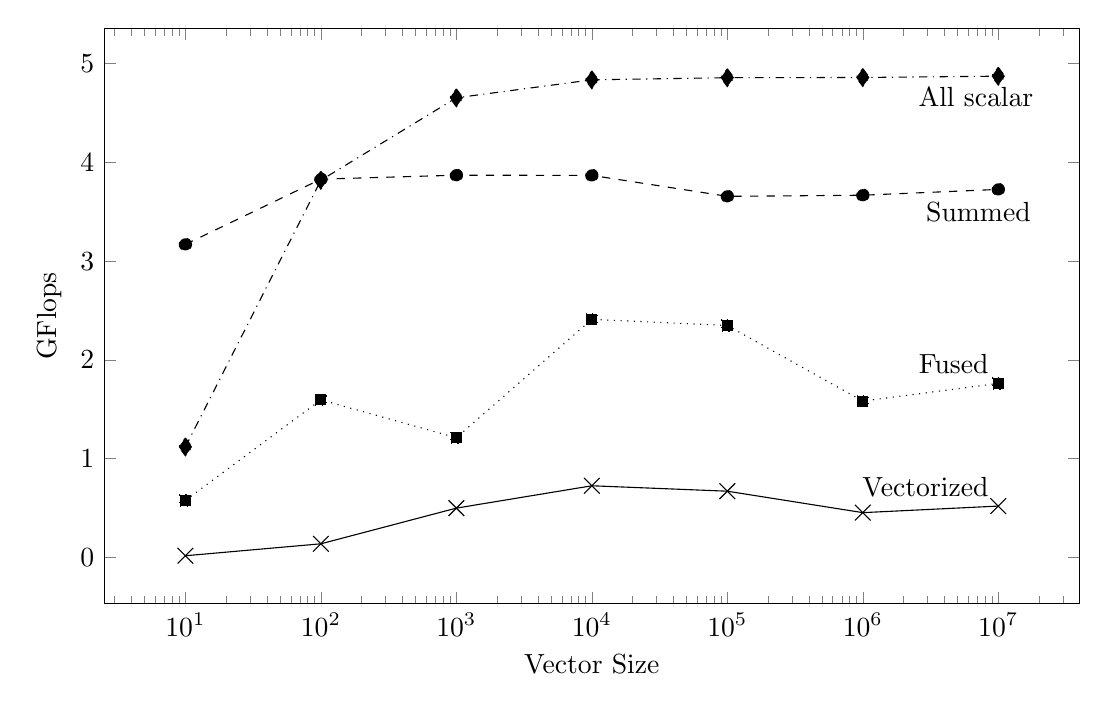
\begin{tikzpicture}
\begin{semilogxaxis}[
    %title=Vectorization Performance,
    xlabel={Vector Size},
    ylabel={GFlops},
    %legend entries={Vectorized, Fused, Summed, All scalar},
    %legend style={
    %  %at={(0.98,0.84)},
    %  legend pos = outer north east,
    %  anchor = north west,
    %  reverse legend=true
    %},
]
\addplot+[color=black,mark=x,mark options={scale=2,fill=black}] coordinates {
(10, 0.0181)
(100, 0.1390)
(1000, 0.5001)
(10000, 0.7263)
(100000, 0.6714)
(1000000, 0.4543)
(10000000, 0.5208)

}
node [pos=1,above left] {Vectorized};
\addplot+[color=black,mark=square*,mark options={fill=black},style=dotted] coordinates {
(10, 0.5778)
(100, 1.5960)
(1000, 1.2126)
(10000, 2.4110)
(100000, 2.3484)
(1000000, 1.5835)
(10000000, 1.7621)

}
node [pos=1,above left] {Fused};
\addplot+[color=black,style=dashed,mark=*,mark options={scale=1.1,fill=black}] coordinates {
(10, 3.1693)
(100, 3.8297)
(1000, 3.8697)
(10000, 3.8677)
(100000, 3.6557)
(1000000, 3.6670)
(10000000, 3.7258)

}
node [pos=0.9,below right] {Summed};
\addplot+[color=black,mark=diamond*,mark options={scale=1.6,fill=black},style=dashdotted] coordinates {
(10, 1.1202)
(100, 3.8186)
(1000, 4.6531)
(10000, 4.8348)
(100000, 4.8566)
(1000000, 4.8585)
(10000000, 4.8718)

}
node [pos=0.9,below right] {All scalar};
\end{semilogxaxis}
\end{tikzpicture}
\caption[Performance of vectorized code]{
\small{
  Performance of evaluating $x^2+x-1$ over a double precision vector of length $n$.
  Operation repeated $10^7/n$ times. (Core i7-3517U 1.9GHz, 4MB cache, 8GB RAM)
}
}
\label{fig:vecperf}
\end{figure}

However, this level of performance is not impressive compared to the
dashed line, which describes the operation rate for computing the
same results but summing them instead of storing them.
Finally, the dash-dotted line uses no memory at all, instead computing
input data points from a linear range.
Of course a real use case might require data to be read from memory or stored,
so this comparison is unfair (though not entirely, since many numerical
environments have represented even simple objects like linear ranges using
dense vectors \cite{matlabman:linspace}).
Still the point should be clear: vectors are not necessarily a good abstraction
for high performance.
The observation that memory is a bottleneck is not new, but for our purposes
the important point is that languages that only support vectorized syntax
cannot express the code rearrangements and alternate algorithms that can be
necessary to get the best performance.
A good technical computing language needs a more general interface to
performance.

The performance model resulting from vectorized syntax can be difficult to
understand, since it is difficult for users to predict which optimizations
will be applied.
A good example was discussed on the \texttt{julia-users} mailing list \cite{jasonmerrill}.
Jason Merrill discovered a Mathematica \cite{mathematica} list discussion
of the fastest way to count how many values fall within a given range.
Of many proposed implementations, the fastest turned out to be

\vspace{-3ex}

\[ \texttt{Total@Unitize@Clip[data,\{min,max\},\{0,0\}]} \]

\noindent
Arguably, it is difficult to know that this will run faster than, for
example,

\vspace{-3ex}

\[ \texttt{Count[data,~x\_/;~min<=x<=max]} \]

%% \begin{singlespace}
%% \begin{lstlisting}[language=julia]
%% function count_range(data, min, max)
%%     count = 0
%%     for elt in data
%%         if min < elt < max count += 1 end
%%     end
%%     count
%% end
%% \end{lstlisting}
%% \end{singlespace}

\iffalse
\subsection{What needs to be built in?}

It is often said that part of the usefulness of technical computing
environments comes from having many functions, and important abstractions
like matrices, ``built in''.

Built-in-ness often conflates two aspects:

\begin{enumerate}
\item A feature being readily available and agreed-on by all language users
\item A feature tightly coupled to the rest of the system
\end{enumerate}

(2) implies (1), but not the other way around. (2) is the only technically
interesting item, since the other can be addressed e.g.\  just by including
a library in the standard software distribution. Many technical computing
languages have done a large amount of (2) while justifying it with point (1).

While a large part of our motivation is to move more decisions and functionality
into libraries, it is equally important to identify what {\it must} be part of a
language for the system to be successful. We believe that large amounts of
functionality can be provided by add-ons, but that certain key features
cannot be. Past failures to properly classify features this way have
caused a lot of undue pain.

First, performance cannot be an add-on. If some users have a fast version of
a language and others have a slow version (with the difference being an
order of magnitude or more), library writers cannot be sure whether users
will find their code fast enough to be useful. How are we to teach people to
program in the language?

Psychologically, it may be difficult to accept a ``non standard'' extension
that changes a language so fundamentally. There is a nagging, though perhaps
totally unfounded, perception that something subtle may break. If indeed a
bug arises due to the use of such an extension, a user is likely to conclude
that the extension is dangerous or broken and stop using it. If, on the other
hand, a bug arises due to a language's standard optimizing compiler, the user
will simply file a bug report, then find a way to work around the problem.

Adding a JIT compiler to a language also requires acceptance of detriments
like compilation pauses and pages with RWX permissions. In some cases this
may lead to use of the extension being disallowed, perhaps for security
reasons.

Type systems similarly fail when provided as optional extensions. Library
writers face the same kinds of problems as with performance add-ons. Should I
use type annotations in my library?

Dynamic dispatch mechanisms also make especially poor add-ons. Of course,
every program makes decisions at run time, and so implements its own
``dispatch'' to some extent. But these behaviors are inextensible; if
language users do not agree on a reusable dispatch framework their code
will not be composable.
\fi

\subsection{Data representation}

There are two broad categories of programming language data models.
The first, favored by static languages, provides structures that are
complex and rigid but efficient.
Specific data types can be grouped and stored together with known
offsets and alignments.
Most data is stored directly, and pointer indirection must be
explicitly requested.
The second kind of data model, favored by dynamic languages,
prioritizes flexibility and simplicity.
Most data consists of pointers to tagged objects.
Indirection is the default.

It's reasonable to guess that these models would trade off about equally.
If you want the flexibility to substitute any kind of value in
any location at run time, making everything a pointer is the best
you can do.
The data layouts used by static languages require some
amount of metadata to describe, and manipulating this metadata
at run time could have significant overhead.
In the ``dynamic'' data model, even though everything is a pointer,
at least the code \emph{knows} that everything is a pointer, and so
does not waste time switching between different representations.

Interestingly, this intuition turns out not to be accurate.
As memory performance becomes a larger bottleneck, using less
space and avoiding indirection becomes more important.
Furthermore, most data in dynamic language programs is not as
dynamic as its authors might think, with homogeneous arrays
being quite common.
Good evidence for this claim was documented as part of work on
\emph{storage strategies}~\cite{Bolz2013}, a technique for
adapting dynamic languages to use more efficient representations.
The authors found that it was worthwhile to represent an array
as a wrapper providing a heterogeneous array interface on top of
a homogeneous array of varying type, even at the expense of
extra dispatch and occasionally changing the representation.

% ``storage strategies'' is simultaneously a great idea, and also a crack
% in the armor of typical dynamic languages big enough to tear them apart.

In some sense, our work takes this idea to its logical conclusion:
why not support a range of data representations from the beginning,
managed by a single sufficiently powerful dispatch system?
% so you need some type system, might as well be a good one


\section{A compiler for every problem}

In several prominent cases the language of a scientific sub-discipline is
so far removed from conventional programming languages, and the need for
performance is so great, that practitioners decide to write their own
compilers.
For example, the Tensor Contraction Engine~\cite{baumgartner2005synthesis}
accepts a mathematical input syntax describing tensor operations
used for electronic structure calculations in quantum chemistry.
The software performs many custom optimizations and finally generates
efficient parallel Fortran code.
Other examples of such scientific code generators include
Firedrake~\cite{Rathgeber2015} and FEniCS~\cite{LoggOlgaardEtAl2012a}
for FEM problems, PyOP2~\cite{pyop2} for general computations on meshes,
FFTW~\cite{FFTW05} for signal processing, and Pochoir~\cite{tang2011pochoir}
for stencil computations.

%\begin{itemize}
%\item The Tensor Contraction Engine~\cite{baumgartner2005synthesis}
%\item Firedrake~\cite{Rathgeber2015}, PyOP2 (vs. c++ libmesh)
%\item JuMP vs. python puLP and pyomo
%  (want to be able to pass functions, not C++ code as strings)
%  \ref{sec:jump}
%\item FFTW~\cite{FFTW05}
%\item pochoir~\cite{tang2011pochoir}
%\end{itemize}

%\cite{hopepython}

These systems can be highly effective, offering performance and productivity for
their problem domains that are not matched elsewhere.
In the long term, however, a proliferation of such projects would not be
a good thing.
It is substantially harder to reuse code between languages and compilers than
to reuse library code within a language, and it is harder to develop
a compiler than a library.
Mainstream languages have not been doing enough to facilitate these use
cases.
It would not be realistic to expect to replace all of these systems at once,
but Julia's style of type-based dispatch helps.
This will be discussed further in section~\ref{sec:stagedprogramming}.

%domain-specific languages
%``I've yet to hear anyone explain how you decide what are the boundaries of a 'domain-specific' language. Isn't the 'domain' mathematics and science itself?''
%https://existentialtype.wordpress.com/2013/07/22/there-is-such-a-thing-as-a-declarative-language/


\section{Social phenomena}

In the open source world, the architecture of a system can have social
implications.
Maintaining code in multiple languages, plus interface glue between them,
raises barriers to contribution.
Making the high-level language fast helps tremendously here, but there
are also cultural differences between programmers who understand
machine details and want more control, and those who are happy to use
defaults chosen by somebody else.
We will argue that it is possible to
%``easy polymorphism''
blend these styles, creating an effective compromise
between the two camps.
Evan Miller expressed this well as ``getting disparate groups of
programmers to code in the same language...With Julia, it's the domain experts
and the speed freaks.'' \cite{evanmiller}

This cultural difference often appears in the
form of a decision about what to express at the type level.
For example, imagine a user has linear algebra code that decides whether
to use the QR factorization or the LU factorization to solve a system:

\begin{singlespace}
\begin{lstlisting}[language=julia]
if condition
    M = qr(A)
else
    M = lu(A)
end
solve(M, x)
\end{lstlisting}
\end{singlespace}

\noindent
Initially, \texttt{qr} and \texttt{lu} might both return pairs of matrices.
Later, linear algebra library developers might decide that each function
should return a specialized type to store its factorization in a more
efficient format, and to provide dispatch to more efficient algorithms.
This decision should not break the user's intuition that the objects are
interchangeable in certain contexts.
We will discuss more extensive examples of such situations in
chapter~\ref{chap:casestudies}.

%% decisions about what to reflect at the type level should be less consequential
%% somebody might write a c++ library seeking max performance and so
%% might make array rank a static value.
%% (we will discuss this further in section~\ref{sec:ndindexing})
%% somebody else who wants dynamic flexibility might have to write an entirely
%% separate package.

%% Programming languages are observed to have strong network effects, and the
%% difficulty of getting new languages adopted is well known.
%% However based on \cite{meyerovich2012socio} we believe this doesn't have to
%% be the case.
%% The formula of improving or redesigning general-purposes languages to be more
%% appealing to domain experts might solve the problem.
%% That way the new system has immediate appeal for at least some users, without
%% the worry that a different tool will be needed as soon as requirements change
%% slightly.

\chapter{Design space}

% ``technology transfer'' from PLT to TC

This chapter will attempt to locate technical computing within the large
design space of programming languages.
It will discuss how the priorities introduced in section~\ref{sec:tcproblem}
relate to type systems and dispatch systems.
% concludes with an intro to julia etc.
Our lofty goal is to preserve the flexibility and ease of popular high level
languages, while adding the expressiveness needed for performant generic
programming.

% it is important to bear in mind the many meanings of the word ``type''
% often people use it just when they want a different ``kind of thing'',
% and have not yet thought about how that relates to the means of
% expression available.

\section{A binding time dilemma}
\label{sec:bindingtimedilemma}

Consider the following fragment of a function called \texttt{factorize},
which numerically analyzes a matrix to discover structure that
can be exploited to solve problems efficiently:

\begin{singlespace}
\begin{lstlisting}[language=julia]
if istril(A)
    istriu(A) && return Diagonal(A)
    utri1 = true
    for j = 1:n-1, i = j+1:m
        if utri1 && A[i,j] != 0
            utri1 = i == j + 1
        end
    end
    utri1 && return Bidiagonal(diag(A), diag(A, -1), false)
    return LowerTriangular(A)
end
\end{lstlisting}
\end{singlespace}

\noindent
The code returns different structured matrix types based on the input
data.
% TODO a bit more about how it's used
This sort of pattern can be implemented in object-oriented languages
by defining an interface or base class (perhaps called \texttt{StructuredMatrix}),
and declaring \texttt{Diagonal}, \texttt{Bidiagonal}, and so on as
subclasses.

Unfortunately, there are several problems with this solution.
Class-based OO ties together variation and dynamic dispatch: to allow
a value's representation to vary, each use of it needs to perform an
indirect call.
A major reason to use structured matrix types like \texttt{Bidiagonal}
is performance, so we'd rather avoid the overhead of indirect calls.
%for operations like element access.
A second problem is that most code operating on \texttt{Bidiagonal} would
be implementing algorithms that exploit its representation.
These algorithms would have to be implemented as methods of
\texttt{Bidiagonal}.
However this is not natural, since one cannot expect to have every
function that might be applied to bidiagonal matrices defined in
one place.
This kind of computing is function-oriented.
% other examples: CSC vs. CSR

Let's try a different abstraction mechanism: templates and overloading.
That would allow us to write code like this:

\begin{singlespace}
\begin{lstlisting}[language=julia]
if diagonal
    solve(Diagonal(M), x)
elseif bidiagonal
    solve(Bidiagonal(M), x)
end
\end{lstlisting}
\end{singlespace}

\noindent
Here, structured matrix types are used to immediately select an
implementation of \texttt{solve}.
But the part that selects a matrix type can't be abstracted away.
We would like to be able to write \texttt{solve(factorize(M), x)}.

% TODO: or tagged unions, but then you have to handle every case

%... no wonder people use prepackaged version of this functionality
Given these constraints, the traditional design of technical
computing systems makes sense: pre-generate a large number of
optimized routines for various cases, and be able to dispatch
to them at run time.

It's clear what's going on here: mathematics is dependently typed.
If a compiler could prove that a certain matrix were bidiagonal, or
symmetric, there would be no problem.
But knowing what a given object \emph{is} in a relevant sense can
require arbitrary proofs, and in research computing these proofs
might refer to objects that are not yet well understood.
% In numerical computing, if \emph{anybody} were able to prove the
% relevant property, there would be no point in running the program.

Most languages offer a strict divide between early and late binding,
separated by what the type system can statically prove.
The less the type system models the domain of interest, the more it
gets in the way.
% talk about the premature optimization of assuming
% (generate code for) = (known at compile time)
The compiler's ability to generate specialized code is also coupled
to the static type system, preventing it from being reused for domains
the type system does not handle well.
In general, of course, lifting this restriction implies a need to
generate code at run time, which is not always acceptable.
However run time code generation might not be necessary in every case.
A compiler could, for example, automatically generate a range of
specialized routines and select among them at run time, falling back
to slower generic code if necessary.

Consider the trade-off this entails.
The programmer is liberated from worrying about the binding time of
different language constructs.
With a JIT compiler, performance will probably be good.
But without JIT, performance will be unpredictable, with no clear
syntactic rules for what is expected to be fast.
So it is not surprising that software engineering languages shun this
trade-off.
However we believe it is the trade-off technical computing
users want by default, and it has not generally been available
in any language.

Designing for this trade-off requires a change of perspective
within the compiler.
Most compilers focus on, and make decisions according to, the
language's source-level type system.
Secondarily, they will perform flow analysis to discover
properties not captured by the type system.
Given our goals, we need to invert this relationship.
The focus needs to be on understanding program behavior
\emph{as thoroughly as possible}, since no one set of rules
will cover all cases.
Usually changing a language's type system is a momentous event,
but in the analysis-focused perspective the compiler can evolve
rapidly, with ``as thoroughly as possible'' handling more cases
all the time.
This approach is still compatible with static typing, although we will not
discuss it much.
We could pick a well-defined subset of the system,
or a separate type system, to give errors about.

The notion of ``as thorough as possible'' analysis is formalized
by domain theory.

%Instead of a split between static and dynamic resolution, we can
%instead focus on program \emph{analysis}.
%The goal is to understand a program as well as possible.

%2 problems?
%   1 - flexibility implies late binding, slowness. e.g. CSR/CSC as classes
%   2 - given a simple type system, programs will not match the lattice
%       and analysis diverges

% issues:
% - how programs make choices
% - how compiler-understandable are those choices
% - when do you get specialized code

\section{Domain theory}

In the late 1960s Dana Scott and Christopher Strachey asked how to assign
meanings to programs, which otherwise just appear to be lists of symbols
\cite{scott1971toward}.
For example, given a program computing the factorial function, we
want a process by which we can assign the meaning ``factorial'' to it.
This led to the invention of domain theory, which can be interpreted
as modeling the behavior of a program without running it.
A ``domain'' is essentially a partial order of sets of values that a
program might manipulate.
The model works as follows: a program starts with no
information, the lowest point in the partial order (``bottom'').
Computation steps accumulate information, gradually moving higher through
the order.
This model provides a way to think about the meaning of a program without
running the program.
Even the ``result'' of a non-terminating program has a representation
(the bottom element).
%Other elements of the partial order might refer to intermediate results.

The idea of ``running a program without running it'' is of great interest
in compiler implementation.
A compiler would like to discover as much information as possible about a
program without running it, since running it might take a long time, or
produce side effects that the programmer does not want yet, or, of course,
not terminate.
The general recipe for doing this is to design a partial order (lattice)
that captures program properties of interest, and then describe all
primitive operations in the language based on how they transform
elements of this lattice.
Then an input program can be executed, in an approximate sense, until
it converges to a fixed point.
%For example, given a program that outputs an integer, we might decide
%that we only care whether this integer is even or odd.
%Then our posets are the even and odd integers, and we will classify operations
%in the program according to whether they are evenness-preserving,
%evenness-inverting, always even, always odd, of uncertain evenness,
%etc.
Most modern compilers use a technique like this
(sometimes called abstract interpretation \cite{abstractinterp})
to semi-decide
interesting properties like whether a variable is a constant, whether
a variable might be used before it is initialized, whether a variable's
value is never used, and so on.
%Domain theory gave rise to the study of denotational semantics and the
%design of type systems. However, the original theory is quite general
%and invites us to invent any domains we wish for any sort of language.
%Abstract interpretation \cite{abstractinterp} is an especially
%elegant and general implementation of this idea.
%It should be clear that this sort of analysis, while clearly related
%to type systems, is fairly different from what most programmers
%think of as type \emph{checking}.

Given the general undecidability of questions about programs, analyses
like these are \emph{conservative}.
If our goal is to warn programmers about use of uninitialized
variables, we want to be ``better safe than sorry'' and print a warning
if such a use \emph{might} occur.
Such a use corresponds to any lattice element greater than or equal to
the element representing ``uninitialized''.
Such conservative analyses are the essence of compiler transformations
for performance (optimizations): we only want to perform an optimization
if the program property it relies on holds for sure.
% and not if there is any uncertainty.

The generality of this approach
allows us to discover a large variety of program properties as long as we are
willing to accept some uncertainty.
%Of course, many programmers and language designers prefer to maximize
%safety, leading to different approaches that trade away some precision
%(e.g. syntactic type systems such as those in the ML language
%family \cite{hindley1969principal, MLtypeinf}).
Even if static guarantees are not the priority, or if a language considers
itself unconcerned with ``types'', the domain-theoretic model is
still our type system in some sense, whether we like it or not
(as implied by \cite{scott1976data}).

%- make it easier to ``follow the lattice''
% analyses don't work as well with programs not written to be
% ``type conscious''.
% the solution is just to make it easier to write type conscious programs.
% this doesn't require any restrictions, just a stylistic change.
% you would think if types are also just data values there would be no
% gain, but there is.
% there are run time things, and just flow-sensitive things

\subsection{Programs and domains}
\label{sec:programsanddomains}

% - checking isbidiag() vs. having a type
% - checking every array elt for integer - maybe for ^ function

Program analyses of this kind have been applied to high-level
languages many times.
A common pitfall is that the analysis can easily \emph{diverge}
for programs that make distinctions not modeled by the lattice.

Consider the following program that repeatedly applies elementwise
exponentiation (\texttt{.\^}) to an array:

% TODO: what should `f` be?
% maybe A = [sum(A.^A)]
\begin{singlespace}
\begin{lstlisting}[language=julia]
A = [n]
for i = 1:niter
    A = f(A .^ A)
end
return A
\end{lstlisting}
\end{singlespace}

\noindent
We will try to analyze this program using the lattice in figure~\ref{fig:arraylattice}.

% TODO maybe add Union(Array{Int},Array{BigInt}) to this
\begin{figure}[!t]
\begin{center}
\begin{tikzpicture}[node distance=2cm]
\node(top)   {$\top$};
\node(Array)         [below=0.5cm of top] {\texttt{Array}};
\node(ArrayInteger)  [below=0.5cm of Array] {$\exists\ T<:\texttt{Integer}\ \texttt{Array\{T\}}$};
\node(ArrayInt)      [below left=1cm of ArrayInteger] {\texttt{Array\{Int\}}};
\node(ArrayBigInt)   [below right=1cm of ArrayInteger] {\texttt{Array\{BigInt\}}};
\node(ArrayFloat)    [right=1.25cm of ArrayBigInt] {\texttt{Array\{Float\}}};
\node(bot)   [below=4.5cm of top] {$\bot$};
\draw(top) -- (Array);
\draw(Array) -- (ArrayInteger);
\draw(ArrayInteger) -- (ArrayInt);
\draw(ArrayInteger) -- (ArrayBigInt);
\draw(Array) -- (ArrayFloat);
\draw(ArrayInt) -- (bot);
\draw(ArrayBigInt) -- (bot);
\draw(ArrayFloat) -- (bot);
\end{tikzpicture}
\end{center}
\caption{
  A lattice of array types
}
\label{fig:arraylattice}
\end{figure}

The result depends strongly on how the \texttt{.\^} and \texttt{\^} functions
are defined (assume that \texttt{.\^} calls \texttt{\^} on every element of an array).
The code might look like this:

\vspace{-4ex}
\begin{singlespace}
\begin{multicols}{2}
\begin{lstlisting}[language=julia]
function ^(x, y)
    if trunc(y) == y
        if overflows(x, y)
            x = widen(x)
        end
        # use repeated squaring
    else
        # floating point algorithm
    end
end


function f(a)
    if all(trunc(y) .== y)
        # integer case
    else
        # general case
    end
end
\end{lstlisting}
\end{multicols}
\end{singlespace}

\noindent
This code implements the user-friendly behavior of automatically switching to the
\texttt{BigInt} type on overflow, by calling \texttt{widen}.

Assume we initially know that \texttt{n} is an \texttt{Int}, and therefore
that \texttt{A} is an \texttt{Array\{Int\}}.
Although \texttt{A} really does have this type, the code does not mention
types anywhere.
Next, the type of an element taken from \texttt{A} (\texttt{Int}) will
flow to the \texttt{y} argument of \texttt{\^}.
The function's behavior crucially depends on the test \texttt{trunc(y) == y}.
It is always true for integer arguments, but it is unlikely that the
analysis can determine this.
Therefore \texttt{\^} might return an \texttt{Int}, \texttt{BigInt}, or
\texttt{Float}, and we can only conclude that \texttt{A.\^{}A} is an
\texttt{Array}.
When function \texttt{f} is called, it performs a fairly expensive test
to see if every element is an integer.
Only through human reasoning about the whole program do we see that
this test is unnecessary.
However when the analysis considers \texttt{f} applied to type
\texttt{Array}, our type information is likely to diverge further to
\texttt{$\top$}, since we don't know anything about the array's elements.

The problem is that the program is not written in terms of the
underlying value domain, even though it could be.
We might have written \texttt{isa(y,Integer)} instead of \texttt{trunc(y) == y}.
However, there are reasons that code like this might exist.
The programmer might not be aware of the type system, or the conditional
might refer to a property that was not originally reflected in the type system
but is later, as the language and libraries evolve.
Adding type declarations is not an ideal solution since it can restrict
polymorphism, and the programmer might not know the type of \texttt{A.\^{}A}
or even the type of \texttt{n}.


\iffalse
How can we fix this?
One solution is to add type annotations.
But the author of the original code does not know the type of
\texttt{A.\^{}A}, and might not even know the type of \texttt{n}.
%%%%%  is this accurate?
Another solution is to improve the analysis.
But we will never finish adding cases to the compiler.
Perhaps we can handle \texttt{trunc(y) == y}, but will we also be
able to understand \texttt{trunc(y) == 1*y}?
\fi

Our solution is to give some simple tools to the library developer
(who, of course, is not necessarily a different person).
In Julia, one can implement \texttt{\^} and \texttt{f} as follows:

\begin{singlespace}
\begin{lstlisting}[language=julia]
function ^(x, y)
    # original code
end

function ^(x, y::Integer)
    if overflows(x, y)
        x = widen(x)
    end
    # ...
end

function f(a)
    # original code
end

function f{T<:Integer}(a::Array{T})
    # integer case
end
\end{lstlisting}
\end{singlespace}

\noindent
The syntax \texttt{y::Integer} for a function argument is a dispatch specification.
Now, from the same source program, we can conclude that only
\texttt{\^{}(x, y::Integer)} is applicable, so we know that the
result of \texttt{A.\^{}A} is some integer array.
The library writer can intercept this case with the definition
\texttt{f\{T<:Integer\}(a::Array\{T\})}\footnote{
Although the signature of this method happens to match one of the
lattice elements in figure~\ref{fig:arraylattice}, this is a coincidence.
Method applicability is determined dynamically.
}, avoiding the check \texttt{all(trunc(y) .== y)}.
Since we started with an integer array, the whole program behaves
exactly as before.

We have neither added restrictions, nor asked for redundant type annotations.
All we did is add a dispatch system, and encourage people to use it.
Using dispatch in this way is optional, but comes with benefits for
structuring programs.
For example, the function \texttt{f} above might perform much better
on integer arrays.
We can implement this case separately from the checks and extra logic
that might be needed for other data types, leading to cleaner code
and also making the core definition of \texttt{f} smaller and therefore
more likely to be inlined.

% TODO something about why we use an extensibility mechanism for collecting
% type info.
% 1 - the extra cases can be added by somebody else
% 2 - a library can pick a type to return to user code, and later
%     ``intercept'' operations on it

The original version of this code can also be written in our system,
though it probably will not perform as well.
However, it might still perform better than one would expect, since the
functions that it calls are in turn defined using the same dispatch
mechanism.
This mechanism is expressive enough to be used down to the lowest levels of
the system, providing leverage one would not get from an object system
or performance add-on.

% reverse flow
Having type information attached to user or library definitions
increases the value of \emph{reverse} data flow analysis.
One way to describe why analyses of highly dynamic code diverge
is that everything in the program monotonically increases the
number of cases we need to consider; there is no way to
narrow possibilities.
But if we know that a function is only defined on type \texttt{T},
every value that passes through its argument list is narrowed to
\texttt{T}.

% there seems to be some psychology to this: ``write method definitions''
% is somehow an easier performance model than ``use conditions only involving
% type checks''
% instead of requiring that the compiler be able to resolve things, we
% just want to make it more likely.

% isa(x,Int) is simple enough, but for more complicated checks it becomes
% much harder to predict. e.g. imagine testing for everything being the
% same type.
% there has to be a split between what is specialized on and what is not.
% in c++ this requires switching to templates.


% next we will consider how this dispatch system fits in

\section{Dispatch systems}

It would be unpleasant if every piece of every program we wrote were forced
to do only one specific task.
Every time we wanted to do something slightly different, we'd have to write
a different program.
But if a language allows the same program element to do different things at
different times, we can write whole classes of programs at once.
This kind of capability is one of the main reasons object-oriented programming
is popular: it provides a way to automatically select different behaviors
according to some structured criteria
(we use the non-standard term ``criteria'' deliberately, in order
to clarify our point of view, which is independent of any particular
object system).

However in class-based OO there is essentially \emph{no way} to create an
operation that dispatches on existing types.
This has been called ``the expression problem''~\cite{wadler1998expression}).
While many kinds of object-oriented programs can ignore or work around
this problem, technical programs cannot.
In this domain most programs deal with the same
few types (e.g.\ numbers and arrays), and might sensibly want to write new
operations that dispatch on them.

% The loss of encapsulation due to multimethods weighed in \cite{binarymethods}
% is less of a problem for technical computing, and in some cases even
% advantageous.

%Somewhat unfortunately, the term \emph{object-oriented} has many
%connotations, and the \emph{object-oriented} methodology tries to address
%multiple software engineering problems --- for example modularity,
%encapsulation, implementation hiding, and code reuse. These issues are
%important, but it may be because of them that over time too little
%emphasis has been placed on expressive power.

\subsection{A hierarchy of dispatch}

%The sophistication of the available ``selection criteria'' account for a
%large part of the perceived ``power'' or leverage provided by a language.
It is possible to illustrate a hierarchy of such mechanisms.
As an example, consider a simple simulation, and how it can be written
under a series of increasingly powerful paradigms. First, written-out
imperative code:

\vspace{-3ex}
\begin{singlespace}
\begin{verbatim}
while running
    for a in animals
        b = nearby_animal(a)
        if a isa Rabbit
            if b isa Wolf then run(a)
            if b isa Rabbit then mate(a,b)
        else if a isa Wolf
            if b isa Rabbit then eat(a,b)
            if b isa Wolf then follow(a,b)
        end
    end
end
\end{verbatim}
\end{singlespace}

We can see how this would get tedious as we add more kinds of animals
and more behaviors.
Another problem is that the animal behavior is
implemented directly inside the control loop, so it is hard to see
what parts are simulation control logic and what parts are animal
behavior.
Adding a simple object system leads to a nicer implementation
\footnote{A perennial problem with simple examples is that better
implementations often make the code longer.}:

\vspace{-3ex}
\begin{singlespace}
\begin{verbatim}
class Rabbit
    method encounter(b)
        if b isa Wolf then run()
        if b isa Rabbit then mate(b)
    end
end

class Wolf
    method encounter(b)
        if b isa Rabbit then eat(b)
        if b isa Wolf then follow(b)
    end
end

while running
    for a in animals
        b = nearby_animal(a)
        a.encounter(b)
    end
end
\end{verbatim}
\end{singlespace}

Here all of the simulation's animal behavior has been
compressed into a single program point: \texttt{a.encounter(b)}
leads to all of the behavior by selecting an implementation based
on the first argument, \texttt{a}.
This kind of criterion is essentially indexed lookup; we can imagine
that \texttt{a} could be an integer index into a table of operations.

The next enhancement to ``selection criteria'' adds a hierarchy
of behaviors, to provide further opportunities to avoid repetition.
Here \texttt{A<:B} is used to declare a subclass relationship; it
says that an \texttt{A} is a kind of \texttt{B}:

\vspace{-3ex}
\begin{singlespace}
\begin{multicols}{2}
\begin{verbatim}
abstract class Animal
    method nearby()
        # search within some radius
    end
end

class Rabbit <: Animal
    method encounter(b::Animal)
        if b isa Wolf then run()
        if b isa Rabbit then mate(b)
    end
end

class Wolf <: Animal
    method encounter(b::Animal)
        if b isa Rabbit then eat(b)
        if b isa Wolf then follow(b)
    end
end

while running
    for a in animals
        b = a.nearby()
        a.encounter(b)
    end
end
\end{verbatim}
\end{multicols}
\end{singlespace}

We are still essentially doing table lookup, but the tables have
more structure: every \texttt{Animal} has the \texttt{nearby}
method, and can inherit a general purpose implementation.

This brings us roughly to the level of most popular object-oriented
languages.
But still more can be done.
Notice that in the first transformation we replaced one level of \texttt{if}
statements with method lookup.
However, inside of these methods a structured set of \texttt{if} statements
remains.
We can replace these by adding another level of dispatch.

\vspace{-3ex}
\begin{singlespace}
\begin{verbatim}
class Rabbit <: Animal
    method encounter(b::Wolf) = run()
    method encounter(b::Rabbit) = mate(b)
end

class Wolf <: Animal
    method encounter(b::Rabbit) = eat(b)
    method encounter(b::Wolf) = follow(b)
end
\end{verbatim}
\end{singlespace}

We now have a \emph{double dispatch} system, where a method call
uses two lookups, first on the first argument and then on the
second argument.
This syntax might be considered a bit nicer, but the design
begs a question: why is $n=2$ special?
It isn't, and we could consider even more method arguments as part of
dispatch.
But at that point, why is the first argument special?
Why separate methods in a special way based on the first argument?
It seems arbitrary, and indeed we can remove the special treatment:

\vspace{-3ex}
\begin{singlespace}
\begin{verbatim}
abstract class Animal
end

class Rabbit <: Animal
end

class Wolf <: Animal
end

nearby(a::Animal)               = # search
encounter(a::Rabbit, b::Wolf)   = run(a)
encounter(a::Rabbit, b::Rabbit) = mate(a,b)
encounter(a::Wolf, b::Rabbit)   = eat(a, b)
encounter(a::Wolf, b::Wolf)     = follow(a, b)

while running
    for a in animals
        b = nearby(a)
        encounter(a, b)
    end
end
\end{verbatim}
\end{singlespace}

Here we made two major changes: the methods have been moved ``outside''
of any classes, and all arguments are listed explicitly.
This is sometimes called \emph{external dispatch}.
This change has significant implications.
Since methods no longer need to be ``inside'' classes, there is no syntactic
limit to where definitions may appear.
Now it is easier to add new methods after a class has been defined.
Methods also now naturally operate on combinations of objects, not single objects.
%There may be software engineering reasons to want ``ownership'' of methods
%by objects, but strictly speaking this coupling does not seem correct.
%It ought to be possible to define function behaviors independently of
%data hiding concerns.

The shift to thinking about combinations of objects is fairly revolutionary.
Many interesting properties only apply to combinations of objects, and not
individuals.
We are also now free to think of more exotic kinds of combinations.
We can define a method for \emph{any number} of objects:

\begin{verbatim}
encounter(ws::Wolf...) = pack(ws)
\end{verbatim}

\noindent
We can also abstract over more subtle properties, like whether the
arguments are two animals of the same type:

\begin{verbatim}
encounter{T<:Animal}(a::T, b::T) = mate(a, b)
\end{verbatim}

\noindent
Some systems push dispatch expressiveness even further.
% TODO more


\subsection{Predicate dispatch}

%Patterns are very powerful, but the tradeoff is that there is not
%necessarily a useful relationship between what your program does and
%what a static analysis (based on a finite-height partial order over
%patterns) can discover. Maybe julia could be considered a sweet spot
%somewhere in between.

Predicate dispatch is a powerful object-oriented mechanism that allows
methods to be selected based on arbitrary predicates \cite{ErnstKC98}.
It is, in some sense, the most powerful \emph{possible} dispatch system,
since any computation may be done as part of method selection.
Since a predicate denotes a set (the set of values for which it is true),
it also denotes a set-theoretic type.
Some type systems of this kind, notably that of Common
Lisp~\cite{steele1990common:types}, have actually included predicates as types.
However, such a type system is obviously undecidable, since it
requires computing the predicates themselves or, even worse, computing
predicate implication.\footnote{
Many type systems involving bounded quantification, such as system $F_{<:}$,
are already undecidable \cite{Pierce1994131}.
However, they seem to terminate for most practical programs, and also admit
minor variations that yield decidable systems \cite{Castagna:1994:DBQ:174675.177844}.
It is fair to say they are ``just barely'' undecidable, while predicates
are ``very'' undecidable.
}

For a language that is willing to do run time type checks anyway, the
undecidability of predicate dispatch is not a problem.
Interestingly, it can also pose no problem for \emph{static} type systems
that wish to prove that every call site has an applicable method.
Even without evaluating predicates, one can prove that the available methods
are exhaustive (e.g.\ methods for both $p$ and $\neg p$ exist).
In contrast, and most relevant to this thesis, predicate types \emph{are} a
problem for code \emph{specialization}.
Static method lookup would require evaluating the predicates, and optimal code
generation would require understanding something about what the predicates mean.
One approach would be to include a list of satisfied predicates in a type.
However, to the extent such a system is decidable, it is essentially equivalent
to multiple inheritance.
Another approach would be to separate predicates into a second ``level'' of the
type system.
The compiler would combine methods with the same ``first level'' type, and then
generate branches to evaluate the predicates.
Such a system would be useful, and could be
combined with a language like Julia or, indeed, most object-oriented
languages (this has been done for Java~\cite{Millstein:2009:EMP:1462166.1462168}).
However this comes at the expense of making predicates second-class
citizens of the type system.

In considering the problems of predicate dispatch for code specialization,
we seem to be up against a fundamental obstacle: some sets of values are
simply more robust under evaluation than others.
Programs that map integers to integers abound, but programs that map, say,
even integers to even integers are rare to the point of irrelevance.
With predicate dispatch, the first version of the code in
section~\ref{sec:programsanddomains} could have been rearranged to use
dispatch instead of \texttt{if} statements.
This might have advantages for readability and extensibility, but not for
performance.


\subsection{Symbolic programming}

Systems based on symbolic rewrite rules arguably occupy a further tier of
dispatch sophistication.
In these systems, you can dispatch on essentially anything, including arbitrary
values and structures.
Depending on details, their power is roughly equal to that of predicate
dispatch.
%These systems are typically powerful enough to concisely define the kinds of
%behaviors we are interested in.

However, symbolic programming lacks data abstraction: the concrete
representations of values are exposed to the dispatch system.
In such a system, there is no difference between being a list and being
something \emph{represented} as a list.
If the representation of a value changes, the value can be inadvertently
``captured'' by a dispatch rule that was not intended to apply to it,
violating abstraction.
% we use 2-part values instead; symbolic part and data part effectively

There has always been a divide between ``numeric'' and ``symbolic''
languages in the world of technical computing.
To many people the distinction is fundamental, and we should happily live
with both kinds of languages.
But if one insists on an answer as to which approach is the right one,
then the answer is: symbolic.
Programs are ultimately symbolic artifacts.
Computation is limited only by our ability to describe it, and
symbolic tools are needed to generate, manipulate, and query these
descriptions.
For example in numerical computing, a successful approach has been to
create high-performance kernels for important problems.
From there, the limiting factor is knowing \emph{when} to use each
kernel, which can depend on many factors from problem structure to
data size.
Symbolic approaches can be used to automate this.
We will see some examples of this in chapter~\ref{chap:casestudies}.

\subsection{Choices, choices}
\label{sec:choices}

\newcommand{\chk}{{\Large \checkmark}}

\begin{table}[!t]
\begin{center}
\begin{tabular}{|c||c|c|c|c|c|c|c|}
\hline
               & Domain &  Dynamic  & Spec. & Pattern & S.T.S. & S.C. \\
\hline
\hline
Methods        & $O(1)$   &         &       &         & \chk   & \chk \\
\hline
Virtual methods  & $O(1)$   & \chk    &       &         & \chk   & \chk \\
\hline
Overloading    & $O(n)$   &         &       &         & \chk   & \chk \\
\hline
Templates      & $O(n)$   &         & \chk  &         & \chk   &      \\
\hline
Closures       & $O(1)$   & \chk    &       &         & \chk   & \chk \\
\hline
Duck typing    & $O(1)$   & \chk    &       &         &        & \chk \\
\hline
Multimethods   & $O(n)$   & \chk    &       &         & ?      & ?    \\
\hline
Predicate dispatch & $O(n m)$ & \chk    &       &  \small{1}  & ? & ? \\
\hline
Typeclasses    & $O(m)$   & \small{2} & \small{3} &   & \chk   & \chk \\
\hline
Term rewriting & $O(n m)$ & \chk    &       & \chk    &        &      \\
\hline
Julia          & $O(n m)$ & \chk    & \chk  &         & ?      &      \\
\hline
\end{tabular}
\end{center}
\begin{singlespace}
\caption[Attributes of code selection features]{
\small{
Attributes of several code selection features.
Spec.\ stands for specialization.
S.T.S.\ stands for statically type safe.
S.C.\ stands for separate compilation.
1.\ Depending on design details, 2.\ When combined with existential types,
3.\ Optionally, with declarations,
% no, because it can only pattern match on types
%4.\ With the \texttt{FlexibleInstances} option.
}
}
\label{table:dispatch}
\end{singlespace}
\end{table}

% message of the table: you have to know a really large amount to
% pick which one of these to use. there is no best one.
% ``domain'' languages are all about avoiding knowledge of this table.

Table~\ref{table:dispatch} compares 11 language features.
Each provides some sort of control flow indirection, packaged into a
structure designed to facilitate reasoning (ideally human reasoning,
but often the compiler's reasoning is prioritized).
The ``domain'' column describes the amount of information considered
by the dispatch system, where $n$ is the number of arguments and
$m$ is the amount of relevant information per argument.
$O(1)$ means each use of the feature considers basically the same
amount of information.
$O(n)$ extends the process to every argument.
$O(m)$ means that one value is considered, but its structure is
taken into account.
Squares with question marks are either not fully understood, or too
sensitive to design details to answer definitively.

%% it may be that the ``power'' of a language is measured by the complexity
%% of the criteria used by the language's run time dispatch mechanisms.

This table illustrates how many combinations of dispatch semantics have
been tried.
Keeping track of these distinctions is a distraction when one is focused
on a non-programming problem.
Including more than one row of this table makes a language especially
complex and difficult to learn.

% compare to julia tradeoffs


\section{Subtyping}
\label{sec:chap3subtyping}

So far we have seen some reasons why dispatch contributes significantly
to flexibility and performance.
However we have only actually dispatched on fairly simple properties like
whether a value is an integer.
How powerful should dispatch be, exactly?
Each method signature describes some set of values to which it applies.
Some signatures might be more specific than others.
The theory governing such properties is subtyping.

% TODO
% informal convexity property. ``any # of integers'' is ok, but
% ``any # of integers except 3'' is not.
%% reflect on level of power: this dispatch system is both more and less
%% powerful than previous ones in various ways.

% normally this is used for type safety
% in our case it is used to form an ``analyzable subset'' of the language

It turns out that a lot of relevant work on this has been done in the
context of type systems for XML~\cite{hosoya2000xduce, BCF03}.
%Something about semantic subtyping and type systems for processing XML.
XML at first seems unrelated to numerical computing, and indeed it
was quite a while before we discovered these papers and noticed the
overlap.
However if one substitutes ``symbolic expression'' for ``XML document'',
the similarity becomes clearer.
In XML processing, programs match documents against patterns in order
to extract information of interest or validate document structure.
These patterns resemble regular expressions, and so also denote sets.
%and admit a subset (subtype) relation.

In our context, some argument lists and the properties of some data
structures are sufficiently complex to warrant such a treatment.
For example, consider a \texttt{SubArray} type that describes a
selection or ``view'' of part of another array.
Here is part of its definition in Julia's standard library:

\begin{singlespace}
\begin{lstlisting}[language=julia]
const ViewIndex = Union(Int, Colon, Range{Int}, UnitRange{Int},
                        Array{Int,1})
immutable SubArray{T, N, P<:AbstractArray,
                   I<:Tuple{ViewIndex...}} <: AbstractArray{T,N}
\end{lstlisting}
\end{singlespace}

\noindent
The properties of the \texttt{SubArray} type are declared within curly
braces.
A \texttt{SubArray} has an element type, number of dimensions,
underlying storage type, and a tuple of indexes (one index per dimension).
Limiting indexes to the types specified by \texttt{ViewIndex}
documents what kind of indexes can be supported efficiently.
Different index tuples can yield drastically different performance
characteristics.

Without the ability to describe these properties at the type level,
it would be difficult to implement an efficient \texttt{SubArray}.
In section~\ref{sec:programsanddomains} we only needed to test fairly
simple conditions, but the checks here would involve looping over
indexes to determine which dimensions to drop, or to determine whether
stride-1 algorithms can be used, and so on.
% TODO more

% our language is in many ways dual to ML. that family shuns subtyping,
% but in the lattice theoretic model it's inescapable.
%\cite{hindley1969principal, MLtypeinf}


\section{Specialization}

\subsection{Parametric vs.\ ad hoc polymorphism}

The term \emph{polymorphism} refers generally to reuse of code or data
structures in different contexts.
A further distinction is often made between \emph{parametric} polymorphism
and \emph{ad hoc} polymorphism.
Parametric polymorphism refers to code that is reusable for many types
because its behavior does not depend on argument types (for example,
the identity function).
%reusing the \emph{same} code for different purposes, while
Ad hoc polymorphism refers to selecting
\emph{different} code for different circumstances.

%% Both forms occur frequently in technical computing.
%% For example, a programmer intuitively expects that \texttt{A[i]} selects
%% an element of an array regardless of what kind of array \texttt{A} is.
%% \texttt{A} might contain integers or strings, it might be a local
%% array or a distributed array, and so on.
%% This is parametric polymorphism.
%% However the ``parametric'' property only applies to the code \texttt{A[i]}
%% itself.
%% When we dig into how array indexing actually works, we will probably
%% need to resort to ad hoc polymorphism.
%% For example, when \texttt{A} is a local array the code accesses local
%% memory, and when \texttt{A} is distributed it might be necessary to
%% send a network message instead.
%% At a lower level, the machine code for \texttt{A[i]} needs to be
%% different depending on the array's element type.

In theory, a parametrically polymorphic function works on all data
types.
In practice, this can be achieved by forcing a uniform representation of
data such as pointers, which can be handled by the same code regardless of
what kind of data is pointed to.
However this kind of representation is not the most efficient, and
for good performance specialized code for different types must be
generated.

The idea of specialization unites parametric and ad hoc polymorphism.
Beginning with a parametrically polymorphic function, one can imagine
a compiler specializing it for various cases, i.e.\ certain concrete argument
values or types.
These specializations could be stored in a lookup table, for use
either at compile time or at run time.

Next we can imagine that the compiler might not optimally specialize
certain definitions, and that the programmer would like to provide
hints or hand-written implementations to speed up special cases.
For example, imagine a function that traverses a generic array.
A compiler-generated specialization might inline a specific array type's
indexing operations, but a human might further realize that the loop order
should be switched for certain arrays types based on their storage order.

However, if we are going to let a human specialize a function for performance,
we might as well allow them to specialize it for some other reason, including
entirely different behavior.
But at this point separate ad hoc polymorphism is no longer necessary; we are
using a single overloading feature for everything.

\iffalse
Parametric polymorphism describes code that works for any object precisely
because it does not do anything meaningful to the object, for example the
identity function. In contrast, programming with tagged data (e.g.
symbolic expression systems, XML) permits code to work for any object
because every object has the same structure, allowing meaningful
operations.
\fi

\subsection{Separate compilation}

Writing the signature of a generic method that needs to be separately compiled,
as in Java, can be a difficult exercise.
The programmer must use the type system to write down sufficient conditions on all
arguments.
The following example from a generic Java graph
library~\cite{Garcia:2003:CSL:949305.949317} demonstrates the level of verbosity
that can be required:

\begin{singlespace}
\begin{lstlisting}[language=java,style=ttcode]
public class breadth_first_search {
  public static<Vertex, Edge extends GraphEdge<Vertex>,
                VertexIterator extends Iterator<Vertex>,
                OutEdgeIterator extends Iterator<Edge>,
                Visitor extends BFSVisitor,
                ColorMap extends ReadWriteMap<Vertex, Integer>>
  void go(VertexListAndIncidenceGraph<Vertex,Edge,
            VertexIterator,VerticesSizeType,OutEdgeIterator,
            DegreeSizeType> g,
          Vertex s, ColorMap c, Visitor vis);
}
\end{lstlisting}
\end{singlespace}

%(other problems: primitive types int and double cannot be used,
%static parameters can only be inferred directly from arguments,
%not from constraints of other parameters. our subtyping system
%does not have this problem)

If, however, we are going to specialize the method, the compiler can analyze it
using actual types from call sites, and see for itself whether the method works
in each case.
This is how C++ templates are type checked; they are analyzed again for each
instantiation.

It is quite interesting that performance and ease-of-use pull this design
decision in the same direction.


\section{Easy polymorphism}

% conclude by summarizing the design decisions we end up with:

% easy polymorphism recipe:

The total effect of these design considerations is something more than the
sum of the parts.
We obtain what might be called ``easy polymorphism'', where many of the performance
and expressiveness advantages of generic programming are available without
their usual complexity.
This design arises from the following five part recipe:

\vspace{-3ex}
\begin{singlespace}
\begin{enumerate}
%\item A fully connected type tree
%\item Self-describing data model % aware of memory layout
%\item Type tags with nested structure
%\item Dynamic dispatch over all types % including parameters and varargs
%\item Data flow type inference
\item One mechanism for overloading, dispatch, and specialization
\item Semantic subtyping
\item Make type parameters optional
\item Code specialization by default
\item Types as ordinary values
\end{enumerate}
\end{singlespace}

\noindent
The first three items provide three forms of ``gradualism'':
adding methods, adding more detailed type specifications to arguments,
and adding parameters to types.
The last two items alleviate some of the difficulty of type-level
programming.
The last item is especially controversial, but need not be.
Consistent and practical formulations allowing types to be values of
type \texttt{Type} have been demonstrated~\cite{cardelli1986polymorphic}.
The next chapter will show how this design works in detail.

%- library writers can decide what to put at the type level without affecting users,
%  dropping type parameters
%- a single mechanism to cover overloading, dispatch, and specialization
%%%- using types, but mostly for dispatch, where they can be used gradually
%- specialize by default (makes static polymorphism less of a black art)
%- types as ordinary values

%% This list of features may appear somewhat ad hoc. However, they turn out to be
%% remarkably strongly coupled, and deeply constrained by our ultimate goal.
%% Each of these features has appeared in some form before, but never in a way
%% that fully solves the problems described here.

%% Challenges of this approach (why has this not been done before?)


\iffalse

\section{Introduction to Julia}

A \emph{lattice} is an algebraic structure where some pairs of elements
satisfy a reflexive, antisymmetric, and transitive relation $\leq$.
For purposes of this example, we will consider lattices that have
a greatest, or \emph{top}, element ($\top$), and a least, or \emph{bottom}
element ($\bot$).
When working with lattices one often wants to compute
a least upper bound, or \emph{join} ($\sqcup$), or a greatest lower bound,
or \emph{meet} ($\sqcap$).

Several concerns arise when modeling lattices in a programming language.
First, the structure is very general, and so admits implementations
for many different kinds of elements.
We want to write code using the operators $\leq$, $\sqcup$, and $\sqcap$, and
have it apply to any kind of lattice.
Therefore some kind of overloading or object-oriented programming
is desirable.
Second, some properties apply to all lattices, and we would
like to avoid implementing them repeatedly.

Using ``duck typing'', the problem of modeling an abstraction like lattices
disappears almost entirely.
One may simply define methods for $\leq$, $\sqcup$, and $\sqcap$ at any time,
for any type, and that type will function as a lattice.
That is certainly convenient, but it also fails to provide any reusable
functionality for those defining lattices.

\begin{figure}[!t]
% TODO what does $===$ mean here?
  \begin{center}
\begin{singlespace}
\begin{lstlisting}[language=julia]
abstract LatticeElement

<=(x::LatticeElement, y::LatticeElement) = x===y
==(x::LatticeElement, y::LatticeElement) = x<=y && y<=x
< (x::LatticeElement, y::LatticeElement) = x<=y && !(y<=x)

immutable TopElement <: LatticeElement; end
immutable BotElement <: LatticeElement; end

const ~$\top$~ = TopElement()
const ~$\bot$~ = BotElement()

<=(::BotElement, ::TopElement) = true
<=(::BotElement, ::LatticeElement) = true
<=(::LatticeElement, ::TopElement) = true

~$\sqcup$~(x::LatticeElement, y::LatticeElement) =  # join
    (x <= y ? y : y <= x ? x : ~$\top$~)

~$\sqcap$~(x::LatticeElement, y::LatticeElement) =  # meet
    (x <= y ? x : y <= x ? y : ~$\bot$~)
\end{lstlisting}
\end{singlespace}
  \end{center}
  \label{julialattices}
  \caption{A small Julia library for lattices}
\end{figure}

Figure~\ref{julialattices} shows a small Julia library for lattices.
It defines an abstract class \texttt{LatticeElement} that may be subclassed
by objects that will be used primarily as elements of some lattice.
\texttt{LatticeElement} provides some useful default method definitions.
% TODO Join of two incomparables in general lattices does not have to be top

\fi

\chapter{The Julia approach}

\section{Core calculus}
\label{sec:corecalc}

Julia is based on an untyped lambda calculus augmented with generic functions,
tagged data values, and mutable cells.

\vspace{-3ex}
\begin{singlespace}
\begin{align*}
  e\ ::=\ &\ x                 & \textrm{(variable)} \\
        &\ |\ 0\ |\ 1\ |\ \cdots     & \textrm{(constant)} \\
        &\ |\ x = e          & \textrm{(assignment)} \\
        &\ |\ e_1; e_2       & \textrm{(sequencing)} \\
        &\ |\ e_1(e_2)       & \textrm{(application)} \\
        &\ |\ \texttt{if}\ e_1\ e_2\ e_3 & \textrm{(conditional)} \\
        &\ |\ \texttt{new}(e_{tag}, e_1, e_2, \cdots) & \textrm{(data constructor)} \\
        &\ |\ e_1.e_2        & \textrm{(projection)} \\
        &\ |\ e_1.e_2 = e_3  & \textrm{(mutation)} \\
%        &\ |\ (e)          & \textrm{(grouping)} \\
        &\ |\ \texttt{function}\ x_{name}\ e_{type}\ (x_1, x_2, \cdots)\ e_{body} & \textrm{(method definition)}
\end{align*}
\end{singlespace}

The \texttt{new} construct creates a value from a type tag and some other
values; it resembles the \texttt{Dynamic} constructor
in past work on dynamic typing \cite{Abadi:1991:DTS:103135.103138}.
The tag is determined by evaluating an expression.
%\footnote{Some agree that this qualifies as ``dynamic dependent typing''
%  (personal communication with Jean Yang, 2014). Others contend that this
%  terminology is not sensible.
%}
% TODO: say something about: it seems cumbersome to need to compute 2 parts
% for every value, but in practice it is easy to abstract away.
This means constructing types is part of programming, and types can
contain nearly arbitrary data.\footnote{We restrict this to values that can
be accurately compared by \texttt{===}, which will be introduced shortly.}
In Julia syntax, types are constructed using curly braces; this is shorthand
for an appropriate \texttt{new} expression
(tags are a specific subset of data values whose tag is the built-in value
\texttt{Tag}).
Although type expressions are quite often constants, one might also write
\texttt{MyType\{x+y\}}, to construct a \texttt{MyType} with
a parameter determined by computing \texttt{x+y}.
This provides a desirable trade-off for our intended applications:

\begin{itemize}
\item The compiler cannot always statically determine types.
\item Program behavior does not depend on the compiler's (in)ability to
determine types.
\item The compiler can do whatever it wants in an attempt to determine types.
\end{itemize}

The last point means that if the compiler is somehow able to statically
evaluate \texttt{x+y}, it is free to do so, and gain sharper type information.
This is a general property of dynamic type inference systems
\cite{kaplanullman,TICL,pticl,nimble,rubydust}.
Julia's types are designed to support this kind of inference, but they
are also used for code selection and specialization regardless of the
results of inference.

%This can be used to request specific kinds of objects from an API, or
%used as an implementation detail to tell the compiler which object
%properties to track.
In practice, \texttt{new} is always wrapped in a constructor function,
abstracting away the inconvenience of constructing both a type and a value.
In fact, \texttt{new} for user-defined data types is syntactically
available only within the code block that defines the type.
This provides some measure of data abstraction, since it is not possible
for user code to construct arbitrary instances.

Constants are pre-built tagged values.

Types are a superset of tags that includes values generated by the
special tags \texttt{Abstract}, \texttt{Union}, and \texttt{UnionAll},
plus the special values \texttt{Any} and \texttt{Bottom}:

\vspace{-3ex}
\begin{singlespace}
\begin{align*}
  type\ ::=\ &\ \texttt{Bottom}\ |\ abstract\ |\ var \\
             &\ |\ \texttt{Union}\ type\ type \\
             &\ |\ \texttt{UnionAll}\ type\texttt{<:}var\texttt{<:}type\ type \\
             &\ |\ \texttt{Tag}\ x_{name}\ abstract_{super}\ value* \\
  abstract\ ::=\ &\ \texttt{Any}\ |\ \texttt{Abstract}\ x_{name}\ abstract_{super}\ value* \\
                 &\ |\ \texttt{Abstract}\ \texttt{Tuple}\ \texttt{Any}\ type*\ type\texttt{...}
\end{align*}
\end{singlespace}

\noindent
The last item is the special abstract variadic tuple type.

\subsubsection{Data model}

The language maps tags to data descriptions using built-in rules, and ensures that
the data part of a tagged value always conforms to the tag's description.
Mappings from tags to data descriptions are established by special type
declaration syntax.
Data descriptions have the following grammar:

\vspace{-3ex}
\begin{singlespace}
\begin{align*}
data\ ::=\ &\ bit^n\ |\ ref\ |\ data*
\end{align*}
\end{singlespace}

\noindent
where $bit^n$ represents a string of $n$ bits, and $ref$ represents a reference
to a tagged data value.
Data is automatically laid out according to the platform's application binary
interface (ABI).
Currently all compound types and heterogeneous tuples use the C struct ABI, and
homogeneous tuples use the array ABI.
Data may be declared mutable, in which case its representation is implicitly
wrapped in a mutable cell.
A built-in primitive equality operator \texttt{===} is provided, based on
$egal$ \cite{egal} (mutable objects are compared by address, and immutable objects
are compared by directly comparing both the tag and data parts bit-for-bit, and
recurring through references to other immutable objects).

\subsubsection{Functions and methods}

Functions are generally applied to more than one argument. In the application
syntax $e_1(e_2)$, $e_2$ is an implicitly constructed tuple of all arguments.
$e_1$ must evaluate to a generic function, and its most specific method
matching the tag of argument $e_2$ is called.

We use the keyword \texttt{function} for method definitions for the sake of
familiarity, though \texttt{method} is arguably more appropriate. Method
definitions subsume lambda expressions. Each method definition modifies a
generic function named by the argument $x_{name}$. The generic function to extend is
specified by its name rather than by the value of an expression in order to make it
easier to syntactically
restrict where functions can be extended. This, in turn, allows the language to
specify when new method definitions take effect, providing useful windows of
time within which methods do not change, allowing programs to be optimized more
effectively (and hopefully discouraging abusive and confusing run time
method replacements).

The signature, or specializer, of a method is obtained by evaluating $e_{type}$,
which must result in a type value as defined above. A method has $n$
formal argument names $x_i$. The specializer must be a subtype of the
variadic tuple type of length $n$. When a method is called, its formal argument
names are bound to corresponding elements of the argument tuple. If the
specializer is a variadic type, then the last argument name is bound to a
tuple of all trailing arguments.

% (TODO describe restrictions)

The equivalent of ordinary lambda expressions can be obtained by introducing
a unique local name and defining a single method on it.

Mutable lexical bindings are provided by the usual translation to operations
on mutable cells.

%\subsection{A note on static typing}

% isomorphism between our types T and propositions ``term will be of type T''
% we will elide the difference
% trivially undecidable due to the definition of new()
% it is quite likely a useful static version could be developed. but
% we do not do that here, since our goals are (1) to develop the system
% for specialization & selection, not checking, and (2) to emphasize
% that no amount of ``dynamism'' need be given up.

% static type systems begin with errors we want to exclude, then design
% restrictions to make that possible, then go on to show that, indeed,
% most useful programs can still be written.

% one reason we skip static checking is to reverse this process:
% first see what kinds of type behavior technical users want in their
% programs, then identify and quantify any regularities later.

\section{Type system}
\label{sec:typesystem}

Our goal is to design a type system for describing method applicability,
and (similarly) for describing classes of values for which to specialize code.
Set-theoretic types are a natural basis for such a system.
A set-theoretic type is a symbolic expression that denotes a set of values.
In our case, these correspond to the sets of values methods are intended to apply
to, or the sets of values supported by compiler-generated method specializations.
Since set theory is widely understood, the use of such types tends to be intuitive.

These types
are less coupled to the languages they are used with, since one may design
a value domain and set relations within it without yet considering how types
relate to program terms \cite{1029823, Castagna:2005:GIS:1069774.1069793}.
Since our goals only include
performance and expressiveness, we simply skip the later steps for now, and do
not consider in detail possible approaches to type checking.
A good slogan for this attitude might be ``check softly and carry a big
subtype relation.''

% TODO maybe mention that in some sense being dynamically typed makes the
% requirements on subtyping stricter, because we don't have the option
% of being conservative and giving more compiler errors than necessary.
% at every point, we have to pick some behavior and we can't silently
% do the wrong thing.

%To avoid the dual traps of ``excess power'' and divergence
The system we use
must have a decidable subtype relation, and must be closed under data flow operations
(meet, join, and widen).
It must also lend itself to a reasonable definition of
specificity, so that methods can be ordered automatically (a necessary property for
composability).
These requirements are fairly strict.
%, but still admit many possible designs.
%The one we present here is aimed at providing the minimum level of
%sophistication needed to yield a language that feels ``powerful'' to most modern
%programmers.
Beginning with the simplest possible system, we added features as
needed to satisfy the aforementioned closure properties.
% or to allow us to
%write method definitions that seemed particularly useful (as it turns out, these
%two considerations lead to essentially the same features).
%The presentation that
%follows will partially reproduce the order of this design process.

We will define our types by describing their denotations as sets.
We use the notation $\llbracket T \rrbracket$ for the set denotation of
type expression $T$.
Concrete language syntax and terminal symbols of the type expression grammar
are written in typewriter font, and metasymbols are written in mathematical italic.
First there is a universal type \texttt{Any}, an empty type \texttt{Bottom}, and
a partial order $\leq$:

\vspace{-3ex}
\begin{align*}
  \llbracket \texttt{Any} \rrbracket &= \mathcal{D} \\
  \llbracket \texttt{Bottom} \rrbracket &= \emptyset \\
  T \leq S &\Leftrightarrow \llbracket T \rrbracket \subseteq \llbracket S \rrbracket
\end{align*}

\noindent
where $\mathcal{D}$ represents the domain of all values.
Also note that the all-important array type is written as \texttt{Array\{T,N\}} where
\texttt{T} is an element type and \texttt{N} is a number of dimensions.

Next we add data objects with structured tags.
The tag of a value is accessed with \texttt{typeof(x)}.
Each tag consists of a declared type name and some number of sub-expressions,
written as \texttt{Name\{}$E_1, \cdots, E_n$\texttt{\}}.
The center dots ($\cdots$) are meta-syntactic and represent a sequence of expressions.
Tag types may have declared supertypes (written as \texttt{super(T)}).
Any type used as a supertype must be declared as abstract, meaning it
cannot have direct instances.

\vspace{-3ex}
\begin{align*}
  \llbracket \texttt{Name\{}\cdots\texttt{\}} \rrbracket &= \{ x\mid \texttt{typeof(}x\texttt{)} = \texttt{Name\{}\cdots\texttt{\}} \} \\
  \llbracket \texttt{Abstract\{}\cdots\texttt{\}} \rrbracket &= \bigcup_{\texttt{super(}T\texttt{)} = \texttt{Abstract\{}\cdots\texttt{\}}} \llbracket T \rrbracket
\end{align*}

These types closely resemble the classes of an object-oriented language with
generic types, invariant type parameters, and no concrete inheritance.
We prefer parametric \emph{invariance} partly for reasons that have been addressed in the
literature \cite{Day:1995:SVC:217838.217852}.
Invariance preserves the property that the only subtypes of a concrete type are \texttt{Bottom}
and itself.
This is important given how we map types to data representations: an \texttt{Array\{Int\}}
cannot also be an \texttt{Array\{Any\}}, since those types imply different
representations (an \texttt{Array\{Any\}} is an array of pointers).
%If we tried to use covariance despite this, there would have to be some \emph{other}
%notion of which type a value \emph{really} had, which would be unsatisfyingly
%complex.
Tuples are a special case where covariance works, because each component type need
only refer to single value, so there is no need for concrete
tuple types with non-concrete parameters.
% TODO: important, but maybe conflates subtyping and inheritance too much
%Similarly, concrete inheritance conflicts somewhat with specialization.
%Code cannot be maximally specialized for a given type if instances of that type might
%have different representations.

Next we add conventional product (tuple) types, which are used to represent the
arguments to methods. These are almost identical to the nominal types defined above,
but are different in two ways: they are \emph{covariant} in their parameters, and permit
a special form ending in three dots (\texttt{...}) that denotes any number of trailing
elements:

\vspace{-3ex}
\begin{align*}
  \llbracket \texttt{Tuple\{}P_1,\cdots,P_n\texttt{\}} \rrbracket &= \prod_{1\leq i \leq n} \llbracket P_i \rrbracket \\
  \llbracket \texttt{Tuple\{}\cdots,P_n\texttt{...\}} \rrbracket, n\geq 1 &= \bigcup_{i\geq n-1} \llbracket \texttt{Tuple\{}\cdots,P_n^i\texttt{\}} \rrbracket
  %\llbracket \texttt{Tuple\{}\cdots\texttt{\}} \rrbracket \cup \llbracket \texttt{Tuple\{}\cdots,P_n\texttt{\}} \rrbracket \cup \llbracket \texttt{Tuple\{}\cdots,P_n,P_n\texttt{...\}} \rrbracket \\
\end{align*}

\noindent
$P_n^i$ represents $i$ repetitions of the final element $P_n$ of the type expression.

Abstract tuple types ending in \texttt{...} correspond to variadic methods, which
provide convenient interfaces for tasks like concatenating any number of arrays.
Multiple dispatch has been formulated as dispatch on tuple types before \cite{Leavens1998}.
This formulation has the advantage that \emph{any} type that is a subtype of a
tuple type can be used to express the signature of a method.
It also makes the system simpler and more reflective, since subtype queries can be
used to ask questions about methods.

The types introduced so far would be sufficient for many programs, and are
roughly equal in power to several multiple dispatch systems that have been designed
before.
However, these types are not closed under data flow operations.
For example, when the two branches of a conditional expression yield different types,
a program analysis must compute the union of those types to derive the type of
the conditional.
The above types are not closed under set union.
We therefore add the following type connective:

\vspace{-3ex}
\[
  \llbracket \texttt{Union\{}A,B\texttt{\}} \rrbracket = \llbracket A \rrbracket \cup \llbracket B \rrbracket \\
\]

As if by coincidence, \texttt{Union} types are also tremendously useful for expressing
method dispatch.
For example, if a certain method applies to all 32-bit integers regardless
of whether they are signed or unsigned, it can be specialized for \texttt{Union\{Int32,UInt32\}}.

\texttt{Union} types are easy to understand, but complicate the type system considerably.
To see this, notice that they provide an unlimited number of ways to rewrite any type.
For example a type \texttt{T} can always be rewritten as \texttt{Union\{T,Bottom\}}, or
\texttt{Union\{Bottom,Union\{T,Bottom\}\}}, etc.
Any code that processes types must ``understand'' these equivalences.
Covariant constructors (tuples in our case) also distribute over \texttt{Union} types,
providing even more ways to rewrite types:

\vspace{-3ex}
\[
\texttt{Tuple\{Union\{A,B\},C\}} = \texttt{Union\{Tuple\{A,C\},Tuple\{B,C\}\}}
\]

This is one of several reasons that union types are often considered undesirable.
When used with type inference, such types can grow without bound, possibly leading
to slow or even non-terminating compilation.
Their occurrence also typically corresponds to cases that would fail many static type
checkers.
Yet from the perspectives of both data flow analysis and method specialization, they
are perfectly natural and even essential
\cite{abstractinterp, Igarashi, Smith:2008:JTI:1449764.1449804}.

The next problem we need to solve arises from data flow analysis of
the \texttt{new} construct.
When a type constructor \texttt{C} is applied to a type
$S$ that is known only approximately at compile time, the type \texttt{C\{}$S$\texttt{\}}
does not correctly represent the result.
%if \texttt{C} is invariant.
The correct result would be the union of all types \texttt{C\{}$T$\texttt{\}}
where $T\leq S$.
There is again a corresponding need for such types in method dispatch.
Often one has, for example, a method that applies to arrays of any
kind of integer (\texttt{Array\{Int32\}}, \texttt{Array\{Int64\}}, etc.).
These cases can be expressed using a \texttt{UnionAll} connective, which denotes
an iterated union of a type expression for all values of a parameter within
specified bounds:

\vspace{-3ex}
\[
  \llbracket \texttt{UnionAll }L\texttt{<:T<:}U\ A \rrbracket = \bigcup_{L \leq T \leq U} \llbracket A[T/\texttt{T}] \rrbracket
\]

\noindent
where $A[T/\texttt{T}]$ means $T$ is substituted for \texttt{T} in expression $A$.

% TODO: The inclusion of lower bounds might make subtyping undecidable?
% Note that giving up lower bounds might permit intersections or arrows,
% but we prefer lower bounds.

This is similar to an existential type \cite{boundedquant};
for each concrete subtype of it there exists a corresponding $T$.
Anecdotally, programmers often find existential types confusing.
We prefer the union interpretation because we are describing sets of values;
the notion of ``there exists'' can be semantically misleading since it sounds like
only a single $T$ value might be involved.
However we will still use $\exists$ notation as a shorthand.

%Conjecture: these types are intuitive to dispatch on because they correspond
%to program behavior in the same way that data flow analysis approximates program
%behavior.

% $T=S \longleftrightarrow (T\leq S) \wedge (S\leq T)$.

\subsubsection{Examples}

\texttt{UnionAll} types are quite expressive. In combination with nominal
types they can describe groups of containers such as
\texttt{UnionAll T<:Number Array\{Array\{T\}\}} (all arrays of arrays of
some kind of number) or
\texttt{Array\{UnionAll T<:Number Array\{T\}\}} (an array of arrays of
potentially different types of number).

In combination with tuple types, \texttt{UnionAll} types provide powerful
method dispatch specifications. For example
\texttt{UnionAll T Tuple\{Array\{T\},Int,T\}} matches three arguments:
an array, an integer, and a value that is an instance of the array's
element type. This is a natural signature for a method that assigns a
value to a given index within an array.

\subsubsection{Type system variants}

Our design criteria do not identify a unique type system; some
variants are possible.
The following features would probably be fairly straightforward to add:

\vspace{-3ex}
\begin{singlespace}
\begin{itemize}
\item Structurally subtyped records
\item $\mu$-recursive types (regular trees)
\item General regular types (allowing \texttt{...} in any position)
\end{itemize}
\end{singlespace}

\noindent
The following features would be difficult to add, or possibly break decidability
of subtyping:

\vspace{-3ex}
\begin{singlespace}
\begin{itemize}
\item Arrow types
\item Negations
\item Intersections, multiple inheritance
\item Universal quantifiers
\item Contravariance
%\item arbitrary predicates, theory of natural numbers, etc.
\end{itemize}
\end{singlespace}


\subsection{Type constructors}

It is important for any proposed high-level technical computing language to be
simple and approachable, since otherwise the value over established
powerful-but-complex languages like C++ is less clear.
In particular, type parameters raise usability concerns.
Needing to write parameters along with every type is verbose, and requires users
to know more about the type system and to know more details of particular
types (how many parameters they have and what each one means).
Furthermore, in many contexts type parameters are not directly relevant.
For example, a large amount of code operates on \texttt{Array}s of any
element type, and in these cases it should be possible to ignore type parameters.

Consider \texttt{Array\{T\}}, the type of arrays with element type \texttt{T}.
In most languages with parametric types, the identifier \texttt{Array} would
refer to a type constructor, i.e.\ a type of a different \emph{kind} than
ordinary types like \texttt{Int} or \texttt{Array\{Int\}}.
Instead, we find it intuitive and appealing for \texttt{Array} to refer to
any kind of array, so that a declaration such as \texttt{x::Array} simply
asserts \texttt{x} to be some kind of array.
In other words,

\vspace{-3ex}
\[
\texttt{Array} = \texttt{UnionAll T Array$^\prime$\{T\}}
\]

\noindent
where \texttt{Array$^\prime$} refers to a hidden, internal type constructor.
The \texttt{\{ \}} syntax can then be used to instantiate a \texttt{UnionAll}
type at a particular parameter value.


\subsection{Subtyping}
\label{sec:subtyping}

\begin{figure}[!t]
  \begin{center}
    \def\arraystretch{2}
    \begin{tabular}{|c|}\hline
      \begin{tabular}{ccc}
        \AxiomC{$_A^B X^L, \Gamma\ \vdash\ T \leq S$}
        \UnaryInfC{$\Gamma\ \vdash\ \exists$ $_A^B X\ T\ \leq\ S$}
        \DisplayProof

        \hspace{3ex}

        &

        \AxiomC{$_A^BX^R, \Gamma\ \vdash\ T \leq S$}
        \UnaryInfC{$\Gamma\ \vdash\ T\ \leq\ \exists$ $_A^B X\ S$}
        \DisplayProof

        \hspace{3ex}

        &

        \AxiomC{}
        \UnaryInfC{$\Gamma\ \vdash\ X \leq X$}
        \DisplayProof
      \end{tabular}

      \\[8pt]

      \begin{tabular}{cc}
        \AxiomC{$^BX^L,{} _AY^L,\Gamma\ \vdash\ B \leq Y\ \vee\ X \leq A$}
        \UnaryInfC{$^BX^L,{} _AY^L,\Gamma\ \vdash\ X \leq Y$}
        \DisplayProof

        \hspace{4ex}

        &

        \AxiomC{$_A^BX^R,{} Y^R,\Gamma\ \vdash\ B \leq A$}
        \UnaryInfC{$_A^BX^R,{} Y^R,\Gamma\ \vdash\ X \leq Y$}
        \DisplayProof

        \\[8pt]

        \AxiomC{$_A^BX^R,\Gamma\ \vdash\ T \leq B$}
        \UnaryInfC{$_{A \cup T}^{\ \ \ B}X^R,\Gamma\ \vdash\ T \leq X$}
        \DisplayProof

        \hspace{4ex}

        &

        \AxiomC{$_A^BX^R,\Gamma\ \vdash\ A \leq T$}
        \UnaryInfC{$_A^TX^R,\Gamma\ \vdash\ X \leq T$}
        \DisplayProof

        \\[8pt]

        \AxiomC{$_AX^L,\Gamma\ \vdash\ T \leq A$}
        \UnaryInfC{$_AX^L,\Gamma\ \vdash\ T \leq X$}
        \DisplayProof

        \hspace{3ex}

        &

        \AxiomC{$^BX^L,\Gamma\ \vdash\ B \leq T$}
        \UnaryInfC{$^BX^L,\Gamma\ \vdash\ X \leq T$}
        \DisplayProof

        \\[8pt]
      \end{tabular}
      \\
      \hline
    \end{tabular}
  \end{center}
  \caption[Subtyping algorithm]{
\small{
    Subtyping algorithm for \texttt{UnionAll} ($\exists$) and variables.
    $X$ and $Y$ are variables, $A$, $B$, $T$, and $S$ are types or variables.
    $_A^BX$ means $X$ has lower bound $A$ and upper bound $B$.
    $^R$ and $^L$ track whether a variable originated on the right or on the left of
    $\leq$.
    Rules are applied top to bottom.
    Summary of the sequent notation used:
    $\Gamma\vdash x$ means that $x$ is true in environment $\Gamma$.
    Given the premises above a horizontal line, we can derive the conclusion
    below it.
}
  }
  \label{subtvars}
\end{figure}

Computing the subtype relation is the key algorithm in our system.
It is used in the following cases:

\begin{itemize}
\item Determining whether a tuple of arguments matches a method signature.
\item Comparing method signatures for specificity and equality.
\item Source-level type assertions.
\item Checking whether an assigned value matches the declared type of a
location.
\item Checking for convergence during type inference.
\end{itemize}

Deciding subtyping for base types is straightforward: \texttt{Bottom} is
a subtype of everything, everything is a subtype of \texttt{Any}, and
tuple types are compared component-wise.
The invariant parameters of tag types are compared in both directions: to check
$\texttt{A\{B\}}\leq \texttt{A\{C\}}$, check $\texttt{B}\leq\texttt{C}$ and
then $\texttt{C}\leq\texttt{B}$.
In fact, the algorithm depends on these checks being done in this order, as we
will see in a moment.

Checking union types is a bit harder. When a union $A\cup B$ occurs in the
algorithm, we need to non-deterministically replace it with either $A$ or
$B$. The rule is that for all such choices on the left of $\leq$, there
must exist a set of choices on the right such that the rest of the
algorithm accepts. This can be implemented by keeping a stack of
decision points, and looping over all possibilities with an outer
for-all loop and an inner there-exists loop. We speak of ``decision points''
instead of individual unions, since in a type like \texttt{Tuple\{Union\{A,B\}...\}}
a single union might be compared many times.

The algorithm for \texttt{UnionAll} and variables is shown in figure~\ref{subtvars}.
The first row says to handle a \texttt{UnionAll} by extending the environment
with its variable, marked according to which side of $\leq$ it came from,
and then recurring into the body.
In analogy to union types, we need to check that for all variable values on
the left, there exists a value on the right such that the relation holds.
The for-all side is relatively easy to implement, since we can just use
a variable's bounds as proxies for its value (this is shown in
the last row of the figure).
We implement the there-exists side by narrowing a variable's bounds
(raising the lower bound and lowering the upper bound, in figure row 3).
The relation holds
as long as the bounds remain consistent (i.e.\ lower bound $\leq$
upper bound).
The algorithm assumes that all input types are well-formed,
which includes variable lower bounds always being less than or equal to
upper bounds.

The rules in the second row appear asymmetric.
This is a result of exploiting the lack of contravariant constructors.
No contravariance means that every time a
right-side variable appears on the \emph{left} side of a comparison,
it must be because it occurs in invariant position, and the steps outlined
in the first paragraph of this section have ``flipped'' the order
(comparing both $\texttt{B}\leq\texttt{C}$ and $\texttt{C}\leq\texttt{B}$).
This explains the odd rule for comparing two right-side variables:
this case can only occur with differently nested \texttt{UnionAll}s and
invariant constructors, in which case the relation holds only if
all involved bounds are equal.
By symmetry, one would expect the rule in row 3, column 2 to
update $X$'s upper bound to $B\cap T$. But because of invariance,
$T\leq B$ has already been checked by rule in row 3, column 1.
Therefore $B\cap T = T$. This is the reason the ``forward''
direction of the comparison needs to be checked first: otherwise,
we would have updated $B$ to equal $T$ already and the $T\leq B$
comparison would become vacuous. Alternatively, we could actually
compute $B\cap T$. However there is reason to suspect that
trouble lies that way. We would need to either add intersection types
to the system, or compute a meet without them. Either way, the
algorithm would become much more complex and, judging by past
results, likely undecidable.

% worth asking why we go through such contortions, only to end up
% setting X's bounds both to T exactly. the reason is that this
% handles covariant and invariant position together, and also
% automatically handles ``degrees of freedom'' mismatches like
% Pair{T,T} < Pair{T,S}, which by the way doesn't hold if the
% variables have equal upper and lower bounds.

%TODO: termination and correctness.

\subsubsection{Complexity}

These subtyping rules are likely $\Pi_2^{\textrm{P}}$-hard.
Checking a subtype relation with unions requires checking that for all choices
on the left, there exists a choice on the right that makes the relation hold.
This matches the quantifier structure of 2-TQBF problems of the form
$\forall x_i \exists y_i F$ where $F$ is a boolean formula.
If the formula is written in conjunctive normal form, it corresponds to subtype
checking between two tuple types, where the relation must hold for each pair of
corresponding types.
Now use a type \texttt{N\{}$x$\texttt{\}} to represent $\neg x$.
The clause $(x_i \vee y_i)$ can be translated to
$x_i\ \texttt{<:\ Union\{N\{}y_i\texttt{\}, True\}}$ (where the $x_i$ and
$y_i$ are type variables bound by \texttt{UnionAll} on the left and right,
respectively).
We have not worked out the details, but this sketch is reasonably
convincing.
$\Pi_2^{\textrm{P}}$ is only the most obvious reduction to try; it is possible our
system equals PSPACE or even greater, as has often been the case for subtyping
systems like ours.

\subsubsection{Implementation}

Appendix~\ref{appendix:subtyping} gives a Julia implementation of this
algorithm.
This also serves as a good example of Julia type and method definition
syntax.
Translating the code into other languages should be straightforward.

\subsubsection{Example deductions}

We will briefly demonstrate the power of this algorithm through examples of
type relationships it can determine.
In these examples, note that $<$ means less than but not equal.
\texttt{Pair} is assumed to be a tag type with two parameters.

\noindent
The algorithm can determine that a type matches constraints specified by another:

\vspace{-5ex}
\[
\texttt{Tuple}\{\texttt{Array}\{\texttt{Integer},1\}, \texttt{Int}\}\ <\ 
  (\exists\ T<:\texttt{Integer}\ \exists\ S<:T\ \texttt{Tuple}\{\texttt{Array}\{T,1\},S\})
\]

\vspace{-1ex}
\noindent
It is not fooled by redundant type variables:

\vspace{-2ex}
\[
\texttt{Array}\{\texttt{Int},1\}\ =\ 
  \texttt{Array}\{(\exists\ T<:\texttt{Int}\ T), 1\} \]

\noindent
Variables can have non-trivial bounds that refer to other variables:

\vspace{-3ex}
\begin{singlespace}
\begin{align*}
&\texttt{Pair}\{\texttt{Float32},\texttt{Array}\{\texttt{Float32},1\}\}\ <\ \\
&\hspace{4ex}\exists\ T<:\texttt{Real}\ \exists\ S<:\texttt{AbstractArray}\{T,1\}\ \texttt{Pair}\{T,S\}
\end{align*}
\end{singlespace}

%  @test !issub(Ty((Float32,Array{Float64,1})),
%               @UnionAll T<:Ty(Real) @UnionAll S<:inst(AbstractArrayT,T,1) tupletype(T,S))

\noindent
In general, if a variable appears multiple times then its enclosing type is
more constrained than a type where variables appear only once:

\vspace{-3ex}
\[
\exists\ T\ \texttt{Pair}\{T,T\}\ <\ \exists\ T\ \exists\ S\ \texttt{Pair}\{T,S\}
\]

\noindent
However with sufficiently tight bounds that relationship no longer holds
(here $x$ is any type):

\vspace{-3ex}
\[
\exists\ x<:T<:x\ \exists\ x<:S<:x\ \texttt{Pair}\{T,S\}\ <\ \exists\ T\ \texttt{Pair}\{T,T\}
\]

%    @test issub_strict((@UnionAll T @UnionAll S<:T inst(PairT,T,S)),
%                       (@UnionAll T @UnionAll S    inst(PairT,T,S)))

\noindent
Variadic tuples of unions are particularly expressive (``every argument is
either this or that''):

\vspace{-3ex}
\begin{singlespace}
\begin{align*}
&\texttt{Tuple\{Vector\{Int\},Vector\{Vector\{Int\}\},Vector\{Int\},Vector\{Int\}\}}\ <\ \\
&\hspace{4ex}\exists\ S<:\texttt{Real}\ \texttt{Tuple\{Union\{Vector\{}S\}\texttt{,Vector\{Vector\{}S\texttt{\}\}\}...\}}
\end{align*}
\end{singlespace}

\noindent
And the algorithm understands that tuples distribute over unions:

\vspace{-3ex}
\[
\texttt{Tuple\{Union\{A,B\},C\}}\ =\ \texttt{Union\{Tuple\{A,C\},Tuple\{B,C\}\}}
\]

\subsubsection{Pseudo-contravariance}

Bounded existential types are normally contravariant in their lower bounds.
However, the set denotations of our types give us
$(\exists\ T>:X\ T) = \texttt{Any}$.
By interposing an invariant constructor, we obtain a kind of contravariance:
\[
(\exists\ T>:X\ \texttt{Ref}\{T\}) \leq (\exists\ T>:Y\ \texttt{Ref}\{T\}) \implies Y\leq X
\]
\noindent
Types like this may be useful for describing nominal arrow types
(see section~\ref{sec:nominalarrows}).
This ability to swap types between sides of $\leq$ is one of the keys to
the undecidability of subtyping with bounded quantification~\cite{Pierce1994131}.
Nevertheless we conjecture that our system is decidable, since we treat
left- and right-side variables asymmetrically.
The bounds of left-side variables do not change, which might be sufficient to
prevent the ``re-bounding'' process in system $F_{<:}$ from continuing.
%We conjecture that the presence of the invariant constructor blocks
%undecidability in our case.


\subsubsection{Related work}

Our algorithm is similar to some that have been investigated for Java
generics (\cite{wehr2008subtyping, Cameron:2009:SWE:1557898.1557902,
Tate:2011:TWJ:1993316.1993570}).
In that context, the primary difficulty is undecidability due to
circular constraints such as \texttt{class Infinite<P extends Infinite<?>>}
and circularities in the inheritance hierarchy such as
\texttt{class C implements List<List<?\ super C>>} (examples from
\cite{Tate:2011:TWJ:1993316.1993570}).
We have not found a need for such complex declarations.
Julia disallows mentioning a type in the constraints of its own parameters.
When declaring type $T$ a subtype of $S$, only the direct parameters of
$T$ or $S$ can appear in the subtype declaration.
We believe this leads to decidable subtyping.

Dynamic typing provides a useful loophole: it is never truly
necessary to declare constraints on a type's parameters, since
the compiler does not need to be able to prove that those
parameters satisfy any constraints when instances of the type are
used.
In theory, an analogous problem for Julia would be spurious method
ambiguities due to an inability to declare sufficiently strong
constraints.
More work is needed to survey a large set of Julia libraries to see
if this might be a problem in practice.

Past work on subtyping with regular
types~\cite{hosoya2000regular, xtatic} is also related, particularly
to our treatment of union types and variadic tuples.


\section{Dispatch system}

% TODO \cite{Dubois:1995:EP:199448.199473}

Julia's dispatch system strongly resembles the multimethod systems
found in some object-oriented languages
\cite{closspec,closoverview,dylanlang,cecil,cecilspec,chambers2006diesel}.
However we prefer the term type-based dispatch, since our system
actually works by dispatching a \emph{single tuple type} of arguments.
The difference is subtle and in many cases not noticeable, but has
important conceptual implications.
It means that methods are not necessarily restricted to specifying
a type for each argument ``slot''.
For example a method signature could be
\texttt{Union}\{\texttt{Tuple}\{\texttt{Any},\texttt{Int}\}, \texttt{Tuple}\{\texttt{Int},\texttt{Any}\}\},
which matches calls where either, but not necessarily both, of two
arguments is an \texttt{Int}.
\footnote{Our implementation of Julia does not yet have syntax for such methods.}

\subsection{Type and method caches}

The majority of types that occur in practice are \emph{simple}.
A simple type is a tag, tuple, or abstract type, all of whose parameters
are simple types or non-type values.
For example \texttt{Pair\{Int,Float64\}} is a simple type.
Structural equality of simple types is equivalent to type equality,
so simple types are easy to compare, hash, and sort.
Another important set of types is the \emph{concrete} types, which
are the direct types of values.
Concrete types are hash-consed in order to assign a unique integer
identifier to each.
These integer identifiers are used to look up methods efficiently
in a hash table.

Some types are concrete but not simple, for example
\texttt{Array\{Union\{Int,String\},1\}}.
The hash-consing process uses linear search for these types.
Fortunately, such types tend to make up less than 10\% of the total
type population.
On cache misses, method tables also use linear search.

%this can work especially well for tuple types.
%by writing (1, 2.0) you immediately obtain an efficient ``struct'' type.
%cases like protocol compilers require generating code in advance.
%this generates it on the fly, but can pick up and reuse any cached
%code that might happen to exist for a particular tuple type.

\subsection{Specificity}

Sorting methods by specificity is a crucial feature of a generic
function system.
It is not obvious how to order types by specificity, and our
rules for it have evolved with experience.
The core of the algorithm is straightforward:

\begin{itemize}
\item If $A$ is a strict subtype of $B$, then it is more specific than $B$.
\item If $B\leq A$ then $A$ is not more specific than $B$.
\item If some element of tuple type $A$ is more specific than its corresponding
element in tuple type $B$, and no element of $B$ is more specific than its
corresponding element in $A$, then $A$ is more specific.
\end{itemize}

%tuples: if an elt of a is more specific than its corresponding elt in b,
%and no elt of b is more specific than its corresponding elt in a.

This is essentially the same specificity rule used by Dylan~\cite{dylanlang}
for argument lists.
Julia generalizes this to tuple types; it is applied recursively to tuple
types wherever they occur.
We then need several more rules to cover other features of the type system:

\begin{itemize}
\item A variadic type is less specific than an otherwise equal non-variadic type.
\item Union type $A$ is more specific than $B$ if some element of $A$ is
more specific than $B$, and $B$ is not more specific than any
element of $A$.
\item Non-union type $A$ is more specific than union type $B$ if it is more specific
than some element of $B$.
\item A tag type is more specific than a tag type strictly above it in the
hierarchy, regardless of parameters.
%(this embeds a moderate amount of ``class based'' dispatch, compatible
%with programmer intuition)
\item A variable is more specific than type $T$ if its upper bound is more specific
than $T$.
\item Variable $A$ is more specific than variable $B$ if $A$'s upper bound is
more specific than $B$'s, and $A$'s lower bound is not more specific than $B$'s.
\end{itemize}

So far, specificity is clearly a less formal notion than subtyping.

Specificity and method selection implicitly add a set difference operator to
the type system.
When a method is selected, all more specific definitions have not been, and
therefore the more specific signatures have been subtracted.
For example, consider the following definitions of a string concatenation
function:

\begin{singlespace}
\begin{lstlisting}[language=julia]
strcat(strs::ASCIIString...) = # an ASCIIString

strcat(strs::Union{ASCIIString,UTF8String}...) = # a UTF8String
\end{lstlisting}
\end{singlespace}

Inside the second definition, we know that at least one argument must be a
\texttt{UTF8String}, since otherwise the first definition would have
been selected.
This encodes the type behavior that ASCII strings are closed under
concatenation, while introducing a single UTF-8 string requires the result
to be UTF-8 (since UTF-8 can represent strictly more characters than ASCII).
The effect is that we obtain some of the power of set intersection and
negation without requiring subtyping to reason explicitly about such types.
%The tradeoff is a slight loss of type precision when analyzing such
%definitions.


\subsection{Parametric dispatch}

We use the following syntax to express methods whose signatures
are \texttt{UnionAll} types:

\begin{singlespace}
\begin{lstlisting}[language=julia]
func{T<:Integer}(x::Array{T}) = ...
\end{lstlisting}
\end{singlespace}

\noindent
This method matches any \texttt{Array} whose element type is some subtype
of \texttt{Integer}.
The value of \texttt{T} is available inside the function.
This feature largely overcomes the restrictiveness of parametric invariance.
Methods like these are similar to methods with ``implicit type parameters''
in the Cecil language~\cite{cecilspec}.
However, Cecil (along with its successor, Diesel~\cite{chambers2006diesel})
does not allow methods to differ only in type parameters.
In the semantic subtyping framework we use, such definitions have a
natural interpretation in terms of sets, and so are allowed.
In fact, they are used extensively in Julia (see section~\ref{sec:callingblas}
for an example).

The system $\textrm{ML}_{\leq}$~\cite{Bourdoncle:1997:TCH:263699.263743} combined
multiple dispatch with parametric polymorphism, however the parametricity
appeared in types assigned to entire generic functions.
This has benefits for program structure and type safety, but is a bit
restrictive.
In fact Julia does not directly use the concept of parametricity.
Like Fortress~\cite{fortressmodular}, we allow more flexibility in method
definitions.
Our formulation of method signatures as existential types for purposes of
applicability and specificity is similar to that used in Fortress.
However unlike Fortress all of our types are first-class: all types
(including union types) can be dispatched on and used in declarations.


\subsection{Diagonal dispatch}
\label{sec:diagonal}

\texttt{UnionAll} types can also express constraints between arguments.
The following definition matches two arguments of the same concrete
type:

\begin{singlespace}
\begin{lstlisting}[language=julia]
func{T}(x::T, y::T) = ...
\end{lstlisting}
\end{singlespace}

\noindent
Section~\ref{sec:conversion} discusses an application.

This feature is currently implemented only in the dispatch system;
we have not yet formalized it as part of subtyping.
For example, the subtyping algorithm presented here concludes that
\texttt{Tuple\{Int,String\}} is a subtype of
\texttt{UnionAll T Tuple\{T,T\}}, since \texttt{T} might equal
\texttt{Any} or \texttt{Union\{Int,String\}}.
We believe this hurts the accuracy of static type deductions, but
not their soundness, as long as we are careful in the compiler to
treat all types as over-estimates of run time types.
In any case, we plan to fix this by allowing some type variables
to be constrained to concrete types.
This only affects type variables that occur only in covariant
position; types such as \texttt{UnionAll T Tuple\{Array\{T\},T\}}
are handled correctly.

\subsection{Constructors}
\label{sec:constructors}

Generic function systems (such as Dylan's) often implement value
constructors by allowing methods to be specialized for classes
themselves, instead of just instances of classes.
We extend this concept to our type system using a construct similar
to singleton kinds~\cite{Stone:2000:DTE:325694.325724}:
\texttt{Type\{T\}} is the type of any type equal to \texttt{T}.
A constructor for a complex number type can then be written as follows:

\begin{singlespace}
\begin{lstlisting}[language=julia]
call{T}(::Type{Complex{T}}, re::Real, im::Real) =
    new(Complex{T}, re, im)
\end{lstlisting}
\end{singlespace}

\noindent
This requires a small adjustment to the evaluation rules: in the application
syntax $e_1(e_2)$ when $e_1$ is not a function,
evaluate $\texttt{call}(e_1,e_2)$ instead, where \texttt{call} is
a particular generic function known to the system.
This constructor can then be invoked by writing e.g.\ \\
\texttt{Complex\{Float64\}(x,y)}.

Naturally, \texttt{Type} can be combined arbitrarily with other types,
adding a lot of flexibility to constructor definitions.
Most importantly, type parameters can be omitted in constructor calls
as long as there is a \texttt{call} method for the ``unspecialized'' version
of a type:

\begin{singlespace}
\begin{lstlisting}[language=julia]
call{T<:Real}(::Type{Complex}, re::T, im::T) =
    Complex{T}(re, im)
\end{lstlisting}
\end{singlespace}

This definition allows the call \texttt{Complex(1.0,2.0)} to
construct a \texttt{Complex\{Float64\}}.
This mechanism subsumes and generalizes the ability to ``infer''
type parameters found in some languages.
It also makes it possible to add new parameters to types without
changing client code.

\subsection{Ambiguities}

As in any generic function system, method ambiguities are possible.
Two method signatures are ambiguous if neither is more specific than
the other, but their intersection is non-empty.
For arguments that are a subtype of this intersection, it is not
clear which method should be called.

Some systems have avoided this problem by resolving method
specificity left to right, i.e.\ giving more weight to the leftmost
argument.
With dispatch based on whole tuple types instead of sequences of
types, this idea seems less defensible.
One could extract a sequence of types by successively
intersecting a method type with \texttt{UnionAll T Tuple\{T,Any...\}},
then \texttt{UnionAll T Tuple\{Any,T,Any...\}}, etc. and taking the
inferred \texttt{T} values.
However our experience leads us to believe that the left to right
approach is a bit too arbitrary, so we have stuck with ``symmetric''
dispatch.

In the Julia library ecosystem, method ambiguities are unfortunately
common.
Library authors have been forced to add many tedious and redundant
disambiguating definitions.
Most ambiguities have been mere nuisances rather than serious
problems.
A representative example is libraries that add new array-like
containers.
Two such libraries are Images and DataArray (an array designed to
hold statistical data, supporting missing values).
Each library wants to be able to interoperate with other array-like
containers, and so defines e.g.\ \texttt{+(::Image, ::AbstractArray)}.
This definition is ambiguous with \texttt{+(::AbstractArray, ::DataArray)}
for arguments of type \texttt{Tuple\{Image, DataArray\}}.
However in practice Images and DataArrays are not used together, so
worrying about this is a bit of a distraction.
Giving a run time error forcing the programmer to clarify intent
seems to be an acceptable solution (this is what Dylan does;
currently Julia only prints a warning when the ambiguous definition
is introduced).

\section{Generic programming}

Modern object-oriented languages often have special support for ``generic''
programming, which allows classes, methods, and functions to be reused
for a wider variety of types.
This capability is powerful, but has some usability cost as extra
syntax and additional rules must be learned.
We have found that the combination of our type system and generic functions
subsumes many uses of generic programming features.

For example, consider this C++ snippet, which shows how a template
parameter can be used to vary the arguments accepted by methods:

\begin{singlespace}
\begin{lstlisting}[language=c++,style=ttcode]
template <typename T>
class Foo<T> { int method1(T x); }
\end{lstlisting}
\end{singlespace}

\noindent
The method \texttt{method1} will only accept \texttt{int} when applied to
a \texttt{Foo<int>}, and so on.
This pattern can be expressed in Julia as follows:

\begin{singlespace}
\begin{lstlisting}[language=julia]
method1{T}(this::Foo{T}, x::T) = ...
\end{lstlisting}
\end{singlespace}

%template <>
%class Foo<int> { int method1(int x) { … } }
% becomes
% method1(this::Foo{Int}, x::Int) = …

%Multiple dispatch systems have often only dispatched on the classes of
%arguments.
%This makes it appear necessary to introduce a separate
%template system to handle other kinds of parameterization.
%Our type system makes it easy to match the expressive features of
%templates using dispatch.

\subsubsection{Associated types}

When dealing with a particular type in a generic program, it is often
necessary to mention other types that are somehow related.
For example, given a collection type the programmer will want to
refer to its element type, or given a numeric type one might want to
know the next ``larger'' numeric type.
Such associated types can be implemented as generic functions:

\begin{singlespace}
\begin{lstlisting}[language=julia]
eltype{T}(::AbstractArray{T}) = T

widen(::Type{Int32}) = Int64
\end{lstlisting}
\end{singlespace}

\subsubsection{Simulating multiple inheritance}

It turns out that external multiple dispatch is sufficiently powerful
to simulate a kind of multiple inheritance.
At a certain point in the development of Julia's standard library,
it become apparent that there were object properties that it would be
useful to dispatch on, but that were not reflected in the type hierarchy.
For example, the array type hierarchy distinguishes dense and sparse
arrays, but not arrays whose memory layout is fully contiguous.
This is important for algorithms that run faster using a single
integer index instead of a tuple of indexes to reference array elements.

Tim Holy pointed out that new object properties can be added
externally~\cite{timholytrait}, and proposed using it for this purpose:

\begin{singlespace}
\begin{lstlisting}[language=julia]
abstract LinearIndexing

immutable LinearFast <: LinearIndexing; end
immutable LinearSlow <: LinearIndexing; end

linearindexing(A::Array) = LinearFast()
\end{lstlisting}
\end{singlespace}

\noindent
This allows describing the linear indexing performance of a type by adding
a method to \texttt{linearindexing}.
An algorithm can consume this information as follows:

\begin{singlespace}
\begin{lstlisting}[language=julia]
algorithm(a::AbstractArray) = _algorithm(a, linearindexing(a))

function _algorithm(a, ::LinearFast)
    # code assuming fast linear indexing
end

function _algorithm(a, ::LinearSlow)
    # code assuming slow linear indexing
end
\end{lstlisting}
\end{singlespace}

\noindent
The original author of a type like \texttt{Array} does not need to know
about this property, unlike the situation with multiple inheritance or
explicit interfaces.
Adding such properties after the fact makes sense when new algorithms
are developed whose performance is sensitive to distinctions not
previously noticed.


\section{Staged programming}
\label{sec:stagedprogramming}

An especially fruitful use of types in Julia is as input to code that
generates other code, in a so-called ``staged'' program.
This feature is accessed simply by annotating a method definition
with a macro called \texttt{@generated}:

\begin{singlespace}
\begin{lstlisting}[language=julia]
@generated function getindex{T,N}(a::Array{T,N}, I...)
    expr = 0
    for i = N:-1:1
        expr = :( (I[$i]-1) + size(a,$i)*$expr )
    end
    :(linear_getindex(a, $expr + 1))
end
\end{lstlisting}
\end{singlespace}

\noindent
Here the syntax \texttt{:(  )} is a quotation: a representation of the
expression inside is returned, instead of being evaluated.
The syntax \texttt{quote ... end} is an alternative for quoting multi-line
expressions.
The value of an expression can be interpolated into a quotation using
prefix \texttt{\$}.

% where the rest of the language is about running code efficiently,
% this is about running code not at all.

This simple example implements indexing with \texttt{N} arguments
in terms of linear indexing, by generating a fully unrolled expression
for the index of the element.
Inside the body of the method, argument names refer to the types of
arguments instead of their values.
Parameter values \texttt{T} and \texttt{N} are available as usual.
The method returns a quoted expression.
This expression will be used, verbatim, as if it were the body of
a normal method definition for these argument types.

As a more realistic example, the \texttt{SubArray} type mentioned in
section~\ref{sec:chap3subtyping} is implemented using this technique.
A \texttt{SubArray}'s tuple of index types is examined to generate
efficient implementations of indexing functions.

The remarkable thing about this is how seamlessly it integrates into
the language.
The method is selected like any other; the only difference is that
the method's expression-generating code is invoked on the argument types
just before type inference.
The optimized version of the user-generated code is then stored in the method
cache, and can be selected in the future like any other specialization.
The generated code can even be inlined into call sites in library clients.
The caller does not need to know anything about this, and the author
of the function does not need to do any bookkeeping.

One reason this works so well is that the amount of information
available at this stage is well balanced.
If, for example, only the \emph{classes} of arguments in a traditional
object-oriented language were available, there would not be much
to base the generated code on.
If, on the other hand, details of the contents of values were needed,
then it would be difficult to reuse the existing dispatch system.

The types of arguments say something about their \emph{meaning},
and so unlike syntax-based systems (macros) are independent of how
the arguments are computed.
A staged method of this kind is guaranteed to produce the
same results for arguments \texttt{2+2} and \texttt{4}.

Another advantage of this approach is that the expression-generating
code is purely functional.
Staged programming with \texttt{eval}, in contrast, requires arbitrary
user code to be executed in all stages.
This has its uses; one example mentioned in \cite{DeVito:2014:FRG:2594291.2594307}
is reading a schema from a database in order to generate code for it.
But with \texttt{@generated}, code is a pure function of type information,
so when possible it can be invoked once at compile time and then
never again.
This preserves the possibility of full static compilation, but due to
dynamic typing the language cannot guarantee that all code generation
will occur before run time.

\subsubsection{Trade-offs of staged programming}

Code that generates code is more difficult to write, read, and debug.
At the same time, staged programming is easy to overuse, leading to obscure
programs that could have been written with basic language constructs
instead.

This feature also makes static compilation more difficult.
If an unanticipated call to a staged method occurs in a statically
compiled program, two rather poor options are available: stop with an
error, or run the generated code in an interpreter (we could compile
code at run time, but presumably the purpose of static compilation was
to avoid that).
Ordinarily, the worst case for performance is to dynamically dispatch
every call.
Constructing expressions and evaluating them with an interpreter is
even worse, especially considering that performance is the only reason
to use staged programming in the first place.
This issue will need to be addressed through enhanced static analysis
and error reporting tools.

It would be nice to be able to perform staging based on any types,
including abstract types.
This would provide a way to generate fewer specializations, and could
aid static compilation (by generating code for the most general type
\texttt{Tuple\{Any...\}}).
Unfortunately this appears to be impractical, due to the need for
functions to be monotonic in the type domain.
The soundness and termination of data flow analysis depend on the
property that given lattice elements $a$ and $b$, we must have
$a\subseteq b\ \implies\ f(a)\subseteq f(b)$ for all $f$.
Since staged methods can generate arbitrarily different code for
different types, it is easy to violate this property.
For the time being, we are forced to invoke staging only on concrete
types.

\subsubsection{Related work}

Our approach is closely related to Exotypes~\cite{DeVito:2014:FRG:2594291.2594307},
and to generation of high-performance code using lightweight modular staging
(LMS)~\cite{Rompf:2010:LMS:1868294.1868314,Ofenbeck:2013:SST:2517208.2517228}.
The primary difference is that in our case code generation is invoked
implicitly, and integrated directly with the method cache.
Unlike LMS, we do not do binding time analysis, so expression generation itself
is more ``manual'' in our system.
% we have not yet extended it to generating data types, only methods?

% spiral in scala:
% - uses types to do binding time analysis to decide what is staged
% - still uses explicit code generation
% our novelty: totally implicit, integrated with generic function method cache


\section{Higher-order programming}

Generic functions are first-class objects, and so can be passed as arguments
just as in any dynamically typed language with first-class functions.
However, assigning useful type tags to generic functions and deciding how
they should dispatch is not so simple.
Past work has often described the types of generic functions using the
``intersection of arrows'' formalism
\cite{RonchiDellaRocca:1988:PTS:55079.55086, Dunfield:2012:EIU:2364527.2364534,
boundedquant, Castagna:1995:COF:203496.203510}.
Since an ordinary function has an arrow type $A\rightarrow B$ describing how it
maps arguments $A$ to results $B$, a function with multiple definitions can
naturally be considered to have multiple such types.
For example, a \texttt{sin} function with the following two definitions:

\begin{singlespace}
\begin{lstlisting}[language=julia]
sin(x::Float64) = # compute sine of x in double precision
sin(v::Vector) = map(sin, v)
\end{lstlisting}
\end{singlespace}

\noindent
could have the type $(\texttt{Float64}\rightarrow\texttt{Float64})\cap(\texttt{Vector}\rightarrow\texttt{Vector})$.
The intuition is that this \texttt{sin} function can be
used both where a $\texttt{Float64}\rightarrow\texttt{Float64}$ function
is expected and where a $\texttt{Vector}\rightarrow\texttt{Vector}$ function is expected,
and therefore its type is the intersection of these types.

This approach is effective for statically checking uses of generic
functions: anywhere a function goes, we must keep track of which arrow
types it ``contains'' in order to be sure that at least one matches
every call site and allows the surrounding code to type check.
However, despite the naturalness of this typing of generic functions,
this formulation is quite problematic for dispatch and code specialization
(not to mention that it might make subtyping undecidable).

\subsection{Problems for code selection}

Consider what happens when we try to define an integration function:

\begin{singlespace}
\begin{lstlisting}[language=julia]
# 1-d integration of a real-valued function
integrate(f::Float64->Float64, x0, x1)

# multi-dimensional integration of a vector-valued function
integrate(f::Vector->Vector, v0, v1)
\end{lstlisting}
\end{singlespace}

\noindent
The \texttt{->} is not real Julia syntax, but is assumed for the sake of
this example.
Here we wish to select a different integration routine based on what
kind of function is to be integrated.
However, these definitions are ambiguous with respect to the \texttt{sin}
function defined above.
Of course, the potential for method ambiguities existed already.
However this sort of ambiguity is introduced \emph{non-locally} ---
it cannot be detected when the \texttt{integrate} methods are defined.

%re: selection:
%- feels like the wrong abstraction. GFs are the means of selecting behavior,
%- changes over time
%- might depend on inference results

Such a non-local introduction of ambiguity is a special case of the
general problem that a generic function's type would change depending
on what definitions have been added, which depends e.g.\ on which libraries
have been loaded.
This does not feel like the right abstraction:
type tags are supposed to form a ``ground truth'' about objects against
which program behavior can be selected.
Though generic functions change with the addition of methods, it would be more
satisfying for their types to somehow reflect an intrinsic, unchanging
property.

An additional minor problem with the intersection of arrows
interpretation is that we have found, in practice, that Julia methods
often have a large number of definitions.
For example, the \texttt{+} function in Julia v0.3.4 has 117 definitions,
and in a more recent development version with more functionality, it has
150 methods.
An intersection of 150 types would be unwieldy, even if only
inspected when debugging the compiler.

A slightly different approach we might try would be to imitate
the types of higher-order functions in traditional
statically typed functional languages.
Consider the classic \texttt{map} function, which creates a new container
by calling a given function on every element of a given container.
This is a general pattern that occurs in ``vectorized'' functions in
technical computing environments, e.g.\ when a function like \texttt{+}
or \texttt{sin} operates on arrays elementwise.
We might wish to write \texttt{map} as follows:

\begin{singlespace}
\begin{lstlisting}[language=julia]
map{A,B}(f::A->B, x::List{A}) =
  isempty(x) ? List{B}() : List{B}(f(head(x)), map(f, tail(x)))
\end{lstlisting}
\end{singlespace}

The idea is for the first argument to match any function, and not use
the arrow type for dispatch, thereby avoiding ambiguity problems.
Instead, immediately after method selection, values for \texttt{A} and
\texttt{B} would be determined using the element type of \texttt{x}
and the table of definitions of \texttt{f}.

Unfortunately it is not clear how exactly \texttt{B} should be
determined. We could require return type declarations on every method,
but this would adversely affect usability (such declarations would also
be helpful if we wanted to dispatch on arrow types, though they would
not solve the ambiguity problem). Or we could use type inference
of \texttt{f} on argument type \texttt{A}. This would not work very
well, since the result would depend on partly arbitrary heuristics.
Such heuristics are fine for analyzing a program, but
are not appropriate for determining the value of a user-visible
variable, as this would make program behavior unpredictable.

\subsection{Problems for code specialization}

For code specialization to be effective, it must eliminate as many
irrelevant cases as possible. Intersection types seem to be naturally
opposed to this process, since they have the ability to
generate infinite descending chains of ever-more-specific function
types by tacking on more terms with $\cap$. There would be no such
thing as a maximally specific function type. In particular, it would be
hard to express that a function has exactly one definition,
which is an especially important case for optimizing code.

For example, say we have a definition \texttt{f(g::String->String)},
and a function \texttt{h} with a single $\texttt{Int}\rightarrow\texttt{Int}$ definition.
Naturally, \texttt{f} is not applicable to \texttt{h}.
However, given the call site \texttt{f(h)}, we are forced to conclude
that \texttt{f} might be called with a function of type
\mbox{$(\texttt{Int}\rightarrow\texttt{Int})\cap(\texttt{String}\rightarrow\texttt{String})$},
since in general $\texttt{Int}\rightarrow\texttt{Int}$ might be only an
approximation of the true type of the argument.
% TODO so? wouldn't be able to exclude the method

%re: specialization:
%specialization wants to exclude irrelevant cases, and intersections
%*manufacture* irrelevant cases!
%- GFs have many methods and no two are the same in practice
%- there is no way to restrict a function to one definition

The other major concern when specializing code is whether, having generated code
for a certain type, we would be able to reuse that code often enough for the
effort to be worthwhile.
In the case of arrow types, this equates to asking how often generic functions
share the same set of signatures.
This question can be answered empirically.
Studying the Julia \texttt{Base} library as of this writing, there are 1059
generic functions. We examined all 560211 pairs of functions; summary
statistics are shown in table~\ref{tab:matchingfuncs}.
Overall, it is rare for functions to share type signatures.
Many of the 85 functions with matches (meaning there exists some other function
with the same type) are predicates, which all have types similar to
$\texttt{Any}\rightarrow \texttt{Bool}$. The mean of 0.23 means that if we
pick a function uniformly at random, on average 0.23 other functions will
match it.
The return types compared here depend on our heuristic type inference algorithm,
so it useful to exclude them in order to get an upper bound.
If we do that, and only consider arguments, the mean number of matches rises to 1.73.

\begin{table}
  \begin{center}
    \begin{tabular}{|l|r|r|r|}\hline
    &  \textbf{matching pairs} & \textbf{GFs with matches} & \textbf{mean} \\
      \hline \hline
arguments only             & 1831 (0.327\%)  &   329       &          1.73 \\
\hline
arguments and return types &  241 (0.043\%)  &   85        &          0.23 \\
\hline
\end{tabular}
\end{center}
  \caption[Sharing of function types]{
\small{
    Number and percentage of pairs of functions with matching arguments, or
    matching arguments and return types. The second column gives the number of
    functions that have matches. The third column gives the
    mean number of matches per function.
}
  }
  \label{tab:matchingfuncs}
\end{table}

The specific example of the \texttt{sin} and \texttt{cos} functions provides
some intuition for why there are so few matches.
One would guess that the type behavior of these functions would be identical,
however the above evaluation showed this not to be the case.
The reason is that the functions have definitions to make them operate
elementwise on both dense and sparse arrays.
\texttt{sin} maps zero to zero, but \texttt{cos} maps zero to one,
so \texttt{sin} of a sparse array gives a sparse array, but
\texttt{cos} of a sparse array gives a dense array.
This is indicative of the general ``messiness'' of convenient real-world
libraries for technical computing.
% todo conclusion


\subsection{Possible solutions}
\label{sec:nominalarrows}

%identity-typing
The general lack of sharing of generic function types suggests the first
possible solution: give each generic function a new type that is uniquely
associated with it. For example, the type of \texttt{sin} would be
\texttt{GenericFunction\{sin\}}. This type merely identifies the function
in question, and says nothing more about its behavior. It is easy to read,
and easily specific enough to avoid ambiguity and specialization
problems. It does \emph{not} solve the problem of
determining the result type of \texttt{map}. However there are
corresponding performance benefits, since specializing code for a
specific function argument naturally lends itself to inlining.

% todo: note that this is just a special case of specializing on a
% constant. however this analysis argues for specializing on constant
% functions by default, where specializing on other values by default
% is less surely a good idea.

%nominal function types
Another approach that is especially relevant to technical computing is to use
nominal function types.
In mathematics, the argument and return types of a function are often not
its most interesting properties.
In some domains, for example, all functions can implicitly be assumed
$\mathbb{R}\rightarrow\mathbb{R}$, and the interesting property might be
what order of integrable singularity is present (see section~\ref{sec:BEM} for
an application), or what dimension of linear operator the function represents.
The idea of nominal function types is to describe the properties of interest
using a data object, and then allow that data object to be treated as a
function, i.e.\ ``called''. Some object-oriented languages call such an object
a \emph{functor}.

Julia accommodates this approach with the \texttt{call} mechanism used for
constructors (see section \ref{sec:constructors}).

As an example, we can define a type for polynomials of order $N$ over ring
$R$:

\begin{singlespace}
\begin{lstlisting}[language=julia]
immutable Polynomial{N,R}
    coeffs::Vector{R}
end

function call{N}(p::Polynomial{N}, x)
    v = p.coeffs[end]
    for i = N:-1:1
        v = v*x + p.coeffs[i]
    end
    return v
end
\end{lstlisting}
\end{singlespace}

\noindent
Now it is possible to use a \texttt{Polynomial} just like a function, while
also dispatching methods on the relevant properties of order and ring
(or ignoring them if you prefer).
It is also easy to examine the polynomial's coefficients, in contrast to
functions, which are usually opaque.

% nominal types that classify algorithms, e.g. whether a sort is stable

Another possible use of this feature is to implement automatic vectorization
of scalar functions, as found in Chapel~\cite{chamberlain2007parallel}.
Only one definition would be needed to lift any declared subtype of
\texttt{ScalarFunction} to arrays:

\begin{singlespace}
\begin{lstlisting}[language=julia]
call(f::ScalarFunction, a::AbstractArray) = map(f, a)
\end{lstlisting}
\end{singlespace}

It is even possible to define a ``nominal arrow'' type, which uses this
mechanism to impose a classification on functions based on argument and
return types:

\begin{samepage}
\begin{singlespace}
\begin{lstlisting}[language=julia]
immutable Arrow{A,B}
    f
end

call{A,B}(a::Arrow{A,B}, x::A) = a.f(x)::B
\end{lstlisting}
\end{singlespace}
\end{samepage}

\noindent
Calling an \texttt{Arrow} will yield a no-method error if the argument
type fails to match, and a type error if the return type fails to
match.

% TODO
%It is worth examining the differences and tradeoffs between nominal
%functions and ``real'' arrow types.

% tradeoffs: arrows group all functions together, which is flexible,
% but nominal functions let you make more distinctions.

% arrow types without intersections, used to ``slice'' generic functions

% (generic functions with declared overall types)

\subsection{Implementing \texttt{map}}
\label{sec:implementingmap}

So, given typed containers and no arrow types, how do you implement
\texttt{map}? The answer is that the type of container to return must
also be computed. This should not be too surprising, since it is implied by
the definition of \texttt{new} at the beginning of the chapter: each
value is created by computing a type part and a content part.
% also recall the vandermonde example in chapter 2 explicitly
% computed the result type. this is common in T.C.

\begin{singlespace}
\begin{figure}[!t]
\begin{lstlisting}[language=julia]
function map(f, A::Array)
    isempty(A) && return Array(Bottom, 0)
    el = f(A[1]); T = typeof(el)
    dest = Array(T, length(A))
    dest[1] = el
    for i = 2:length(A)
        el = f(A[i]); S = typeof(el)
        if !(S <: T)
            T = typejoin(T, S)
            new = similar(dest, T)
            copy!(new, 1, dest, 1, i-1)
            dest = new
        end
        dest[i] = el::T
    end
    return dest
end
\end{lstlisting}
  \caption[An implementation of \texttt{map}]{
\small{
    A Julia implementation of \texttt{map}.
    The result type depends only on the actual values computed, made
    efficient using an optimistic assumption.
}
  }
  \label{fig:mapimpl}
\end{figure}
\end{singlespace}

A possible implementation of \texttt{map} for arrays is shown in
figure~\ref{fig:mapimpl}.
The basic strategy is to try calling the argument function \texttt{f}
first, see what it returns, and then optimistically assume that it
will always return values of the same type.
This assumption is checked on each iteration.
If \texttt{f} returns a value that does not fit in the current output
array \texttt{dest}, we re-allocate the output array to a larger
type and continue.
The primitive \texttt{typejoin} computes a union-free join of types.
For uses like \texttt{map}, this does not need to be a true least
upper bound; any reasonable upper bound will do.

This implementation works well because it completely ignores the
question of whether the compiler understands the type behavior of
\texttt{f}.
However, it \emph{cooperates} with the compiler by making the
optimistic assumption that \texttt{f} is well-behaved.
This is best illuminated by considering three cases.
In the first case, imagine \texttt{f} always returns \texttt{Int},
and that the compiler is able to infer that fact.
Then the test \texttt{!(S <:\ T)} disappears by specialization,
and the code reduces to the same simple and efficient loop we
might write by hand.
In the second case, imagine \texttt{f} always returns \texttt{Int},
but that the compiler is \emph{not} able to infer this.
Then we incur the cost of an extra type check on each iteration,
but we return the same efficiently stored \texttt{Int}-specialized
\texttt{Array} (\texttt{Array\{Int\}}).
This leads to significant memory savings, and allows subsequent
operations on the returned array to be more efficient.
The third case occurs when \texttt{f} returns objects of different
types.
Then the code does not do anything particularly efficient, but is
not much worse than a typical dynamically typed language manipulating
heterogeneous arrays.

Overall, the resulting behavior is quite similar to a dynamic
language that uses storage strategies \cite{Bolz2013} for its
collections.
The main difference is that the behavior is implemented at the
library level, rather than inside the runtime system.
This can be a good thing, since one might want a \texttt{map} that
works differently.
For example, replacing \texttt{typejoin} with \texttt{promote\_type}
would collect results of different numeric types into a
homogeneous array of a single larger numeric type.
Other applications might not want to use typed arrays at all, in
which case \texttt{map} can be much simpler and always return an
\texttt{Array\{Any\}}.
Still other applications might want to arbitrarily mutate the result
of \texttt{map}, in which case it is difficult for any automated
process to predict what type of array is wanted.

It must be admitted that this \texttt{map} is more complex than
what we are used to in typical functional languages.
However, this is at least partly due to \texttt{map} itself
being more complex, and amenable to more different interpretations,
than what is usually considered in the context of those languages.

% while ML gets the type of the map function itself totally right,
% programmers often care more about the type of container it returns at
% run time.


\section{Performance}

\subsection{Type inference}

Our compiler performs data flow type inference~\cite{kaplanullman,abstractinterp}
using a graph-free algorithm~\cite{graphfree}.
Type inference is invoked on a method cache miss, and recursively follows the
call graph emanating from the analyzed function.
The first non-trivial function examined tends to cause a large fraction of
loaded code to be processed.

The algorithmic components needed for this process to work are subtyping
(already covered), join (which can be computed by forming a union type),
meet ($\sqcap$), widening operators, and type domain implementations
(also known as transfer functions) of core language constructs.

Meets are challenging to compute, and we do not yet have an algorithm for
it that is as rigorously developed as our subtyping.
Our current implementation traverses two types, recursively applying the
rules

\vspace{-3ex}
\begin{singlespace}
\begin{align*}
T\leq S  \implies &\ T\sqcap S = T \\
S\leq T  \implies &\ T\sqcap S = S \\
         otherwise\ &\ T\sqcap S = \bot
\end{align*}
\end{singlespace}

\noindent
As this is done, constraints on all variables are accumulated, and then
solved.
$(A\cup B)\sqcap C$ is computed as $(A\sqcap C) \cup (B\sqcap C)$.
Due to the way meet is used, it is safe for it to over estimate its
result.
That will only cause us to conclude that more methods are applicable
than really are, leading to coarser but still sound type inference.
Note that for concrete type $T$, the rule
$T\leq S \implies T\sqcap S = T$ suffices.

Widening is needed in three places:

\begin{itemize}
\item Function argument lists that grow in length moving down the call stack.
\item Computing the type of a field. Instantiating field types builds up
other types, potentially leading to infinite chains.
\item When types from two control flow paths are merged.
\end{itemize}

\noindent
Each kind of type has a corresponding form of widening.
A type nested too deeply can be replaced by a \texttt{UnionAll} type
with variables replacing each component that extends beyond a certain
fixed depth.
A union type can be widened using a union-free join of its components.
A long tuple type is widened to a variadic tuple type.

Since the language has few core constructs, not many transfer functions
are needed, but the type system requires them to be fairly sophisticated.
For example accessing an unknown index of \texttt{Tuple\{Int...\}} can
still conclude that the result type is \texttt{Int}.
The most important rule is the one for generic functions:

\[
T(f,t_{arg}) = \bigsqcup_{(s,g) \in f}T(g,t_{arg} \sqcap s)
\]

\noindent
where $T$ is the type inference function.
$t_{arg}$ is the inferred argument tuple type.
The tuples $(s,g)$ represent the signatures $s$ and their associated
definitions $g$ within generic function $f$.


\subsection{Specialization}

It might be thought that Julia is fast because our compiler is well
engineered, perhaps using ``every trick in the book''.
At risk of being self-deprecating, this is not the case.
After type inference we apply standard optimizations: static method
resolution, inlining, specializing variable storage, eliminating tuples
that do not escape local scope, unboxing function arguments, and
replacing known function calls with equivalent instruction sequences.

The performance we manage to get derives from language design.
Writing complex functions with many behaviors as generic functions
naturally encourages them to be written in a style that is easier to
analyze statically.
% the dispatch specs are the things we can analyze

Julia specializes methods for nearly every combination of concrete
argument types that occurs.
This is undeniably expensive, and past work has often sought to avoid
% user-directed type-based specialization in scala
or limit specialization (e.g.\ \cite{Dragos:2009:CGT:1565824.1565830}).
% we find it is the right default
However, in our case specialization is a key feature of the performance
model.

Specialization is directed by the method cache; a specialization of a
method is generated when a corresponding entry is added to the
cache.
In general, the purpose of the method cache is to implement a lookup
table keyed by a subset of the type system that can support fast
lookup.
A basic implementation would support only concrete types.
However this would imply specializing on every type signature
without exception.
We have found it effective to apply a carefully designed widening operator
to type signatures to reduce the amount of specialization.
The core of the idea is to enhance the method cache with support for
variadic tuples and the types \texttt{Any} and \texttt{Type}.
With this, we are able to avoid specializing methods for argument lists
of every length and for all types \texttt{Type\{T\}}.
Details of the heuristics and measurements of their effectiveness are
given in \cite{bezansonmsthesis}.

% it's interesting to note that java generics did not originally support
% types like int and float as parameters. in T.C. those are practically
% the only types you want to support!

\iffalse
\subsection{Method changes}
% TODO
You can always specialize on constants, but you might want to specialize
on the current state of something that changes.
This is really difficult to do.
A system for adding methods as code is loaded provides this.
Method tables can be seen as elaborate mutable hash tables that come with
a protocol for keeping the system consistent under changes.
\fi


\subsection{Performance predictability}

Performance predictability is one of the main sacrifices of our design.
There are three traps: widening (which is heuristic), changing the type
of a variable, and heterogeneous containers (e.g.\ arrays of \texttt{Any}).
These can cause significant slowdowns for reasons that may be unclear to
the programmer.
To address this, we provide a sampling profiler as well as the ability to
examine the results of type inference.
The package \texttt{TypeCheck.jl}~\cite{typecheckjl} can also be used to
provide warnings about poorly-typed code.

%- use dispatch wherever possible
%- the values of parameters are specialized on


\section{Dispatch utilization}

\begin{table}[!t]
\begin{center}
\begin{tabular}{|l|r|r|r|}\hline
\textbf{Language} & \textbf{DR} & \textbf{CR} & \textbf{DoS} \\
\hline \hline
Gwydion    & 1.74 & 18.27 & 2.14 \\
\hline
OpenDylan  & 2.51 & 43.84 & 1.23 \\
\hline
CMUCL      & 2.03 &  6.34 & 1.17 \\
\hline
SBCL       & 2.37 & 26.57 & 1.11 \\
\hline
McCLIM     & 2.32 & 15.43 & 1.17 \\
\hline
Vortex     & 2.33 & 63.30 & 1.06 \\
\hline
Whirlwind  & 2.07 & 31.65 & 0.71 \\
\hline
NiceC      & 1.36 &  3.46 & 0.33 \\
\hline
LocStack   & 1.50 &  8.92 & 1.02 \\
\hline
Julia      & 5.86 & 51.44 & 1.54 \\
\hline
Julia Operators & 28.13 & 78.06 & 2.01 \\
\hline
\end{tabular}
\end{center}
\caption[Multiple dispatch use statistics]{
\small{
Comparison of Julia (1208 functions exported from the \texttt{Base} library)
to other languages with multiple dispatch, based on dispatch ratio (DR),
choice ratio (CR), and degree of specialization (DoS) \cite{multipledispatch}.
The ``Julia Operators'' row describes 47 functions with special syntax
(binary operators, indexing, and concatenation).
}
}
\label{dispatchratios}
\end{table}

To evaluate how dispatch is actually used in our application domain,
we applied the following metrics \cite{multipledispatch}:

\begin{enumerate}
\item Dispatch ratio (DR): The average number of methods in a generic function.
\item Choice ratio (CR): For each method, the total number of methods over all
generic functions it belongs to, averaged over all methods.
This is essentially the sum of the squares of the number of methods in each
generic function, divided by the total number of methods.
The intent of this statistic is to give more weight to functions with a large
number of methods.
\item Degree of specialization (DoS): The average number of type-specialized
arguments per method.
\end{enumerate}

Table~\ref{dispatchratios} shows the mean of each metric over the entire Julia
\code{Base} library, showing a high degree of multiple dispatch compared with
corpora in other languages \cite{multipledispatch}.
Compared to most multiple dispatch systems, Julia functions tend to have a large
number of definitions.
To see why this might be, it helps to compare results from a biased sample of
only operators.
These functions are the most obvious candidates for multiple dispatch, and as
a result their statistics climb dramatically.
Julia has an unusually large proportion of functions with this character.
% this gives us some confidence that we picked the right abstraction

\chapter{Case studies}
\label{chap:casestudies}

This chapter discusses several examples that illustrate the effectiveness of
Julia's abstractions for technical computing.
The first three sections provide an ``explication through elimination'' of
core features (numbers and arrays) that have usually been built in to
technical computing environments.
The remaining sections introduce some libraries and real-world applications
that benefit from Julia's design.

\section{Conversion and comparison}
\label{sec:conversion}

Type conversion provides a classic example of a binary method.
Multiple dispatch allows us to avoid deciding whether the converted-to type or the
converted-from type is responsible for defining the operation.
Defining a specific conversion is straightforward, and might look like this
in Julia syntax:

\begin{verbatim}
convert(::Type{Float64}, x::Int32) = ...
\end{verbatim}

\noindent
A call to this method would look like \texttt{convert(Float64, 1)}.

Using conversion in generic code requires more sophisticated definitions.
For example we might need to convert one value to the type of another,
by writing \texttt{convert(typeof(y), x)}.
What set of definitions must exist to make that call work in all reasonable cases?
Clearly we don't want to write all $O(n^2)$ possibilities.
We need abstract definitions that cover many points in the dispatch matrix.
One such family of points is particularly important: those that describe converting
a value to a type it is already an instance of.
In our system this can be handled by a single definition that performs ``triangular''
dispatch:

\begin{verbatim}
convert{T,S<:T}(::Type{T}, x::S) = x
\end{verbatim}

\noindent
``Triangular'' refers to the rough shape of the dispatch matrix covered
by such a definition: for all types \texttt{T} in the first argument slot,
match values of any type less than it in the second argument slot.

A similar trick is useful for defining equivalence relations.
It is most likely unavoidable for programming languages to need multiple
notions of equality.
Two in particular are natural: an \emph{intensional}
notion that equates objects that look identical, and an \emph{extensional}
notion that equates objects that mean the same thing for some standard
set of purposes.
Intensional equality (\texttt{===} in Julia, described
in section~\ref{sec:corecalc}) lends itself to being implemented once
by the language implementer, since it can work by directly comparing
the representations of objects.
Extensional equality (\texttt{==} in Julia), on the other hand, must be
extensible to user-defined data types.
The latter function must call the former in order to have any basis for
its comparisons.

As with conversion, we would like to provide default definitions for
\texttt{==} that cover families of cases.
Numbers are a reasonable domain to pick, since all numbers should be
equality-comparable to each other.
We might try (\texttt{Number} is the abstract supertype of all numeric types):

\begin{singlespace}
\begin{lstlisting}[language=julia]
==(x::Number, y::Number) = x === y
\end{lstlisting}
\end{singlespace}

\noindent
meaning that number comparison can simply fall back to intensional
equality.
However this definition is rather dubious.
It gets the wrong answer every time the arguments are different representations
(e.g.\ integer and floating point) of the same quantity.
We might hope that its behavior will be ``patched up'' later by more specific
definitions for various concrete number types, but it still covers a dangerous
amount of dispatch space.
If later definitions somehow miss a particular combination of number types,
we could get a silent wrong answer instead of an error.
(Note that statically checking method exhaustiveness is no help here.)

``Diagonal'' dispatch lets us improve the definition:

\begin{singlespace}
\begin{lstlisting}[language=julia]
=={T<:Number}(x::T, y::T) = x === y
\end{lstlisting}
\end{singlespace}

\noindent
Now \texttt{===} will only be used on arguments of the same type,
making it far more likely to give the right answer.
Even better, any case where it does not give the right answer can be fixed with
a single definition, i.e.\ \texttt{==(x::S, y::S)} for some
concrete type \texttt{S}.
The more general \texttt{(Number, Number)} case is left open, and in the next
section we will take advantage of this to implement ``automatic'' type promotion.

%- The abstractions of equality and comparison. Different equivalence classes between
%is/===, isequal and ==
%- Numeric vs lexicographic ordering?
%cmp, lexcmp, vs isless, <


\section{Numeric types and embeddings}
\label{sec:embeddings}

We might prefer ``number'' to be a single, concrete concept, but the history of
mathematics has seen the concept extended many times, from integers to rationals to
reals, and then to complex, quaternion, and more.
These constructions tend to follow a pattern: each new set of numbers has a subset
isomorphic to an existing set.
For example, the reals are isomorphic to the complex numbers with zero imaginary part.

Human beings happen to be good at equating and moving between isomorphic sets,
so it is easy to imagine that the reals and complexes with zero imaginary
part are one and the same.
But a computer forces us to be specific, and admit
that a real number is not complex, and a complex number is not real.
And yet the close relationship between them is too compelling not to model in a
computer somehow.
Here we have a numerical analog to the famous ``circle and ellipse'' problem in
object-oriented programming~\cite{cline1995c++}: the set of circles is
isomorphic to the set of ellipses with equal axes, yet neither ``is a''
relationship in a class hierarchy seems fully correct.
An ellipse is not a circle, and in general a circle cannot serve as an ellipse
(for example, the set of circles is not closed under the same operations that the
set of ellipses is, so a program written for ellipses might not work on circles).
This problem implies that a single built-in type hierarchy is not
sufficient: we want to model custom \emph{kinds} of relationships between
types (e.g.\ ``can be embedded in'' in addition to ``is a'').

%% Two further problems should also be kept in mind. First, the natural isomorphisms
%% between sets of numbers might not be isomorphisms on a real computer. For example,
%% due to the behavior of floating-point arithmetic, an operation on complex numbers
%% with zero imaginary part might not give an answer equal to the same operation on
%% real numbers. Second, the contexts that demand use of one type of number or
%% another are often not easily described by type systems.

% ex: generic sum function accumulating result in at least
% double precision. just using +::T->T->T doesn't work.

% \subsection{Current approaches}

Numbers tend to be among the most complex features of a language.
Numeric types usually need to be a special case: in a typical language with
built-in numeric types, describing their behavior is beyond the expressive power
of the language itself.
For example, in C arithmetic operators like \texttt{+} accept multiple types of
arguments (ints and floats), but no user-defined C function can do this (the situation
is of course improved in C++).
In Python, a special arrangement is made for \texttt{+} to call either an
\texttt{\_\_add\_\_} or \texttt{\_\_radd\_\_} method,
effectively providing double-dispatch for arithmetic in a language that is
idiomatically single-dispatch.

\subsubsection{Implementing type embeddings}
\label{sec:promotion}

Most functions are naturally implemented in the value domain, but some are
actually easier to implement in the type domain.
One reason is that there is a bottom element, which most data types lack.

It has been suggested on theoretical grounds \cite{categorytheoryoperators}
that generic binary operators should have ``key variants'' where the
arguments are of the same type.
We implement this in Julia with a default definition that uses diagonal
dispatch:

\begin{singlespace}
\begin{lstlisting}[language=julia]
+{T<:Number}(x::T, y::T) = no_op_err("+", T)
\end{lstlisting}
\end{singlespace}

Then we can implement a more general definition for different-type arguments
that tries to promote the arguments to a common type by calling \texttt{promote}:

\begin{singlespace}
\begin{lstlisting}[language=julia]
+(x::Number, y::Number) = +(promote(x,y)...)
\end{lstlisting}
\end{singlespace}

\noindent
\texttt{promote} returns a pair of the values of its arguments after conversion
to a common type, so that a ``key variant'' can be invoked.

\texttt{promote} is designed to be extended by new numeric types.
A full-featured promotion operator is a tall order.
We would like

\begin{itemize}
\item Each combination of types only needs to be defined in one order; we
don't want to redundantly define the behavior of \texttt{(T,S)} and \texttt{(S,T)}.
\item It falls back to join for types without any defined promotion.
\item It must prevent promotion above a certain point to avoid circularity.
%in promoting fallback definitions of operators.
\end{itemize}

The core of the mechanism is three functions: \texttt{promote\_type}, which
performs promotion in the type domain only, \texttt{promote\_rule}, which is
the function defined by libraries, and a utility function \texttt{promote\_result}.
The default definition of \texttt{promote\_rule} returns \texttt{Bottom},
indicating no promotion is defined.
\texttt{promote\_type} calls \texttt{promote\_rule} with its arguments in
both possible orders.
If one order is defined to give \texttt{X} and the other is not defined,
\texttt{promote\_result} recursively promotes \texttt{X} and \texttt{Bottom},
giving \texttt{X}.
If neither order is defined, the last definition below is called, which
falls back to \texttt{typejoin}:

\begin{singlespace}
\begin{lstlisting}[language=julia]
promote{T,S}(x::T, y::S) =
    (convert(promote_type(T,S),x), convert(promote_type(T,S),y))

promote_type{T,S}(::Type{T}, ::Type{S}) =
    promote_result(T, S, promote_rule(T,S), promote_rule(S,T))

promote_rule(T, S) = Bottom

promote_result(t,s,T,S) = promote_type(T,S)
# If no promote_rule is defined, both directions give Bottom.
# In that case use typejoin on the original types instead.
promote_result{T,S}(::Type{T}, ::Type{S},
                    ::Type{Bottom}, ::Type{Bottom}) = typejoin(T, S)
\end{lstlisting}
\end{singlespace}

The obvious way to extend this system is to define \texttt{promote\_rule},
but it can also be extended in a less obvious way.
For the purpose of manipulating container types, we would like e.g.\ \texttt{Int}
and \texttt{Real} to promote to \texttt{Real}.
However, we do not want to introduce a rule that promotes arbitrary pairs of
numeric types to \texttt{Number}, since that would make the above
default definition of \texttt{+} circular.
The following definitions accomplish this, by promoting to the larger
numeric type if one is a subtype of the other:

\begin{samepage}
\begin{singlespace}
\begin{lstlisting}[language=julia]
promote_result{T<:Number,S<:Number}(::Type{T}, ::Type{S},
                                    ::Type{Bottom}, ::Type{Bottom}) =
    promote_sup(T, S, typejoin(T,S))

# promote numeric types T and S to typejoin(T,S) if T<:S or S<:T
# for example this makes promote_type(Integer,Real) == Real without
# promoting arbitrary pairs of numeric types to Number.
promote_sup{T<:Number          }(::Type{T},::Type{T},::Type{T}) = T
promote_sup{T<:Number,S<:Number}(::Type{T},::Type{S},::Type{T}) = T
promote_sup{T<:Number,S<:Number}(::Type{T},::Type{S},::Type{S}) = S
promote_sup{T<:Number,S<:Number}(::Type{T},::Type{S},::Type) =
    error("no promotion exists for ", T, " and ", S)
\end{lstlisting}
\end{singlespace}
\end{samepage}

\subsubsection{Application to ranges}

\emph{Ranges} illustrate an interesting application of type promotion.
A range data type, notated \texttt{a:s:b}, represents a sequence of values
starting at \texttt{a} and ending at \texttt{b}, with a distance of \texttt{s}
between elements (internally, this notation is translated to
\texttt{colon(a, s, b)}).
Ranges seem simple enough, but a reliable, efficient, and generic implementation
is difficult to achieve.
We propose the following requirements:

\begin{itemize}
\item The start and stop values can be passed as different types, but internally
  should be of the same type.
\item Ranges should work with ordinal types, not just numbers (examples include
  characters, pointers, and calendar dates).
\item If any of the arguments is a floating-point number, a special
  \texttt{FloatRange} type designed to cope well with roundoff is returned.
\end{itemize}

In the case of ordinal types, the step value is naturally of a different type
than the elements of the range.
For example, one may add 1 to a character to get the ``next'' encoded character,
but it does not make sense to add two characters.

It turns out that the desired behavior can be achieved with six definitions.

First, given three floats of the same type we can construct a \texttt{FloatRange}
right away:

\begin{verbatim}
colon{T<:FloatingPoint}(start::T, step::T, stop::T) =
    FloatRange{T}(start, step, stop)
\end{verbatim}

Next, if \texttt{a} and \texttt{b} are of the same type and there are no floats,
we can construct a general range:

\begin{verbatim}
colon{T}(start::T, step, stop::T) = StepRange(start, step, stop)
\end{verbatim}

Now there is a problem to fix: if the first and last arguments are of some
non-floating-point numeric type, but the step is floating point, we want to
promote all arguments to a common floating point type.
We must also do this if the first and last arguments are floats, but the step
is some other kind of number:

\begin{verbatim}
colon{T<:Real}(a::T, s::FloatingPoint, b::T) = colon(promote(a,s,b)...)

colon{T<:FloatingPoint}(a::T, s::Real, b::T) = colon(promote(a,s,b)...)
\end{verbatim}

These two definitions are correct, but ambiguous: if the step is a float
of a different type than \texttt{a} and \texttt{b} both definitions are
equally applicable.
We can add the following disambiguating definition:

\begin{verbatim}
colon{T<:FloatingPoint}(a::T, s::FloatingPoint, b::T) =
    colon(promote(a,s,b)...)
\end{verbatim}

All of these five definitions require \texttt{a} and \texttt{b} to be of the
same type.
If they are not, we must promote just those two arguments, and leave
the step alone (in case we are dealing with ordinal types):

\begin{verbatim}
colon{A,B}(a::A, s, b::B) =
    colon(convert(promote_type(A,B),a), s, convert(promote_type(A,B),b))
\end{verbatim}

This example shows that it is not always sufficient to have a built-in set of
``promoting operators''.
Library functions like this \texttt{colon} need more control.

\subsubsection{On implicit conversion}

In order to facilitate human styles of thinking, many programming languages offer
some flexibility in when types are required to match.
%This often takes the form of implicit conversion.
For example, a C function declared to accept type \texttt{float}
can also be called with an \texttt{int}, and the compiler will
insert a conversion automatically.
We have found that most cases where this behavior is desirable
are handled simply by method applicability, as shown in this and the
previous section.
Most of the remaining cases involve assignment.
Julia has a notion of a \emph{typed location}, which is a variable
or mutable object field with an associated type.
The core language requires types to match (as determined by subtyping)
on assignment.
However, updating assignments that are syntactically identifiable
(via use of \texttt{=}) cause the front-end to insert calls to
\texttt{convert} to try to convert the assignment right-hand side
to the type of the assigned location.
Abstract data types can easily mimic this behavior by (optionally)
calling \texttt{convert} in their implementations of mutating
operations.
In our experience, this arrangement provides the needed convenience
without complicating the language.
Program analyses consuming lowered syntax trees (or any lower level
representation) do not need to know anything about conversion
or coercion.

Fortress~\cite{fortresspec} also provides powerful type conversion
machinery.
However, it does so through a special \texttt{coerce} feature.
This allows conversions to happen during dispatch, so a method can
become applicable if arguments can be converted to its declared type.
There is also a built-in notion of type widening.
This allows conversions to be inserted between nested operator
applications, which can improve the accuracy of mixed-precision code.
It is not possible to provide these features in Julia without doing
violence to our ``everything is a method call'' semantics.
We feel that it is worth giving up these features for a simpler
mental model.
We also believe that the ability to provide so much ``magic'' numeric
type behavior only through method definitions is compelling.

\subsubsection{Number-like types in practice}

Originally, our reasons for implementing all numeric types at the library
level were not entirely practical.
We had a principled opposition to including such definitions in a compiler,
and guessed that being able to define numeric types would help ensure the
language was powerful enough.
However, defining numeric and number-like types and their interactions turns
out to be surprisingly useful.
Once such types are easy to obtain, people find more and more uses for them.

Even among basic types that might reasonably be built in, there is enough
complexity to require an organizational strategy.
We might have

\begin{itemize}
  \item Ordinal types \texttt{Pointer}, \texttt{Char}, \texttt{Enum}

  \item Integer types \texttt{Bool}, \texttt{Int8}, \texttt{Int16}, \texttt{Int32}, \texttt{Int64}, \texttt{Int128}, \texttt{UInt8}, \texttt{UInt16}, \texttt{UInt32}, \texttt{UInt64}, \texttt{UInt128}, \texttt{BigInt}

  \item Floating point types \texttt{Float16}, \texttt{Float32}, \texttt{Float64}, \texttt{Float80}$^*$, \texttt{Float128}$^*$, \texttt{BigFloat}, \texttt{DoubleDouble}

  \item Extensions \texttt{Rational}, \texttt{Complex}, \texttt{Quaternion}
\end{itemize}

\noindent
Types with $^*$ have not been implemented yet, but the rest have.
In external packages, there are types for interval arithmetic,
dual and hyper-dual numbers for computing first and second derivatives,
finite fields, and decimal floating-point.

Some applications benefit in performance from fixed-point arithmetic.
This has been implemented in a package as \texttt{Fixed32\{b\}}, where
the number of fraction bits is a parameter.

A problem in the design of image processing libraries was solved by
defining a new kind of fixed-point type \cite{ufixed}.
The problem is that image scientists often want to work with fractional
pixel values in the interval $[0,1]$, but most graphics libraries (and memory
efficiency concerns) require 8-bit integer pixel components with
values in the interval $[0,255]$.
The solution is a \texttt{Ufixed8} type that uses an unsigned 8-bit integer
as its representation, but behaves like a fraction over $255$.

Many real-world quantities are not numbers exactly, but benefit from the
same mechanisms in their implementation.
Examples include colors (which form a vector space, and where many different
useful bases have been standardized), physical units, and DNA nucleotides.
Date and time arithmetic is especially intricate and irregular, and
benefits from permissiveness in operator definitions.
% (more on this in section~\ref{sec:dates}).
% dates: different cardinal and ordinal behavior
% musical notes


\section{Multidimensional array indexing}
\label{sec:ndindexing}

One-dimensional arrays are a simple and essential data structure found in
most programming languages.
The multi-dimensional arrays required in scientific computing, however, are
a different beast entirely.
Allowing any number of dimensions entails a significant increase in complexity.
Why?
The essential reason is that core properties of the data structure no
longer fit in a constant amount of space.
The space needed to store the sizes of the dimensions (the array shape) is
proportional to the number of dimensions.
This does not seem so bad, but becomes a large problem due to three additional
facts:

\begin{enumerate}
\item Code that operates on the dimension sizes needs to be highly efficient.
Typically the overhead of a loop is unacceptable, and such code needs to be fully
unrolled.
\item In some code the number of dimensions is a \emph{dynamic} property --- it is
only known at run time.
\item Programs may wish to treat arrays with different numbers of dimensions
differently.
A vector (1d) might have rather different behaviors than a matrix (2d)
(for example, when computing a norm).
This kind of behavior makes the number of dimensions a crucial part of program
semantics, preventing it from remaining a compiler implementation detail.
\end{enumerate}

These facts pull in different directions.
The first fact asks for static analysis.
The second fact asks for run time flexibility.
The third fact asks for dimensionality to be part of the type system, but
partly determined at run time (for example, via virtual method dispatch).
Current approaches choose a compromise.
In some systems, the number of dimensions has a strict limit (e.g.\ 3 or 4),
%% TODO: examples of systems limited to n==3
so that separate classes for each case can be written out in full.
Other systems choose flexibility, and just accept that most
or all operations will be dynamically dispatched.
Other systems might provide flexibility only at compile time, for example a
template library where the number of dimensions must be statically known.

Whatever trade-off is made, rules must be defined for how various operators
act on dimensions.
Here we focus on indexing, since selecting parts of arrays has particularly
rich behavior with respect to dimensionality.
For example, if a single row or column of a matrix is
selected, does the result have one or two dimensions?
Array implementations prefer to invoke general rules to answer such questions.
Such a rule might say ``dimensions indexed with scalars are dropped'', or ``trailing
dimensions of size one are dropped'', or ``the rank of the result
is the sum of the ranks of the indexes'' (as in APL).
A significant amount of work has been done on inferring properties like these
for existing array-based languages
(e.g.\ \cite{Joisha:2006:AAS:1152649.1152651,Garg:2014:JSI:2627373.2627382},
although these methods go further and attempt to infer complete size
information).

C++ and Haskell are both examples of languages with sufficiently powerful
static semantics to support defining efficient and reasonably flexible
multi-dimensional arrays in libraries.
In both languages, implementing these libraries is fairly difficult and
places some limits on how indexing can behave.
In C++, the popular Boost libraries include a multi-array
type~\cite{garcia2005multiarray}.
To index an array with this library, one builds up an \texttt{index\_gen}
object by repeatedly applying the \texttt{[]} operator.
On each application, if the argument is a \texttt{range} then the
corresponding dimension is kept, and otherwise it is dropped.
This is implemented with a template as follows:

\begin{singlespace}
\begin{lstlisting}[language=c++,style=ttcode]
template <int NumRanges, int NumDims>
struct index_gen {
index_gen<NumRanges+1,NumDims+1> operator[](const range& r) const
    { ... }

index_gen<NumRanges+1,NumDims> operator[](index idx) const
    { ... }
}
\end{lstlisting}
\end{singlespace}

\noindent
The number of dimensions in the result is determined by arithmetic
on template parameters and static overloading.
Handling arguments one at a time recursively is a common pattern
for feeding more complex type information to compilers.
In fact, the Haskell library Repa~\cite{Keller:2010rs} uses
essentially the same approach:

\begin{singlespace}
\begin{lstlisting}[language=haskell,style=ttcode]
instance Slice sl => Slice (sl :. Int) where
    sliceOfFull (fsl :. _) (ssl :. _) = sliceOfFull fsl ssl

instance Slice sl => Slice (sl :. All) where
    sliceOfFull (fsl :. All) (ssl :. s) = sliceOfFull fsl ssl :. s
\end{lstlisting}
\end{singlespace}

\noindent
The first instance declaration says that given an \texttt{Int} index,
the dimension corresponding to \texttt{\_} is dropped.
The second declaration says that given an \texttt{All} index,
dimension \texttt{s} is kept.

\iffalse
Our goal here is a bit unusual: we are not concerned with which rules
might work best, but merely with how they can be specified, so that
domain experts can experiment.
In fact different domains want different things.
Working with images, each dimension might be quite different, e.g.\ representing
time, space, or color, so you don't want to drop or rearrange dimensions.
\fi

%Here are our ground rules:
%\begin{enumerate}
%\item You can't manually implement the behavior inside the compiler
%\item The compiler must be able to reasonably understand the program
%\item The code must be reasonably easy to write
%\end{enumerate}

\iffalse
%How are such rules implemented?
In a language with built-in multidimensional arrays, the compiler will
analyze indexing expressions and determine an answer using hard-coded
logic.
% TODO: example from one of these compilers
However, this approach is not satisfying: we would rather
implement the behavior in libraries, so that different kinds of arrays
may be defined, or so that rules of similar complexity may be
defined for other kinds of objects.
In fact different domains want different things.
Working with images, each dimension might be quite different, e.g.\ representing
time, space, or color, so you don't want to drop or rearrange dimensions.
%But these kinds of rules are unusually difficult to implement in libraries.
%If a library writes out its indexing logic using imperative code, the host
%language compiler is not likely to be able to analyze it.
Using compile time abstraction (templates) provides better performance, but
such libraries tend to be difficult to write (and read), and the full
complement of indexing behavior expected by technical users strains the
capabilities of such systems.
\fi

Our dispatch mechanism permits a novel solution \cite{Bezanson2014}.
Indexing behavior can be defined with method signatures, using a combination
of variadic methods and argument ``splatting'' (the ability
to pass a structure of $n$ values as $n$ separate arguments to a function,
known as \texttt{apply} in Lisp dialects, and written as \texttt{f(xs...)}
in Julia).
This solution is still a compromise among the factors outlined above,
but it is a new compromise that provides a modest increment of power.
% TODO more

Below we define a function \texttt{index\_shape} that computes the
shape of a result array given a series of index arguments.
We show three versions, each implementing a different rule that users in
different domains might want:

% TODO: point out array = (shape, data), so those are the two parts
% we need to handle. In julia the ``data'' part is not a first-class
% object; it is not directly exposed to the user, but this is more
% of an implementation detail.

\vspace{-3ex}
\begin{singlespace}
\begin{verbatim}
# drop dimensions indexed with scalars
index_shape() = ()
index_shape(i::Real, I...) = index_shape(I...)
index_shape(i, I...)       = (length(i), index_shape(I...)...)

# drop trailing dimensions indexed with scalars
index_shape(i::Real...) = ()
index_shape(i, I...)    = (length(i), index_shape(I...)...)

# rank summing (APL)
index_shape()        = ()
index_shape(i, I...) = (size(i)..., index_shape(I...)...)
\end{verbatim}
\end{singlespace}

Inferring the length of the result of \texttt{index\_shape} is sufficient
to infer the rank of the result array.

These definitions are concise, easy to write, and possible for a
compiler to understand fully using straightforward techniques.

The result type is determined using only data flow type inference, plus a
rule for splicing an immediate container (the type of \texttt{f((a,b)...)} is
the type of \texttt{f(a,b)}). Argument list destructuring takes place inside
the type intersection operator used to combine argument types with method
signatures.

This approach does not depend on any heuristics. Each call to \texttt{index\_shape}
simply requires one recursive invocation of type inference. This process reaches
the base case \texttt{()} for these definitions, since each recursive call
handles a shorter argument list (for less-well-behaved definitions, we might
end up invoking a widening operator instead).

%% \subsection{Even more elimination?}

%% Some features of the language could be even further eliminated. For example data
%% types could be implemented in terms of lambda abstractions. But certain patterns
%% are so useful that they might as well be provided in a standard form. It also
%% probably makes the compiler much more efficient not to need to pass around and
%% repeatedly analyze full representations of the meanings of such ubiquitous constructs.

\iffalse
\section{Array views}

tim holy in issue 8839:

``without staged functions in my initial post in 8235. The take-home message: generating all methods through dimension 8 resulted in more than 5000 separate methods, and required over 4 minutes of parsing \& lowering time (i.e., a 4-minute delay while compiling julia). By comparison, the stagedfunction implementation loads in a snap, and of course can go even beyond 8 dimensions.''
\fi

\section{Numerical linear algebra}
\label{sec:linalg}

The crucial roles of code selection and code specialization in technical
computing are captured well in the linear algebra software engineer's dilemma,
described in the context of LAPACK and ScaLAPACK by Demmel and Dongarra,
\textit{et al.}~\cite{lawn181}:
\vspace{-4ex}
\begin{singlespace}
\begin{small}
\begin{verbatim}
(1) for all linear algebra problems (linear systems, eigenproblems, ...)
(2)    for all matrix types (general, symmetric, banded, ...)
(3)       for all data types (real, complex, single, double, higher precision)
(4)          for all machine architectures
                and communication topologies
(5)                for all programming interfaces
(6)                   provide the best algorithm(s) available in terms of
                      performance and accuracy ("algorithms" is plural
                      because sometimes no single one is always best)
\end{verbatim}
\end{small}
\end{singlespace}

Organizing this functionality has been a challenge.
LAPACK is associated with dense matrices, but in reality supports 28
matrix data types (e.g.\ diagonal, tridiagonal, symmetric, symmetric
positive definite, triangular, triangular packed, and other combinations).
Considerable gains in performance and accuracy are possible by exploiting
these structured cases.
LAPACK exposes these data types by assigning each a 2-letter code used to
prefix function names.
This approach, while lacking somewhat in abstraction, has the highly redeeming
feature of making LAPACK easy to call from almost any language.
Still there is a usability cost, and an abstraction layer is needed.

\begin{singlespace}
\begin{table}[!t]
\begin{center}
\begin{tabular}{|l|ll|}\hline
Structured matrix types & \multicolumn{2}{|c|}{Factorization types} \\
\hline
Bidiagonal             &  Cholesky         &   \\
Diagonal               &  CholeskyPivoted  &   \\
SymmetricRFP           &  QR               &  \\
TriangularRFP          &  QRCompactWY      &  \\
Symmetric              &  QRPivoted & \\
Hermitian              &  Hessenberg & \\
AbstractTriangular     &  Eigen & \\
LowerTriangular        &  GeneralizedEigen & \\
UnitLowerTriangular    &  SVD & \\
UpperTriangular        &  Schur & \\
UnitUpperTriangular    &  GeneralizedSchur & \\
SymTridiagonal         &  LDLt & \\
Tridiagonal            &  LU & \\
UniformScaling         &  CholeskyDenseRFP  & \\
\hline
\end{tabular}
\end{center}
\caption[Structured matrices and factorizations]{
\small{
Left column: structured array storage formats currently defined in Julia's
standard library.
Right column: data types representing the results of various matrix
factorizations.
}
}
\label{tab:matrixtypes}
\end{table}
\end{singlespace}

% matrixlike but not arrays or factorizations:
% QRPackedQ QRPackedWYQ QRCompactWYQ HessenbergQ

Table~\ref{tab:matrixtypes} lists some types that have been defined in
Julia (largely by Andreas Noack) for working with structured matrices
and matrix factorizations.
The structured matrix types can generally be used anywhere a 2-d
array is expected.
The factorization types are generally used for efficiently re-solving
systems.
% ? Cholesky has inv
Sections \ref{sec:whydynamictyping} and \ref{sec:bindingtimedilemma}
alluded to some of the ways that these types interact with language
features.
There are essentially two modes of use: ``manual'', where a programmer
explicitly constructs one of these types, and ``automatic'', where a
library returns one of them to user code written only in terms of generic
functions.

Structured matrices have their own algebra.
There are embedding relationships like those discussed in section~\ref{sec:embeddings}:
diagonal is embedded in bidiagonal, which is embedded in tridiagonal.
Bidiagonal is also embedded in triangular.
After promotion, these types are closed under \texttt{+} and \texttt{-}, but
generally not under \texttt{*}.

% matrix types not closed under operators:
\iffalse
function +(A::Bidiagonal, B::Bidiagonal)
    if A.isupper==B.isupper
        Bidiagonal(A.dv+B.dv, A.ev+B.ev, A.isupper)
    else
        Tridiagonal((A.isupper ? (B.ev,A.dv+B.dv,A.ev) : (A.ev,A.dv+B.dv,B.ev))...)
    end
end
\fi

\iffalse
Multiple dispatch on special matrices

28 LAPACK types via composition of 9 types, issue 8240

storage formats:
Matrix
Banded
Packed
RFP (rectangular full packed, LAWN 199)

symmetry labels:
Hermitian
Hessenberg
Symmetric
Triangular
Trapezoid

Bidiagonal{T} <: AbstractMatrix{T}
Diagonal{T} <: AbstractMatrix{T}
SymmetricRFP{T<:BlasFloat} <: AbstractMatrix{T}
TriangularRFP{T<:BlasFloat} <: AbstractMatrix{T}
Symmetric{T,S<:AbstractMatrix} <: AbstractMatrix{T}
Hermitian{T,S<:AbstractMatrix} <: AbstractMatrix{T}
AbstractTriangular{T,S<:AbstractMatrix} <: AbstractMatrix{T}
LowerTriangular{T,S<:AbstractMatrix} <: AbstractTriangular{T,S}
UnitLowerTriangular{T,S<:AbstractMatrix} <: AbstractTriangular{T,S}
UpperTriangular{T,S<:AbstractMatrix} <: AbstractTriangular{T,S}
UnitUpperTriangular{T,S<:AbstractMatrix} <: AbstractTriangular{T,S}
SymTridiagonal{T} <: AbstractMatrix{T}
Tridiagonal{T} <: AbstractMatrix{T}
UniformScaling{T<:Number}

abstract Factorization{T}
Cholesky{T,S<:AbstractMatrix} <: Factorization{T}
CholeskyPivoted{T,S<:AbstractMatrix} <: Factorization{T}
QR{T,S<:AbstractMatrix} <: Factorization{T}
QRCompactWY{S,M<:AbstractMatrix} <: Factorization{S}
QRPivoted{T,S<:AbstractMatrix} <: Factorization{T}
QRPackedQ{T,S<:AbstractMatrix} <: AbstractMatrix{T}
QRPackedWYQ{S,M<:AbstractMatrix} <: AbstractMatrix{S}
QRCompactWYQ{S, M<:AbstractMatrix} <: AbstractMatrix{S}
Hessenberg{T,S<:AbstractMatrix} <: Factorization{T}
HessenbergQ{T,S<:AbstractMatrix} <: AbstractMatrix{T}
Eigen{T,V,S<:AbstractMatrix,U<:AbstractVector} <: Factorization{T}
GeneralizedEigen{T,V,S<:AbstractMatrix,U<:AbstractVector} <: Factorization{T}
SVD{T<:BlasFloat,Tr,M<:AbstractArray} <: Factorization{T}
Schur{Ty<:BlasFloat, S<:AbstractMatrix} <: Factorization{Ty}
GeneralizedSchur{Ty<:BlasFloat, M<:AbstractMatrix} <: Factorization{Ty}
LDLt{T,S<:AbstractMatrix} <: Factorization{T}
LU{T,S<:AbstractMatrix} <: Factorization{T}
CholeskyDenseRFP{T<:BlasFloat} <: Factorization{T}
\fi

\iffalse
QR factorization: want to support it on all input types, but many
types (integer, rational) are not closed under the needed operations.
compare to eigen~\cite{guennebaud2014eigen}: in C++, if you want a qrfact
of an integer matrix,
you might get a compile time error, or it might work but all the values
will be truncated when stored. this is a big generic programming
challenge. you can't expect types to have a ``type to use for QR fact''
trait.

qrfact computes the type of the result needed:

\begin{singlespace}
\begin{lstlisting}[language=julia]
function qrfact{T}(A::StridedMatrix{T}; pivot=false)
    S = typeof(one(T)/norm(one(T)))
    if S != T
        qrfact!(convert(AbstractMatrix{S},A), pivot=pivot)
    else
        qrfact!(copy(A),pivot=pivot))
    end
end
\end{lstlisting}
\end{singlespace}

This code is not statically typeable, and yet with specialization a
compiler could in fact determine the type of each call site.
It just happens to be convenient to specify this behavior with a
branch.
\fi


\subsubsection{Calling BLAS and LAPACK}
\label{sec:callingblas}

Writing interfaces to BLAS~\cite{blas} and LAPACK is an avowed tradition
in technical computing language implementation.
Julia's type system is capable of describing the cases where routines
from these libraries are applicable.
For example the \texttt{axpy} operation in BLAS (computing $y\leftarrow \alpha x + y$)
supports arrays with a single stride, and four numeric types.
In Julia this can be expressed as follows:

\begin{singlespace}
\begin{lstlisting}[language=julia]
const BlasFloat = Union(Float64,Float32,Complex128,Complex64)

axpy!{T<:BlasFloat}(alpha::Number,
                    x::Union(DenseArray{T},StridedVector{T}),
                    y::Union(DenseArray{T},StridedVector{T}))
\end{lstlisting}
\end{singlespace}

%\noindent
%TODO

\section{Units}

Despite their enormous importance in science, unit quantities have
not reached widespread use in programming.
This is not surprising considering the technical difficulties involved.
Units are symbolic objects, so attaching them to numbers can bring
significant overhead.
To restore peak performance, units need to be ``lifted'' into a type
system of some kind, to move their overhead to compile time.
However at that point we encounter a trade-off similar to that present
in multi-dimensional arrays.
Will it be possible to have an array of numbers with different units?
What if a program wants to return different units based on criteria
the compiler cannot resolve?
Julia's automatic blending of binding times is again helpful.

The SIUnits package by Keno Fischer~\cite{Fischer:2014si} implements
Julia types for SI units and unit quantities:

\begin{singlespace}
\begin{lstlisting}[language=julia]
  immutable SIUnit{m,kg,s,A,K,mol,cd} <: Number
  end

  immutable SIQuantity{T<:Number,m,kg,s,A,K,mol,cd} <: Number
    val::T
  end
\end{lstlisting}
\end{singlespace}

\noindent
This implementation uses a type parameter to store the exponent (an integer,
or perhaps in the near future a rational number) of each base unit associated
with a value.
An \texttt{SIUnit} has only the symbolic part, and can be used to mention
units without committing to a representation.
Its size, as a data type, is zero.
An \texttt{SIQuantity} contains the same symbolic information, but wraps a
number used to represent the scalar part of the unit quantity.
Definitions like the following are used to provide convenient names for units:

\begin{singlespace}
\begin{lstlisting}[language=julia]
  const Meter    = SIUnit{1,0,0,0,0,0,0}()
  const KiloGram = SIUnit{0,1,0,0,0,0,0}()
\end{lstlisting}
\end{singlespace}

\noindent
The approach described in section~\ref{sec:promotion} is used to combine
numbers with units.
Arithmetic is implemented as follows:

\begin{singlespace}
\begin{lstlisting}[language=julia]
function +{T,S,m,kg,s,A,K,mol,cd}(x::SIQuantity{T,m,kg,s,A,K,mol,cd},
                                  y::SIQuantity{S,m,kg,s,A,K,mol,cd})
  val = x.val+y.val
  SIQuantity{typeof(val),m,kg,s,A,K,mol,cd}(val)
end

function +(x::SIQuantity, y::SIQuantity)
  error("Unit mismatch.")
end
\end{lstlisting}
\end{singlespace}

\noindent
In the first definition, the representation types of the two
arguments do not have to match, but the units do (checked via diagonal
dispatch).
Any combination of \texttt{SIQuantity}s that is not otherwise implemented
is a unit mismatch error.

When storing unit quantities in arrays, the array constructor in Julia's
standard library is able to automatically select an appropriate type.
If all elements have the same units, the symbolic unit information is
stored only once in the array's type tag, and the array data uses a
compact representation:

\vspace{-2ex}
\begin{singlespace}
\begin{verbatim}
julia> a = [1m,2m,3m]
3-element Array{SIQuantity{Int64,1,0,0,0,0,0,0},1}:
 1 m
 2 m
 3 m

julia> reinterpret(Int,a)
3-element Array{Int64,1}:
 1
 2
 3
\end{verbatim}
\end{singlespace}

\noindent
If different units are present, a wider type is chosen via the array
constructor invoking \texttt{promote\_type}:

\vspace{-2ex}
\begin{singlespace}
\begin{verbatim}
julia> a = [1m,2s]
2-element Array{SIQuantity{Int64,m,kg,s,A,K,mol,cd},1}:
 1 m
 2 s
\end{verbatim}
\end{singlespace}

Unit quantities are different from most number types in that they are not
closed under multiplication.
Nevertheless, generic functions behave as expected.
Consider a generic \texttt{prod} function that multiplies elements of a
collection.
With units, its result type can depend on the size of the collection:

\begin{singlespace}
\begin{lstlisting}[language=julia]
julia> prod([2m,3m]), typeof(prod([2m,3m]))
(6 m~$^2$~, SIQuantity{Int64,2,0,0,0,0,0,0})

julia> prod([2m,3m,4m]), typeof(prod([2m,3m,4m]))
(24 m~$^3$~, SIQuantity{Int64,3,0,0,0,0,0,0})
\end{lstlisting}
\end{singlespace}

\noindent
For simple uses of units, Julia's compiler will generally be able to
infer result types.
For more complex cases like \texttt{prod} it may not be able to, but
this will only result in a loss of performance.
This is the trade-off a Julia programmer accepts.


%\section{Dates}
%\label{sec:dates}

%compare to python DateTime, compare code length


\section{Algebraic modeling with JuMP}
\label{sec:jump}

An entire subfield of technical computing is devoted to solving optimization
problems.
Linear programming, the problem of finding variable values that maximize a
linear function subject to linear constraints, is especially important and
widely used, for example in operations research.

Real-world problem instances can be quite large, requiring many variables
and constraints.
Simply writing down a large linear program is challenging enough to
require automation.
Specialized languages known as Algebraic Modeling Languages (AMLs)
have been developed for this purpose.
One popular AML is AMPL~\cite{fourer1993ampl}, which allows users to
specify problems using a high-level mathematical syntax.
Here is an example model of a ``knapsack'' problem (from~\cite{LubinDunningIJOC})
in AMPL syntax:

\vspace{-3ex}
\begin{singlespace}
\begin{verbatim}
var x{j in 1..N} >= 0.0, <= 1.0;

maximize Obj:
  sum {j in 1..N} profit[j] * x[j];

subject to CapacityCon:
  sum {j in 1..N} weight[j] * x[j] <= capacity;
\end{verbatim}
\end{singlespace}

\noindent
This syntax is ``compiled'' to a numeric matrix representation that can
be consumed by standard solver libraries.
Although solving the problem can take a significant amount of time,
building the problem representation is often the bottleneck.
AMPL is highly specialized to this task and offers good performance.

Providing the same level of performance and convenience for linear programming
within a general purpose language has proven difficult.
However many users would prefer this, since it would make it easier to
provide data to the model and use the results within a larger system.
Using Julia, Miles Lubin and Iain Dunning solved this problem, creating the
first embedded AML, JuMP~\cite{LubinDunningIJOC}, to match both the performance
and notational advantages of specialized tools.

The solution is a multi-stage program: first the input syntax is converted to
conventional loops and function calls with a macro, then the types of
arguments are used to decide how to update the model, and finally code
specialized for the structure of the input problem runs.
The second stage is handled by a combination of generic functions and
Julia's standard specialization process.
Model parameters can refer to variables in the surrounding Julia program,
without JuMP needing to understand the entire context.

Lubin and Dunning provide an example of how this works.
The input

\vspace{-3ex}
\[ \texttt{@addConstraint(m, sum{weight[j]*x[j], j=1:N} + s == capacity)} \]

\noindent
is lowered to (lightly edited):

\begin{singlespace}
\begin{lstlisting}[language=julia]
aff = AffExpr()
for i = 1:N
  addToExpression(aff, 1.0*weight[i], x[i])
end
addToExpression(aff, 1.0, s)
addToExpression(aff, -1.0, capacity)
addConstraint(m, Constraint(aff,"=="))
\end{lstlisting}
\end{singlespace}

\noindent
\texttt{addToExpression} includes the following methods (plus others):

\begin{samepage}
\begin{singlespace}
\begin{lstlisting}[language=julia]
addToExpression(ex::Number,   c::Number,   x::Number)
addToExpression(ex::Number,   c::Number,   x::Variable)
addToExpression(ex::Number,   c::Number,   x::AffExpr)
addToExpression(ex::Number,   c::Variable, x::Variable)
addToExpression(ex::Number,   c::AffExpr,  x::AffExpr)
addToExpression(aff::AffExpr, c::Number,   x::Number)
addToExpression(aff::AffExpr, c::Number,   x::Variable)
addToExpression(aff::AffExpr, c::Variable, x::Variable)
addToExpression(aff::AffExpr, c::Number,   x::AffExpr)
addToExpression(aff::AffExpr, c::Number,   x::QuadExpr)
\end{lstlisting}
\end{singlespace}
\end{samepage}

When the arguments are all numbers, \texttt{ex + c*x} is computed directly.
Or, given an \texttt{AffExpr} and a variable, the \texttt{AffExpr}'s lists of
variables and coefficients are extended.
Given two variables, a quadratic term is added.
With this structure, new kinds of terms can be added with minimal code,
without needing to update the more complicated syntax transformation code.

\begin{table}[!t]
\begin{center}
\begin{tabular}{|r|r|r|r|r|}\hline
\textbf{$L$} & \textbf{JuMP/Julia} & \textbf{AMPL} & \textbf{Gurobi/C++} & \textbf{PuLP/PyPy} \\
\hline \hline
1000    & 1.0 & 0.7 & 0.8 & 4.8 \\
\hline
5000    & 4.2 & 3.3 & 3.9 & 26.4 \\
\hline
10000   & 8.9 & 6.7 & 8.3 & 50.6 \\
\hline
50000   & 48.3 & 35.0 & 39.3 & 225.6 \\
\hline
\end{tabular}
\end{center}
\caption[Performance of linear programming tools]{
\small{
Performance (time in seconds) of several linear programming tools for
generating models in MPS format (excerpted from \cite{LubinDunningIJOC}).
$L$ is the number of locations solved for in a facility location problem.
}
}
\label{jumpperf}
\end{table}

Table~\ref{jumpperf} shows performance results.
JuMP is only marginally slower than AMPL or direct use of the Gurobi solver's
C++ API.
The C++ implementation, unlike the other systems compared in the table,
is not solver-independent and does not provide convenient high-level syntax.
PuLP~\cite{mitchell2011pulp} is Python-based, and was benchmarked under the
PyPy JIT compiler~\cite{pypyjit}.


\section{Boundary element method}
\label{sec:BEM}

There are lots of general
packages~\cite{LoggOlgaardEtAl2012a,Rathgeber2015} implementing the
finite-element method (FEM)~\cite{Zienkiewicz13} to solve partial
differential equations (PDEs), but it is much more difficult to create
such a ``multi-physics'' package for the boundary-element method
(BEM)~\cite{Bonnet99,Chew09} to solve surface-integral equations
(SIEs).  One reason is that BEM requires integrating functions with singularities
many times in the inner loop of the code that builds the problem matrix, and
doing this efficiently requires integration code, typically written by hand, that is specialized to
the specific problem being solved.

Recent work \cite{ReidWhJo14} managed a more general solution
using Mathematica to generate C++ code for different cases, in combination with some hand-written code.
This worked well, but was difficult to implement and the resulting system
is difficult to apply to new problems..
We see the familiar pattern of using multiple languages and
code-generation techniques, with coordination of the overall process done
either manually or with ad hoc scripts.
To polish the implementation for use as a practical library, a likely next
step would be to add a Python interface, adding yet another layer of complexity.
Instead, we believe that the entire problem can be solved efficiently in Julia,
relying on Julia's rich dispatch system and integrated code-generation facilities,
and especially on staged functions to automate the generation of singular-integration
code while retaining the interface of a simple function library.

%%%%%%%%%%%%%%%%%%%%%%%%%%%%%%%%%%%%%%%%%%%%%%%%%%%%%%%%%%%%%%%%%%%%%%%%%%%

% writeup by SGJ

Thanks to Professor Steven Johnson for providing the following section describing
the problem.

\subsubsection{Galerkin matrix assembly for singular kernels}

A typical problem in computational science is to form a discrete approximation
of some infinite-dimensional linear operator $\mathcal{L}$ with some finite set of
basis functions $\{ b_m \}$ via a Galerkin approach\cite{Boyd01,Bonnet99,Zienkiewicz13}, which leads to a
matrix $L$ with entries
$L_{mn} = \langle b_m, \mathcal{L} b_n \rangle = \langle b_m, b_n \rangle_\mathcal{L}$
where $\langle \cdot, \cdot \rangle$ denotes some inner product
(e.g.\ $\langle u, v \rangle = \int u v$ is typical) and
$\langle \cdot, \cdot \rangle_\mathcal{L}$ is the \emph{bilinear form} of the problem.
Computing these matrix elements is known as the matrix \emph{assembly} step, and its
performance is a crucial concern for solving partial differential equations (PDEs) and
integral equations (IEs).

\iffalse
\subsubsection{The ``easy'' case: nonsingular assembly}

For example, in the finite-element method (FEM)~\cite{Zienkiewicz13}, the basis functions $b_m$
are typically low-order polynomials defined piecewise over geometric elements
(typically triangles or tetrahedra), and $\mathcal{L}$ is typically a differential
operator like $-\nabla \cdot c(x) \nabla$ for some coefficients $c(x)$, which leads to
a bilinear form
$\langle b_m, b_n \rangle_\mathcal{L} = \int \nabla b_m \cdot c(x) \nabla b_n$
(after integration by parts).
Because the basis functions are localized and $\mathcal{L}$ consists of local operations,
the matrix $L$ is sparse and $L_{mn}$ need only be computed for $m$ and $n$ corresponding
to neighboring elements.
Moreover, these integrals are straightforward to evaluate by standard cubature schemes
because the integrands are \emph{nonsingular}: they typically have no divergences or
discontinuities.
In particular, because the functions $b_m$ and $c$ are usually smooth within a single
element, one can use a fixed low-order cubature rule: you evaluate the integrand at a
handful of precomputed points within each element, multiply by precomputed weights, and
sum to obtain the approximate integral.

Even so, the basis functions and the coefficient function $c(x)$ may need to be
evaluated tens of millions of times for even a moderate-size mesh in three dimensions,
so production FEM implementations in traditional high-level dynamic languages such as
Matlab and Python are forced to offload matrix assembly to external C and C++ code.
For example, the popular FEniCS~\cite{LoggOlgaardEtAl2012a} and
Firedrake~\cite{Rathgeber2015} FEM packages for
Python both implement domain-specific compilers: a symbolic expression for the bilinear
form is combined with fragments of user-specified C++ code to define functions like
$c(x)$, compiled to C++ code, and then compiled to object code which is dynamically
loaded.
In Julia, we believe this could be simplified considerably because functions like
$c(x)$ could be defined directly in Julia and code generation/compilation could be
performed entirely within Julia without a C++ intermediary.
Indeed, preliminary experiments with pure Julia FEM implementations
[TODO ref http://www.codeproject.com/Articles/579983/Finite-Element-programming-in-Julia]
have demonstrated performance comparable to sophisticated solutions like FEniCS in
Python~\cite{FEniCS12} and FreeFem++ in C++~\cite{MR3043640}.

\subsubsection{Singular assembly for integral operators}

\fi

A challenging case of Galerkin matrix assembly arises for singular
\emph{integral} operators $\mathcal{L}$, which act by
convolving their operand against a singular ``kernel'' function
$K(x)$: $u = \mathcal{L} v$ means that $u(x) = \int K(x - x') v(x')
dx'$.
For example, in electrostatics and other Poisson problems, the
kernel is $K(x) = 1/|x|$ in three dimensions and $\ln |x|$ in two
dimensions, while in scalar Helmholtz (wave) problems it is
$e^{ik|x|}/|x|$ in three dimensions and a Hankel function
$H^{(1)}_0(k|x|)$ in two dimensions.
Formally, Galerkin discretizations lead to matrix assembly problems
similar to those above:
$L_{mn} =: \langle b_m, \mathcal{L} b_n \rangle = \int b_m(x) K(x - x') b_n(x') dx\,dx'$.
However, there are several important differences from FEM:

\begin{itemize}
\item The kernel $K(x)$ nearly always diverges for $|x|=0$, which means that generic
cubature schemes are either unacceptably inaccurate (for low-order schemes) or
unacceptably costly (for adaptive high-order schemes, which require huge numbers
of cubature points around the singularity), or both.

\item Integral operators typically arise for \emph{surface} integral
equations (SIEs)~\cite{Bonnet99,Chew09}, and involve unknowns on a surface.
The analogue of the FEM discretization is then a boundary element method
(BEM)~\cite{Bonnet99,Chew09}, which discretizes a surface into elements
(e.g.\ triangles), with basis functions that are low-order
polynomials defined piecewise in the elements.
However, there are also volume integral equations (VIEs) which have FEM-like
volumetric meshes and basis functions.

\item The matrix $L$ is typically dense, since $K$ is long-range.
For large problems, $L$ is often stored and applied implicitly via
fast-multipole methods and similar schemes~\cite{Chew01,Liu14}, but even in this
case the diagonal $L_{mm}$ and the entries $L_{mn}$ for adjacent
elements must typically be computed explicitly.
(Moreover, these are the integrals in which the $K$ singularity is present.)
\end{itemize}

These difficulties are part of the reason why there is currently \emph{no}
truly ``generic'' BEM software, analogous to FEniCS~\cite{FEniCS12} for FEM: essentially
all practical BEM code is written for a specific integral kernel and
a specific class of basis functions arising in a particular physical problem.
Changing anything about the kernel or the basis---for example, going
from two- to three-dimensional problems---is a major undertaking.

\subsubsection{Novel solution using Julia}

Julia's dispatch and specialization features make this problem
significantly easier to address:

\begin{itemize}
\item Dispatch on structured types allows the cubature scheme to be selected %at compile time
based on the dimensionality, the degree of the singularity, the degree of
the polynomial basis, and so on, and allows specialized schemes to be added
easily for particular problems with no run time penalty.

\item Staged functions allow computer algebra systems to be invoked at
compile time to generate specialized cubature schemes for particular
kernels.
New developments in BEM integration schemes \cite{ReidWhJo14} have
provided efficient cubature-generation algorithms of this sort, but it
has not yet been practical to integrate them with run time code in
a completely automated way.
\end{itemize}

A prototype implementation of this approach follows.
First we define nominal function types that represent kernel functions:

\begin{singlespace}
\begin{lstlisting}[language=julia]
abstract AbstractKernel

# any kernel that decays as X^p for X ~$\ll$~ s and X^q for X ~$\gg$~ s
abstract APowerLaw{p,q,s} <: AbstractKernel

# ~$r^p$~ power law
type PowerLaw{p} <: APowerLaw{p,p}; end
\end{lstlisting}
\end{singlespace}

\noindent
Next we add a type representing the integral
$\mathcal{K}_n(X) = \int_0^1 w^n K(wX) dw$, and implement it for the
case $K(x) = x^p$:

\begin{singlespace}
\begin{lstlisting}[language=julia]
type FirstIntegral{K<:AbstractKernel,n}; end

function call{p,n}(::FirstIntegral{PowerLaw{p},n}, X::Number)
    return p >= 0 ? X^p / (1 + n + p) : inv(X^(-p) * (1 + n + p))
end
\end{lstlisting}
\end{singlespace}

Code for instances of this function is specialized for $p$ and $n$.
Here is a sample session creating a function instance, and showing the
LLVM~\cite{LLVM} code generated for it:

\begin{singlespace}
\begin{lstlisting}[language=julia]
F = FirstIntegral{PowerLaw{-1}, 3}()

@code_llvm F(2.5)

define double @julia_call_90703(%jl_value_t*, double) {
top:
  %2 = fmul double %1, 3.000000e+00
  %3 = fdiv double 1.000000e+00, %2
  ret double %3
}
\end{lstlisting}
\end{singlespace}

Analytically known special cases can be added for other kernels.
Here are two more.
Notice that a Helmholtz kernel is also a power law kernel
\footnote{The \texttt{exprel} function used here is available in the
external GSL package.}:

\begin{singlespace}
\begin{lstlisting}[language=julia]
import GSL
exprel(n, x) = GSL.sf_exprel_n(n, x)

type Helmholtz{k} <: APowerLaw{-1,-1}; end  # ~$e^{ikr} / 4\pi r$~

function call{k,n}(::FirstIntegral{Helmholtz{k},n}, X::Number)
    ikX = im*k*X
    return exp(ikX) * exprel(n, -ikX) / (4~$\pi$~*n*X)
end

# magnetic field integral equation
type MFIE{k} <: APowerLaw{-3,-3}; end  # ~$(ikr - 1) * e^{ikr} / 4\pi r^3$~

function call{k,n}(::FirstIntegral{MFIE{k},n}, X::Number)
    ikX = im*k*X
    return exp(ikX) * (im*k*exprel(n-1,-ikX)/((n-1)*X) -
                       exprel(n-2,-ikX)/((n-2)*X^2)) / (4~$\pi$~*X)
end
\end{lstlisting}
\end{singlespace}

It is possible to implement \texttt{FirstIntegral} for the general
case of any \texttt{APowerLaw} using numerical integration, however
this procedure is too slow to be useful.
Instead, we would like to compute the integral for a range of
parameter values in advance, construct a Chebyshev approximation,
and use efficient polynomial evaluation at run time.
Julia's staged methods provide an easy way to automate this process.
Appendix~\ref{appendix:integration} presents a full working implementation of
the general case, computing Chebyshev coefficients at compile time.
The final generated code is a straight-line sequence of adds and multiplies.
Here we show a rough outline of how the method works:

\begin{singlespace}
\begin{lstlisting}[language=julia]
@generated function call{P<:APowerLaw,n}(K::FirstIntegral{P,n},
                                         X::Real)
    # compute Chebyshev coefficients c based on K
    # ...
    quote
        X <= 0 && throw(DomainError())
        ~$\xi$~ = 1 - (X + $(2^(1/q)))^$q
        C = @evalcheb ~$\xi$~ $(c...)
        return $p < 0 ? C * (X^$p + $(s^p)) : C
    end
end
\end{lstlisting}
\end{singlespace}

The method signature reflects the shape of the problem: the user might
implement any kernel at all, but if it does not take the form of an
\texttt{APowerLaw\{p\}} then this numerical procedure is not useful.
\texttt{p} must be known, and cannot be easily extracted from an arbitrary
opaque function.
If the interface allowed an opaque function to be passed, the value of
\texttt{p} would need to be passed separately, which decouples the
property from the function, and requires a custom lookup table for caching
generated code.

One might hope that with a sufficient amount of constant propagation and
functional purity analysis, a compiler could automatically move
computation of the Chebyshev coefficients to compile time.
That does indeed seem possible.
The point of \texttt{@generated}, then, is to make it so easy to
get the desired staging that one does not have to worry
about what amazing feats the compiler might be capable of.
Without it, one would face a difficult debugging challenge when the
compiler, for whatever opaque reasons, did not perform the desired
optimizations.
% maybe:
% this idea can be extended to a general philosophy of embracing
% performance tweaking, and trying to make it as easy as possible.
% another example is adding a single OpenMP #pragma to a loop instead of
% hoping for an auto-parallelizing compiler.

To complete the picture, here is pseudocode for how this library would be
used to solve a boundary element problem over a triangle mesh.
The three cases inside the loop are a translation of the three formulas
from figure 1 in \cite{ReidWhJo14} (only the first formula's code is shown in
full for simplicity):

%  # n depends on complicated stuff
\begin{singlespace}
\begin{lstlisting}[language=julia]
FP = [(FirstIntegral{K,i}(), polynomial(i)) for i in N]
for trianglepair in mesh
    i, j = indexes based on triangles
    if common(trianglepair)
        M[i,j] = integrate(y->sum([F(y)*P(y) for (F,P) in FP]),
                           0, 1)
    elseif commonedge(trianglepair)
        # a 2d integral
    elseif commonvertex(trianglepair)
        # a 3d integral
    else
        # separate triangles
    end
end
\end{lstlisting}
\end{singlespace}
% common edge case
% #M[i,j] = integrate((y1,y2)->sum([Fce[p](y1,y2) * Pce[p](y1,y2) for p=1:n_ce]), 0, 1)

% common vertex case
% #M[i,j] = integrate((y1,y2,y3)->sum([Fcv[p](y1,y2,y3) * Pcv[p](y1,y2,y3) for p=1:n_cv]), 0, 1)

%%%%%%%%%%%%%%%%%%%%%%%%%%%%%%%%%%%%%%%%%%%%%%%%%%%%%%%%%%%%%%%%%%%%%%%%%%%

%\section{Computational geometry}

%robust predicates (dispatch over points, lines) and VoronoiDelaunay.jl
%benchmarked against CGAL


\section{Beating the incumbents}
\label{sec:beating}

There is anecdotal evidence that libraries written in Julia are occasionally
faster than their equivalents in established languages like C++, or
than built-in functions in environments like MATLAB~\cite{matlab}.
Here we collect a few examples.

Special functions (e.g.\ Bessel functions, the error function, etc.) are
typically evaluated using polynomial approximations.
Traditional libraries often read polynomial coefficients from arrays.
When we wrote some of these functions in Julia we used a macro
to expand the polynomials in line, storing the coefficients in the
instruction stream, leading to better performance.
There is an efficient algorithm for evaluating polynomials at complex-valued
arguments~\cite{knuth1969art}, but it is fairly subtle and so not always
used.
%- erfinv and digamma using horner macro
If the code can be generated by a macro, though, it is much easier to take
advantage of, and Julia's \texttt{@evalpoly} does so.

%\texttt{@evalpoly} macro has separate cases for real and complex in order to
%automatically take advantage of a subtle algorithm .
%A macro is perfect for generating the neccessary code, however it lacks
%the type information needed to select between the two cases.
%In Julia, it can generate a branch with a type check, and rely on the
%unused case being removed by automatic specialization. (A generic
%function with two definitions could be generated instead, but in
%high-performance programming the ``force inlining'' behavior of macros
%is welcome.)

Julia's function for generating normally distributed random numbers is
significantly faster than that found in many numerical environments.
We implemented the popular ziggurat method~\cite{Marsaglia:Tsang:2000:JSSOBK:v05i08},
which consists of a commonly used fast path and a rarely used more complicated
procedure.
The fast path and check for the rare case can be put in a small function,
which can be inlined at call sites in user code.
We attribute most of the performance gain to this trick.
This demonstrates that removing ``glue code'' overhead can be worthwhile.

%grisu: 6kLOC to 1kLOC (PR 7291), less than factor of 2 slower than c++
Julia has long used the Grisu algorithm for printing floating-point
numbers~\cite{Loitsch:2010:PFN:1809028.1806623}, at first calling the
original implementation in C++.
An opportunity to do an unusually direct comparison arose when this
code was ported to Julia~\cite{grisu}.
The Julia implementation is at worst 20\% slower, but wins on
productivity: the C++ code is around 6000 lines, the Julia code
around 1000 lines.
% TODO can we say why?

\chapter{Conclusion}

%% A generation of dynamic languages have been designed by trying variants of
%% the class-based object oriented paradigm. This process has been aided by
%% the development of standard techniques (e.g. bytecode VMs) and reusable
%% infrastructure such as code generators, garbage collectors, and whole VMs
%% like the JVM and CLR.

%% It is possible to envision a future generation of languages that generalize
%% this design to set-theoretic subtyping instead of just classes. This next
%% generation will require its own new tools, such as partial evaluators (already
%% under development in PyPy and Truffle). One can also imagine these future
%% language designers wanting reusable program analyses, and tools for
%% developing lattices and their operators.

It is probably not possible to define technical computing precisely.
That is just as well, since being ``domain specific'' is not our goal.
Programming languages want to be general purpose, and evidence suggests
people want them to be as well.
Recent analysis of programming language adoption~\cite{Meyerovich:2013:EAP:2509136.2509515}
found that when a language is popular only within a certain niche, it is not
usually the most popular language in that niche --- broadly popular,
general languages are still preferred.
We speculate that wherever this property fails to hold, there is an opportunity
to improve our general purpose languages.
As noted in the introduction, at least some forms of technical computing,
however imprecisely defined, have surely been just such a case.
This dissertation takes a small step towards understanding this niche in a
more general framework.

%we see it as a motivation, not a target
%want to be more general, not domain specific

%``I've yet to hear anyone explain how you decide what are the boundaries of a `domain-specific' language. Isn't the `domain' mathematics and science itself?''~\cite{bobharperdsl}

%tc is not a domain, and doesnt need to be:
% \cite{meyerovich2012socio} about appealing to some domain first
% technical computing was ripe for such a treatment

We began by observing that technical computing users have priorities
that have rarely been addressed directly by programming languages.
Arguably, even many of the current technical computing languages only
address these priorities for a subset of cases.
% in particular, they want flexible notation, and code specialized
% for information regardless of when that information is known.
In some sense all that was missing was an appropriate notion of
partial information.
Partial information has many uses.
It describes sets of values, and therefore code applicability.
It describes what sorts of information a compiler can determine,
contributing to a performance model.
It leads to staged programming: generating code requires
knowing something about what needs to be computed, but not everything, so that
generated code can be reused enough to be worthwhile.
Of course, this sounds a lot like a type system.
However programmers in our area of interest, and working in dynamic languages
generally, have resisted this.
In our view this can change as more uses of types are discovered and
advocated.
Surely there are many more ways to obtain useful run time behavior based on
partial information.

The rest of this concluding chapter will reflect on what more could be done.

% what's wrong with dynamic languages is not just a lack of static
% guarantees, but that they don't seem to be pareto optimal.
% actually not enough is done with dynamic typing: you give up type
% checking, and all you get is untyped dictionaries in return?

% we know these programs need more organization and type info.
% this is the first truly viable approach
%   - bad that they need to think about type stability, but
%     also good that is relatively easy to grasp, and it gets
%     people thinking about it who wouldn't normally
%     - the types give people the tools to deal with it
% - can't pretend that people wont have to worry about this stuff;
%   it's fundamental

%exploiting partial information is key.
%dispatch was an especially natural way to do this,
%are there others?
%What else can we do with partial information as part of a programming
%model?
% somehow being dual to ML-family languages; what's hard for them is
% easy for us and vice versa.

\section{Performance}

If we are interested in abstraction, then type specialization is the
first priority for getting performance.
However in a broader view there is much more to performance.
For example ``code selection'' appears in a different guise in the
idea of \emph{algorithmic choice}~\cite{Ansel:2009:PLC:1542476.1542481,Ansel:2014:OEF:2628071.2628092}.
At any point in a program, we might have a choice of several algorithms and
want to automatically pick the fastest one.
Julia's emphasis on writing functions in small pieces and describing
applicability seems naturally suited to this functionality.
A possible approach could be to dispatch on components of an execution plan
object.

High-performance code generators such as Spiral~\cite{Puschel:2004:SGP:1080647.1080687}
often specialize on data size.
Julia makes it easy to represent array sizes in the type system, and the
usual pattern of dynamic dispatch to specialized code could be applicable
in these cases as well.
% immutable arrays, specializing on size

%There are several key aspects of performance programming that our design
%does not directly address, e.g. storage and in-place optimizations.

While Julia includes a distributed computing library, we have not
sufficiently explored shared memory parallelism.
The Cilk model~\cite{Joerg96,Randall98} would be a good match for the
level of performance and abstraction we aim for.


\section{Other future work}

As with any practical system, we must begin the process of trying to get back
what our design initially trades away.
For example, the specialization-based polymorphism we use does not support
separate compilation.
Fortunately that's never stopped anyone before: C++ templates have the same
problem, but separately compiled modules can still be generated.
We plan to do the same, with the same cost of re-analyzing all relevant code
for each module.
Another approach is to use layering instead of separate modules.
Starting with the core language, one next identifies and compiles a useful base
library.
That layer is then considered ``sealed'' and can no longer be extended ---
it effectively becomes part of the language.
Applications using this library can be compiled more efficiently.
More layers can be added (slowest-changing first) to support more specific
use cases.
This is essentially the ``telescoping languages'' approach~\cite{telescoping}.

An ideal approach to higher-order programming in Julia remains somewhat
elusive.
For example the \texttt{map} function in section~\ref{sec:implementingmap}
always returns an array of element type \texttt{Bottom} when the input
array is empty, which is fully defensible but still confusing and surprising
to many programmers.
It is possible the situation could be improved by some syntactic sugar for
nominal arrow types.

Approaches to static type checking are also worth thinking about.
Most importantly, we feel we have the priorities right: first introduce
at least some kind of type information, then gradually add checks and
tooling to improve safety.
For example, a useful alternative form of the language could require
types to match when control flow edges meet.
Tools like \texttt{TypeCheck.jl}~\cite{typecheckjl} can be used to take
better advantage of whatever type information we are able to infer.

%There are many opportunities to incorporate more detailed static analysis.

% higher resolution type info degrades SNR

%% \begin{itemize}
%% \item formalize more details of dispatch, meet, join, widen
%% \item product domains, how to incorporate finer types more smoothly
%% *\item how to incorporate static checks? \cite{typecheckjl}
%% *\item separate compilation
%% *\item function types
%% \item shared memory, cilk
%% \item can we implement BLAS?
%% *\item incorporate autotuning?
%% \end{itemize}

% oscar:
% - what we have now is the ``minimal julia''
% - ``easy to write code that's easy to analyze statically''
% - got non-programmer people to write easy to analyze code

% mention lines of code
%% How much of the past 30 years of handwritten Matlab internals can
%% be autogenerated with a compiler? (A lot)
%% 70kLOC julia, 34kLOC c/c++, 6kLOC scheme
% but this includes a REPL, package manager

% easy polymorphism.
% - starts with a very simple HLL
% - performs well because of underlying mechanisms,
%   which then unfold gradually when you want more control over performance

% making everything a method, and everything glued together by types
% gives certain reflective properties.


\section{Project status}

Not only is Julia free software, but we want to make
the most of it by facilitating reading and modifying its code.
Most of Julia is defined in libraries, lowering the barrier to contributing
to more aspects of the system.
There are currently 590 packages listed in our package management system,
and the majority of them are written entirely in Julia.


%over 350 contributors


% something about how ``information hiding'' is anathema to science,
% and coincidentally is not the focus of t.c. languages or rigorous
% functional languages.



\begin{appendices}
  \chapter{Subtyping algorithm}
\label{appendix:subtyping}

\begin{singlespace}
\begin{multicols}{2}
\begin{lstlisting}[language=julia]
abstract Ty

type TypeName
  super::Ty
  TypeName() = new()
end

type TagT <: Ty
  name::TypeName
  params
  vararg::Bool
end

type UnionT <: Ty
  a; b
end

type Var
  lb; ub
end

type UnionAllT <: Ty
  var::Var
  T
end
\end{lstlisting}
\end{multicols}

\vspace{-3ex}
\begin{lstlisting}[language=julia]
## Any, Bottom, and Tuple
const AnyT = TagT(TypeName(),(),false); AnyT.name.super = AnyT
type BottomTy <: Ty; end; const BottomT = BottomTy()
const TupleName = TypeName(); TupleName.super = AnyT

super(t::TagT) =
  t.name===TupleName ? AnyT : inst(t.name.super, t.params...)

## type application
inst(t::TagT) = t
inst(t::UnionAllT, param) = subst(t.T, Dict(t.var => param))
inst(t::UnionAllT, param, rest...) = inst(inst(t,param), rest...)

subst(t,          env) = t
subst(t::TagT,    env) =
  t===AnyT ? t : TagT(t.name, map(x->subst(x,env), t.params),
                      t.vararg)
subst(t::UnionT,  env) = UnionT(subst(t.a,env), subst(t.b,env))
subst(t::Var,     env) = get(env, t, t)
function subst(t::UnionAllT, env)
  newVar = Var(subst(t.var.lb,env), subst(t.var.ub,env))
  UnionAllT(newVar, subst(t.T, merge(env, Dict(t.var=>newVar))))
end

rename(t::UnionAllT) = let v = Var(t.var.lb, t.var.ub)
  UnionAllT(v, inst(t,v))
end

type Bounds
  lb; ub       # current lower and upper bounds of a Var
  right::Bool  # this Var is on the right-hand side of A <: B
end

type UnionState
  depth::Int           # number of nested union decision points
  more::Bool           # new union found; need to grow stack
  stack::Vector{Bool}  # stack of decisions
  UnionState() = new(1,0,Bool[])
end

type Env
  vars::Dict{Var,Bounds}
  Lunions::UnionState
  Runions::UnionState
  Env() = new(Dict{Var,Bounds}(), UnionState(), UnionState())
end

issub(x, y)              = forall_exists_issub(x, y, Env(), false)
issub(x, y, env)         = (x === y)
issub(x::Ty, y::Ty, env) = (x === y) || x === BottomT

function forall_exists_issub(x, y, env, anyunions::Bool)
  for forall in false:anyunions
    if !isempty(env.Lunions.stack)
      env.Lunions.stack[end] = forall
    end

    !exists_issub(x, y, env, false) && return false

    if env.Lunions.more
      push!(env.Lunions.stack, false)
      sub = forall_exists_issub(x, y, env, true)
      pop!(env.Lunions.stack)
      !sub && return false
    end end
  return true
end

function exists_issub(x, y, env, anyunions::Bool)
  for exists in false:anyunions
    if !isempty(env.Runions.stack)
      env.Runions.stack[end] = exists
    end
    env.Lunions.depth = env.Runions.depth = 1
    env.Lunions.more = env.Runions.more = false

    found = issub(x, y, env)

    if env.Lunions.more
      return true  # return up to forall_exists_issub
    end
    if env.Runions.more
      push!(env.Runions.stack, false)
      found = exists_issub(x, y, env, true)
      pop!(env.Runions.stack)
    end
    found && return true
  end
  return false
end

function issub_union(t, u::UnionT, env, R)
  state = R ? env.Runions : env.Lunions
  if state.depth > length(state.stack)
    state.more = true
    return true
  end
  ui = state.stack[state.depth]; state.depth += 1
  choice = getfield(u, 1+ui)
  return R ? issub(t, choice, env) : issub(choice, t, env)
end

issub(a::UnionT, b::UnionT, env) = issub_union(a, b, env, true)
issub(a::UnionT, b::Ty, env)     = issub_union(b, a, env, false)
issub(a::Ty, b::UnionT, env)     = issub_union(a, b, env, true)
# take apart unions before handling vars
issub(a::UnionT, b::Var, env)    = issub_union(b, a, env, false)
issub(a::Var, b::UnionT, env)    = issub_union(a, b, env, true)

function issub(a::TagT, b::TagT, env)
  a === b && return true
  b === AnyT && return true
  a === AnyT && return false
  if a.name !== b.name
    return issub(super(a), b, env)
  end
  if a.name === TupleName
    va, vb = a.vararg, b.vararg
    la, lb = length(a.params), length(b.params)
    ai = bi = 1
    while ai <= la
      bi > lb && return false
      !issub(a.params[ai], b.params[bi], env) && return false
      ai += 1
      if bi < lb || !vb
        bi += 1
      end end
    return (la==lb && va==vb) || (vb && (la >= (va ? lb : lb-1)))
  end
  for i = 1:length(a.params)
    ai, bi = a.params[i], b.params[i]
    (issub(ai, bi, env) && issub(bi, ai, env)) || return false
  end
  return true
end

function join(a,b,env)
  (a===BottomT || b===AnyT || a === b) && return b
  (b===BottomT || a===AnyT) && return a
  UnionT(a,b)
end

issub(a::Ty, b::Var, env) = var_gt(b, a, env)
issub(a::Var, b::Ty, env) = var_lt(a, b, env)
function issub(a::Var, b::Var, env)
  a === b && return true
  aa = env.vars[a]; bb = env.vars[b]
  if aa.right
    bb.right && return issub(bb.ub, bb.lb, env)
    return var_lt(a, b, env)
  else
    if !bb.right   # check ~$\forall$~a,b . a<:b
      return issub(aa.ub, b, env) || issub(a, bb.lb, env)
    end
    return var_gt(b, a, env)
  end
end

function var_lt(b::Var, a::Union(Ty,Var), env)
  bb = env.vars[b]
  !bb.right && return issub(bb.ub, a, env)  # check ~$\forall$~b . b<:a
  !issub(bb.lb, a, env) && return false
  # for contravariance we would need to compute a meet here, but
  # because of invariance bb.ub ~$\sqcap$~ a == a here always.
  bb.ub = a  # meet(bb.ub, a)
  return true
end

function var_gt(b::Var, a::Union(Ty,Var), env)
  bb = env.vars[b]
  !bb.right && return issub(a, bb.lb, env)  # check ~$\forall$~b . b>:a
  !issub(a, bb.ub, env) && return false
  bb.lb = join(bb.lb, a, env)
  return true
end

function issub_uall(t::Ty, u::UnionAllT, env, R)
  haskey(env.vars, u.var) && (u = rename(u))
  env.vars[u.var] = Bounds(u.var.lb, u.var.ub, R)
  ans = R ? issub(t, u.T, env) : issub(u.T, t, env)
  delete!(env.vars, u.var)
  return ans
end

issub(a::UnionAllT, b::UnionAllT, env) = issub_uall(a,b,env,true)
issub(a::UnionT, b::UnionAllT, env)    = issub_uall(a,b,env,true)
issub(a::UnionAllT, b::UnionT, env)    = issub_uall(b,a,env,false)
issub(a::Ty, b::UnionAllT, env)        = issub_uall(a,b,env,true)
issub(a::UnionAllT, b::Ty, env)        = issub_uall(b,a,env,false)

\end{lstlisting}
\end{singlespace}

  \chapter{Staged numerical integration}
\label{appendix:integration}

\begin{singlespace}
\begin{lstlisting}[language=julia]
abstract AbstractKernel

# any kernel X^p for X ~$\ll$~ s and X^q for X ~$\gg$~ s
abstract APowerLaw{p,q,s} <: AbstractKernel

type FirstIntegral{K<:AbstractKernel,n}; end

type PowerLaw{p} <: APowerLaw{p,p}; end # r^p power law

# N chebyshev points (order N) on the interval (-1,1)
chebx(N) = [cos(~$\pi$~*(n+0.5)/N) for n in 0:N-1]

# N chebyshev coefficients for vector of f(x) values on chebx
# points x
function chebcoef(f::AbstractVector)
    a = FFTW.r2r(f, FFTW.REDFT10) / length(f)
    a[1] /= 2
    return a
end

# given a function f and a tolerance, return enough Chebyshev
# coefficients to reconstruct f to that tolerance on (-1,1)
function chebcoef(f, tol=1e-13)
    N = 10
    local c
    while true
        x = chebx(N)
        c = chebcoef(float([f(y) for y in x]))
        # look at last 3 coefs, since individual c's might be 0
        if max(abs(c[end]),
               abs(c[end-1]),
               abs(c[end-2])) < tol * maxabs(c)
            break
        end
        N *= 2
    end
    return c[1:findlast(v -> abs(v)>tol, c)] # shrink to min length
end

# given cheb coefficients a, evaluate them for x in (-1,1) by
# Clenshaw recurrence
function evalcheb(x, a)
    -1 ~$\leq$~ x ~$\leq$~ 1 || throw(DomainError())
    b~$_{k+1}$~ = b~$_{k+2}$~ = zero(x)
    for k = length(a):-1:2
        b~$_{k}$~ = a[k] + 2x*b~$_{k+1}$~ - b~$_{k+2}$~
        b~$_{k+2}$~ = b~$_{k+1}$~
        b~$_{k+1}$~ = b~$_{k}$~
    end
    return a[1] + x*b~$_{k+1}$~ - b~$_{k+2}$~
end

# inlined version of evalcheb given coefficents a, and x in (-1,1)
macro evalcheb(x, a...)
    # Clenshaw recurrence, evaluated symbolically:
    b~$_{k+1}$~ = b~$_{k+2}$~ = 0
    for k = length(a):-1:2
        b~$_{k}$~ = esc(a[k])
        if b~$_{k+1}$~ != 0
            b~$_{k}$~ = :(muladd(t2, $b~$_{k+1}$~, $b~$_{k}$~))
        end
        if b~$_{k+2}$~ != 0
            b~$_{k}$~ = :($b~$_{k}$~ - $b~$_{k+2}$~)
        end
        b~$_{k+2}$~ = b~$_{k+1}$~
        b~$_{k+1}$~ = b~$_{k}$~
    end
    ex = esc(a[1])
    if b~$_{k+1}$~ != 0
        ex = :(muladd(t, $b~$_{k+1}$~, $ex))
    end
    if b~$_{k+2}$~ != 0
        ex = :($ex - $b~$_{k+2}$~)
    end
    Expr(:block, :(t = $(esc(x))), :(t2 = 2t), ex)
end

# extract parameters from an APowerLaw
APowerLaw_params{p,q,s}(::APowerLaw{p,q,s}) = (p, q, s)

@generated function call{P<:APowerLaw,n}(::FirstIntegral{P,n},
                                         X::Real)
    # compute the Chebyshev coefficients of the rescaled ~$\mathcal{K}_{n}$~
    K = P()
    p, q, s = APowerLaw_params(K)
    ~$\mathcal{K}_{n}$~ = X->quadgk(w -> w^n * K(w*X), 0, 1, abstol=1e-14,
                   reltol=1e-12)[1]
    # scale out X ~$\ll$~ s singularity
    L~$_{n}$~ = p < 0 ? X -> ~$\mathcal{K}_{n}$~(X) / (s^p + X^p) : ~$\mathcal{K}_{n}$~
    q > 0 && throw(DomainError()) # can't deal with growing kernels
    qinv = 1/q
    c = chebcoef(~$\xi$~ -> L~$_{n}$~((1-~$\xi$~)^qinv - 2^qinv), 1e-9)
    # return an expression to evaluate ~$\mathcal{K}_{n}$~ via C(~$\xi$~)
    quote
        X <= 0 && throw(DomainError())
        ~$\xi$~ = 1 - (X + $(2^qinv))^$q
        C = @evalcheb ~$\xi$~ $(c...)
        return $p < 0 ? C * (X^$p + $(s^p)) : C
    end
end

\end{lstlisting}
\end{singlespace}

\end{appendices}

% \newpage
 
% \begin{singlespace}
\bibliographystyle{acm}
\bibliography{main}
% \end{singlespace}

\end{document}
